%!TEX TS-program = xelatex
\documentclass[notes,12pt, aspectratio=169]{beamer}

\usepackage{amsmath,amsfonts,amssymb,amsthm,mathtools}  % пакеты для математики
\usepackage{minted}

\usepackage[english, russian]{babel} % выбор языка для документа
\usepackage[utf8]{inputenc} % задание utf8 кодировки исходного tex файла
\usepackage[X2,T2A]{fontenc}        % кодировка

\usepackage{fontspec}         % пакет для подгрузки шрифтов
\setmainfont{Helvetica}  % задаёт основной шрифт документа

% why do we need \newfontfamily:
% http://tex.stackexchange.com/questions/91507/
\newfontfamily{\cyrillicfonttt}{Helvetica}
\newfontfamily{\cyrillicfont}{Helvetica}
\newfontfamily{\cyrillicfontsf}{Helvetica}

\usepackage{unicode-math}     % пакет для установки математического шрифта
% \setmathfont{Neo Euler} % шрифт для математики

\usepackage{polyglossia}      % Пакет, который позволяет подгружать русские буквы
\setdefaultlanguage{russian}  % Основной язык документа
\setotherlanguage{english}    % Второстепенный язык документа

% Шрифт для кода
\setmonofont[Scale=0.85]{Monaco}
\usepackage{verbments}

\usepackage{pgfpages}
% These slides also contain speaker notes. You can print just the slides,
% just the notes, or both, depending on the setting below. Comment out the want
% you want.
%\setbeameroption{hide notes} % Only slide
%\setbeameroption{show only notes} % Only notes
%\setbeameroption{show notes on second screen=right} % Both

\usepackage{array}

\usepackage{tikz}
\usepackage{verbatim}
\setbeamertemplate{note page}{\pagecolor{yellow!5}\insertnote}
\usetikzlibrary{positioning}
\usetikzlibrary{snakes}
\usetikzlibrary{calc}
\usetikzlibrary{arrows}
\usetikzlibrary{decorations.markings}
\usetikzlibrary{shapes.misc}
\usetikzlibrary{matrix,shapes,arrows,fit,tikzmark}

\usepackage{hyperref}
\usepackage{lipsum}
\usepackage{multimedia}
\usepackage{multirow}
\usepackage{dcolumn}
\usepackage{bbm}
\newcolumntype{d}[0]{D{.}{.}{5}}

\usepackage{changepage}
\usepackage{appendixnumberbeamer}
\newcommand{\beginbackup}{
   \newcounter{framenumbervorappendix}
   \setcounter{framenumbervorappendix}{\value{framenumber}}
   \setbeamertemplate{footline}
   {
     \leavevmode%
     \hline
     box{%
       \begin{beamercolorbox}[wd=\paperwidth,ht=2.25ex,dp=1ex,right]{footlinecolor}%
%         \insertframenumber  \hspace*{2ex} 
       \end{beamercolorbox}}%
     \vskip0pt%
   }
 }
\newcommand{\backupend}{
   \addtocounter{framenumbervorappendix}{-\value{framenumber}}
   \addtocounter{framenumber}{\value{framenumbervorappendix}} 
}

% для имитации питоновского синтаксиса 
\newcommand{\pgr}[1]{{\color{green} \textbf{#1}}}


%%%%%%%%%% Работа с картинками %%%%%%%%%
\usepackage{graphicx}                  % Для вставки рисунков
\usepackage{graphics}
\graphicspath{{images/},{imagess/}}    % можно указать папки с картинками
\usepackage{wrapfig}                   % Обтекание рисунков и таблиц текстом

\usepackage[space]{grffile}
\usepackage{booktabs}

% These are my colors -- there are many like them, but these ones are mine.
\definecolor{blue}{RGB}{0,114,178}
\definecolor{red}{RGB}{213,94,0}
\definecolor{yellow}{RGB}{240,228,66}
\definecolor{green}{RGB}{0,128, 0}

\hypersetup{
  colorlinks=false,
  linkbordercolor = {white},
  linkcolor = {blue}
}


%% I use a beige off white for my background
\definecolor{MyBackground}{RGB}{255,253,218}

%% Uncomment this if you want to change the background color to something else
%\setbeamercolor{background canvas}{bg=MyBackground}

%% Change the bg color to adjust your transition slide background color!
\newenvironment{transitionframe}{
  \setbeamercolor{background canvas}{bg=yellow}
  \begin{frame}}{
    \end{frame}
}

\setbeamercolor{frametitle}{fg=blue}
\setbeamercolor{title}{fg=black}
\setbeamertemplate{footline}[frame number]
\setbeamertemplate{navigation symbols}{} 
\setbeamertemplate{itemize items}{-}
\setbeamercolor{itemize item}{fg=blue}
\setbeamercolor{itemize subitem}{fg=blue}
\setbeamercolor{enumerate item}{fg=blue}
\setbeamercolor{enumerate subitem}{fg=blue}
\setbeamercolor{button}{bg=MyBackground,fg=blue,}


% If you like road maps, rather than having clutter at the top, have a roadmap show up at the end of each section 
% (and after your introduction)
% Uncomment this is if you want the roadmap!
% \AtBeginSection[]
% {
%    \begin{frame}
%        \frametitle{Roadmap of Talk}
%        \tableofcontents[currentsection]
%    \end{frame}
% }
\setbeamercolor{section in toc}{fg=blue}
\setbeamercolor{subsection in toc}{fg=red}
\setbeamersize{text margin left=1em,text margin right=1em} 

% списки, которые растягиваются на всю величину слайда 
\newenvironment{wideitemize}{\itemize\addtolength{\itemsep}{10pt}}{\enditemize}


\title[]{\textcolor{blue}{Глубокое обучение и вообще}}
\author{Ульянкин Филипп и Соловей Влад}
\date{\today}


\begin{document}

%%% TIKZ STUFF
\tikzset{   
        every picture/.style={remember picture,baseline},
        every node/.style={anchor=base,align=center,outer sep=1.5pt},
        every path/.style={thick},
        }
\newcommand\marktopleft[1]{%
    \tikz[overlay,remember picture] 
        \node (marker-#1-a) at (-.3em,.3em) {};%
}
\newcommand\markbottomright[2]{%
    \tikz[overlay,remember picture] 
        \node (marker-#1-b) at (0em,0em) {};%
}
\tikzstyle{every picture}+=[remember picture] 
\tikzstyle{mybox} =[draw=black, very thick, rectangle, inner sep=10pt, inner ysep=20pt]
\tikzstyle{fancytitle} =[draw=black,fill=red, text=white]
%%%% END TIKZ STUFF


\begin{frame}
\maketitle
\centering \textbf{\color{blue} Посиделка 5:} Свёрточные сетки
\end{frame}



\begin{frame}{Agenda}
\begin{wideitemize}
	\item Как видит компьютер
	\item Свёртка
	\item Пулинг
	\item Собираем свою свёрточную сетку 
	\item Заводим себе свой зоопарк 
	\item Data augmentation 
	\item Сказ о том, как люди ImageNet рвали  (трюки для свёрточных сетей)
	\item Говорим про разные приёмы, используемые для свёрточных сеток
\end{wideitemize} 
\end{frame}


\begin{frame}{Затравка (2006)}
\begin{center}
	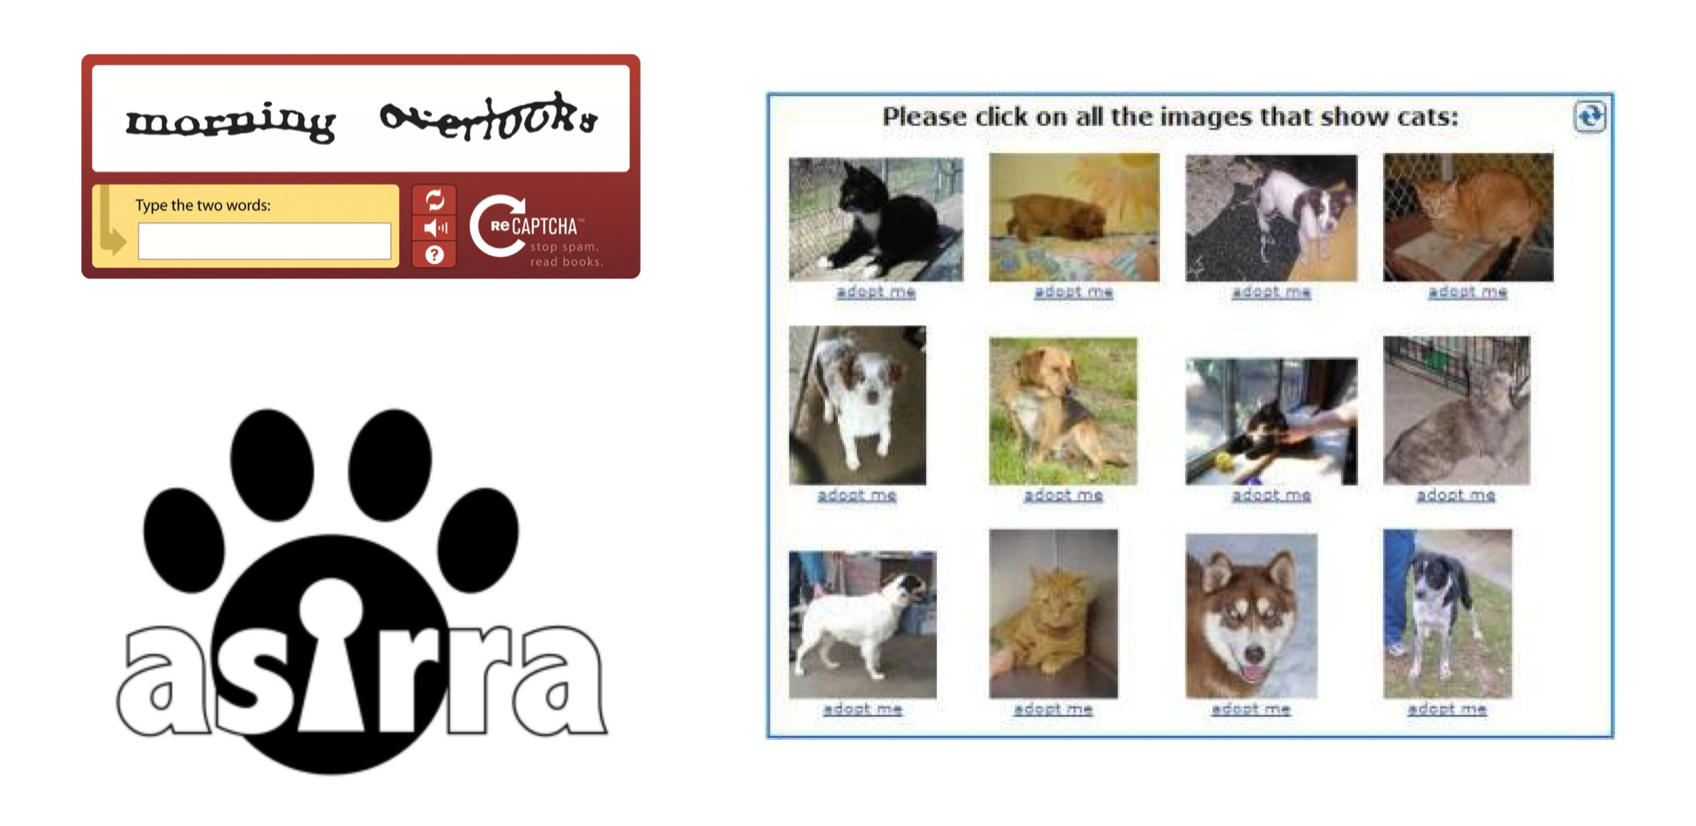
\includegraphics[width=.9\linewidth]{asira_capcha.png}
\end{center}
\end{frame}


\begin{frame}{Затравка (2006)}
\begin{wideitemize}
	\item Капча портит вид сайтов, довольно бесполезная, в Microsoft придумывают в 2006 году новый вид капчи. Надо отличать котов от собак. 
	\item В то время разделение собак от кошек было очень сложной задачей, лучшая точность была $0.6$. 
	\item У нас ест 12 картинок, робот нагнёт нас с вероятностью $0.6^{12}$. 
	\item Пул картинок пополнялся фотографиями из приютов. 
\end{wideitemize} 
\end{frame}


\begin{frame}{В 2014 проект закрыли}
\begin{center}
	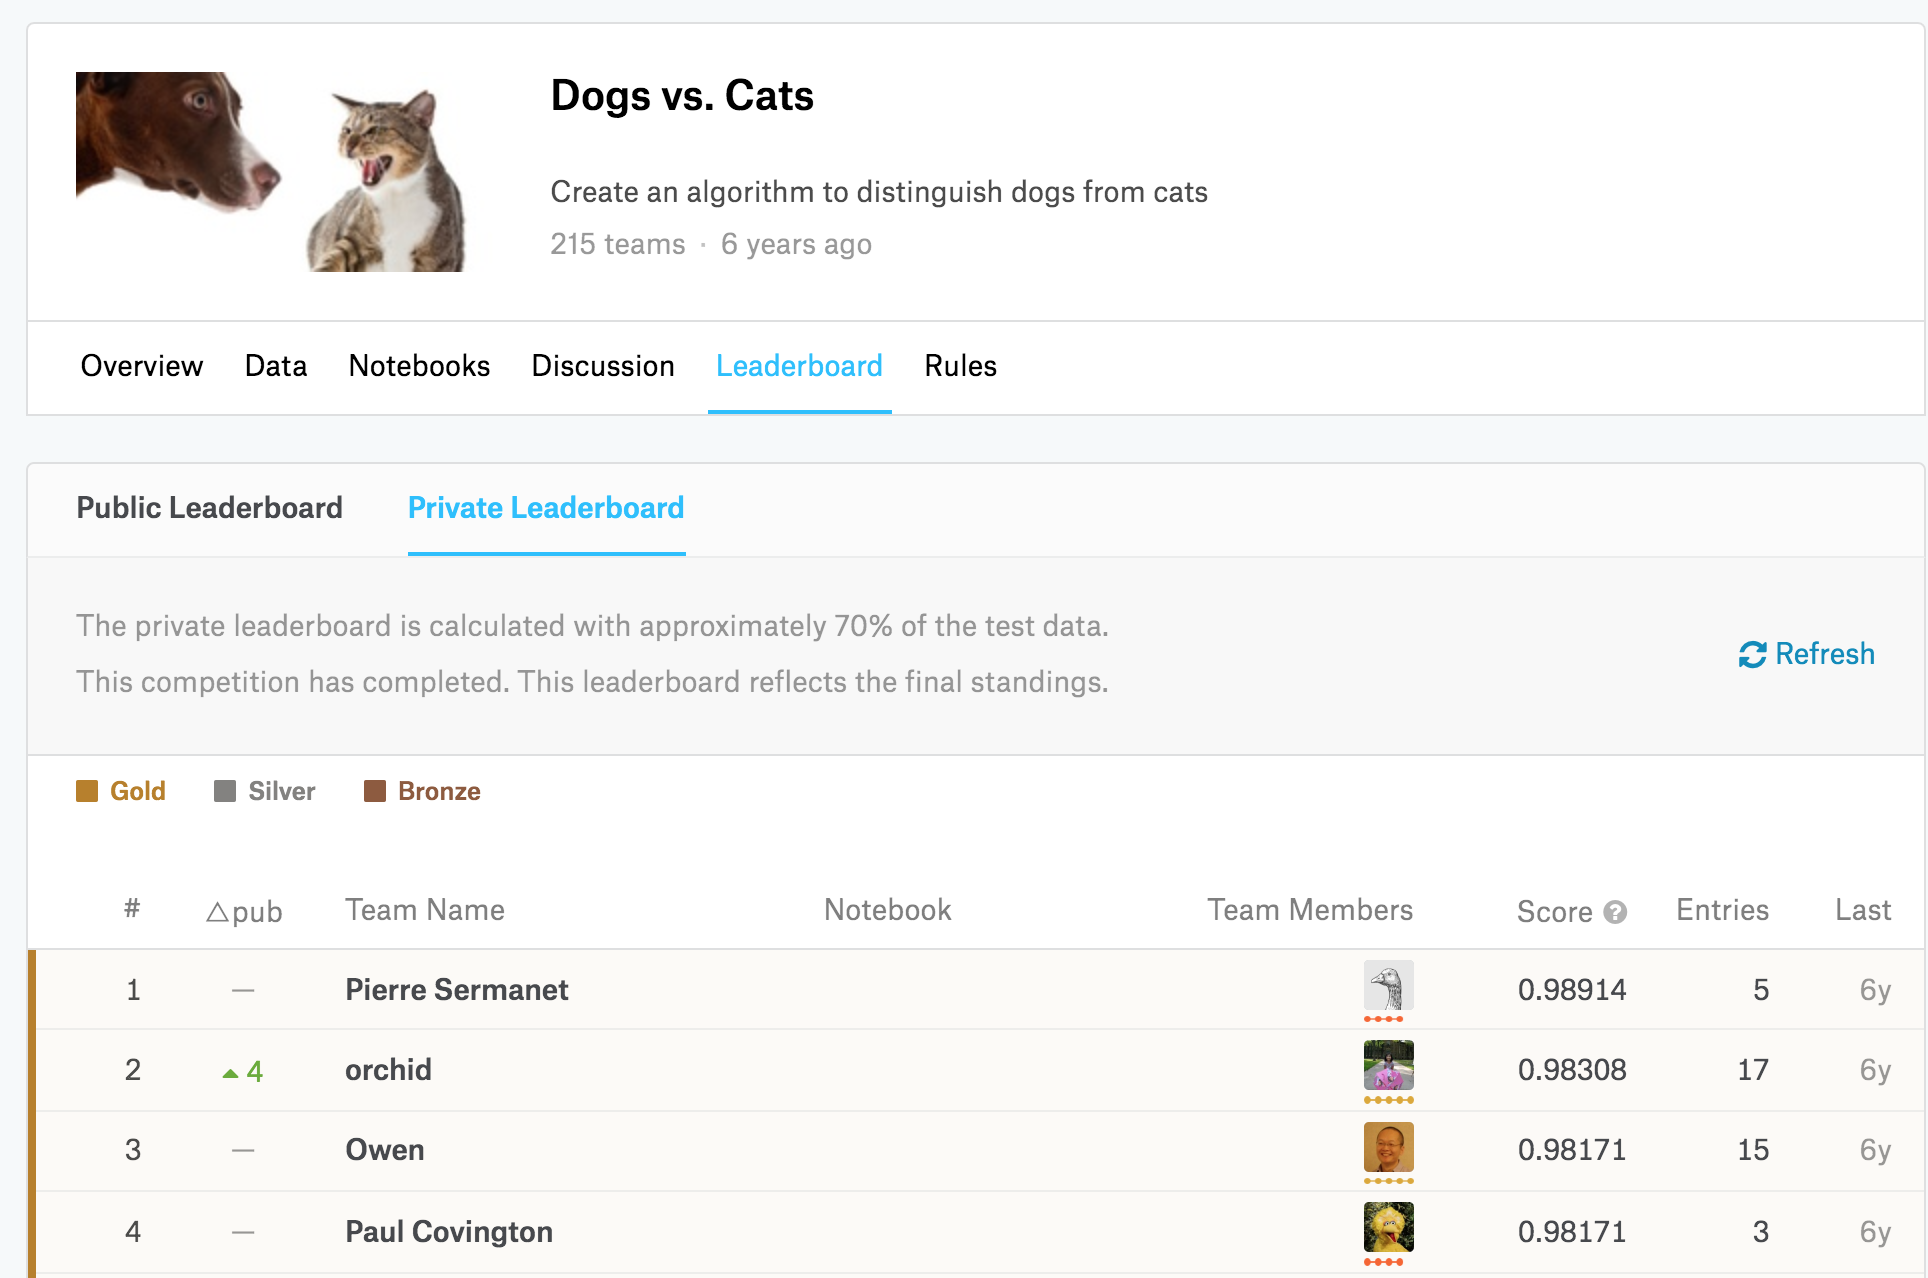
\includegraphics[width=.7\linewidth]{dogs_vs_cat.png}
\end{center}
\end{frame}


\begin{transitionframe}
	\begin{center}
		\Huge Как видит компьютер
	\end{center}
\end{transitionframe}


\begin{frame}{Картинка — тензор}
\begin{itemize}
	\item Каждая картинка — это матрица из пикселей
	
	\item Каждый пиксель обладает яркостью по шкале от $0$ до $255$ 
	
\end{itemize}
\begin{center}
	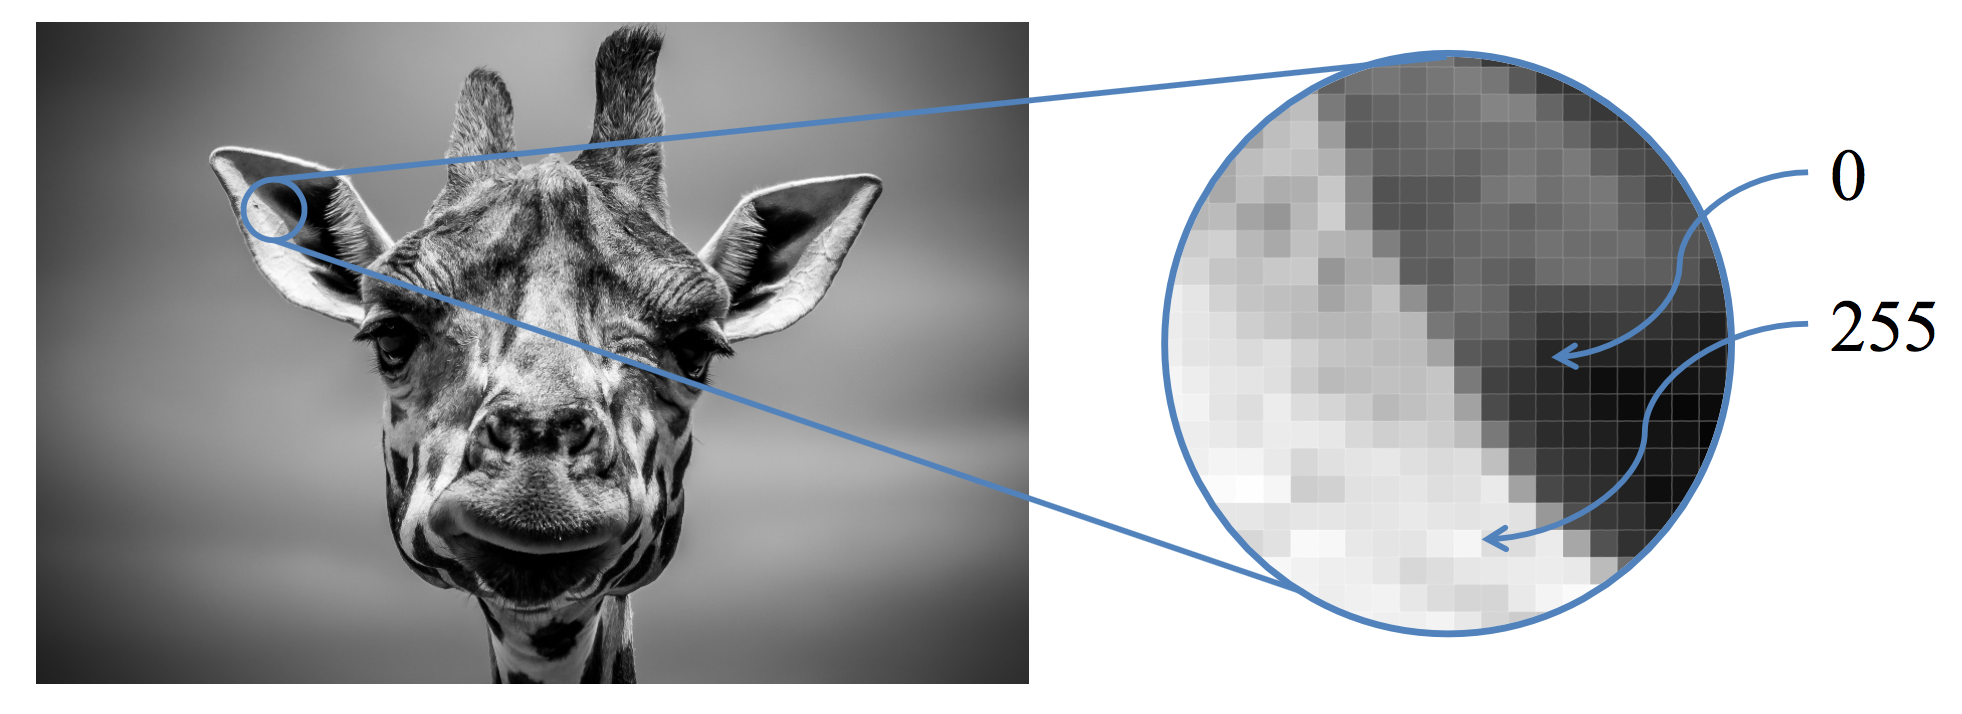
\includegraphics[width=.7\linewidth]{pixels.png}
\end{center}
\end{frame}

\begin{frame}{Картинка — тензор}
\begin{itemize}
	\item Цветное изображение имеет три канала пикселей: красный, зелёный и синий (rgb), размерность изображения $5 \times 5 \times 3$
\end{itemize}

\begin{center}
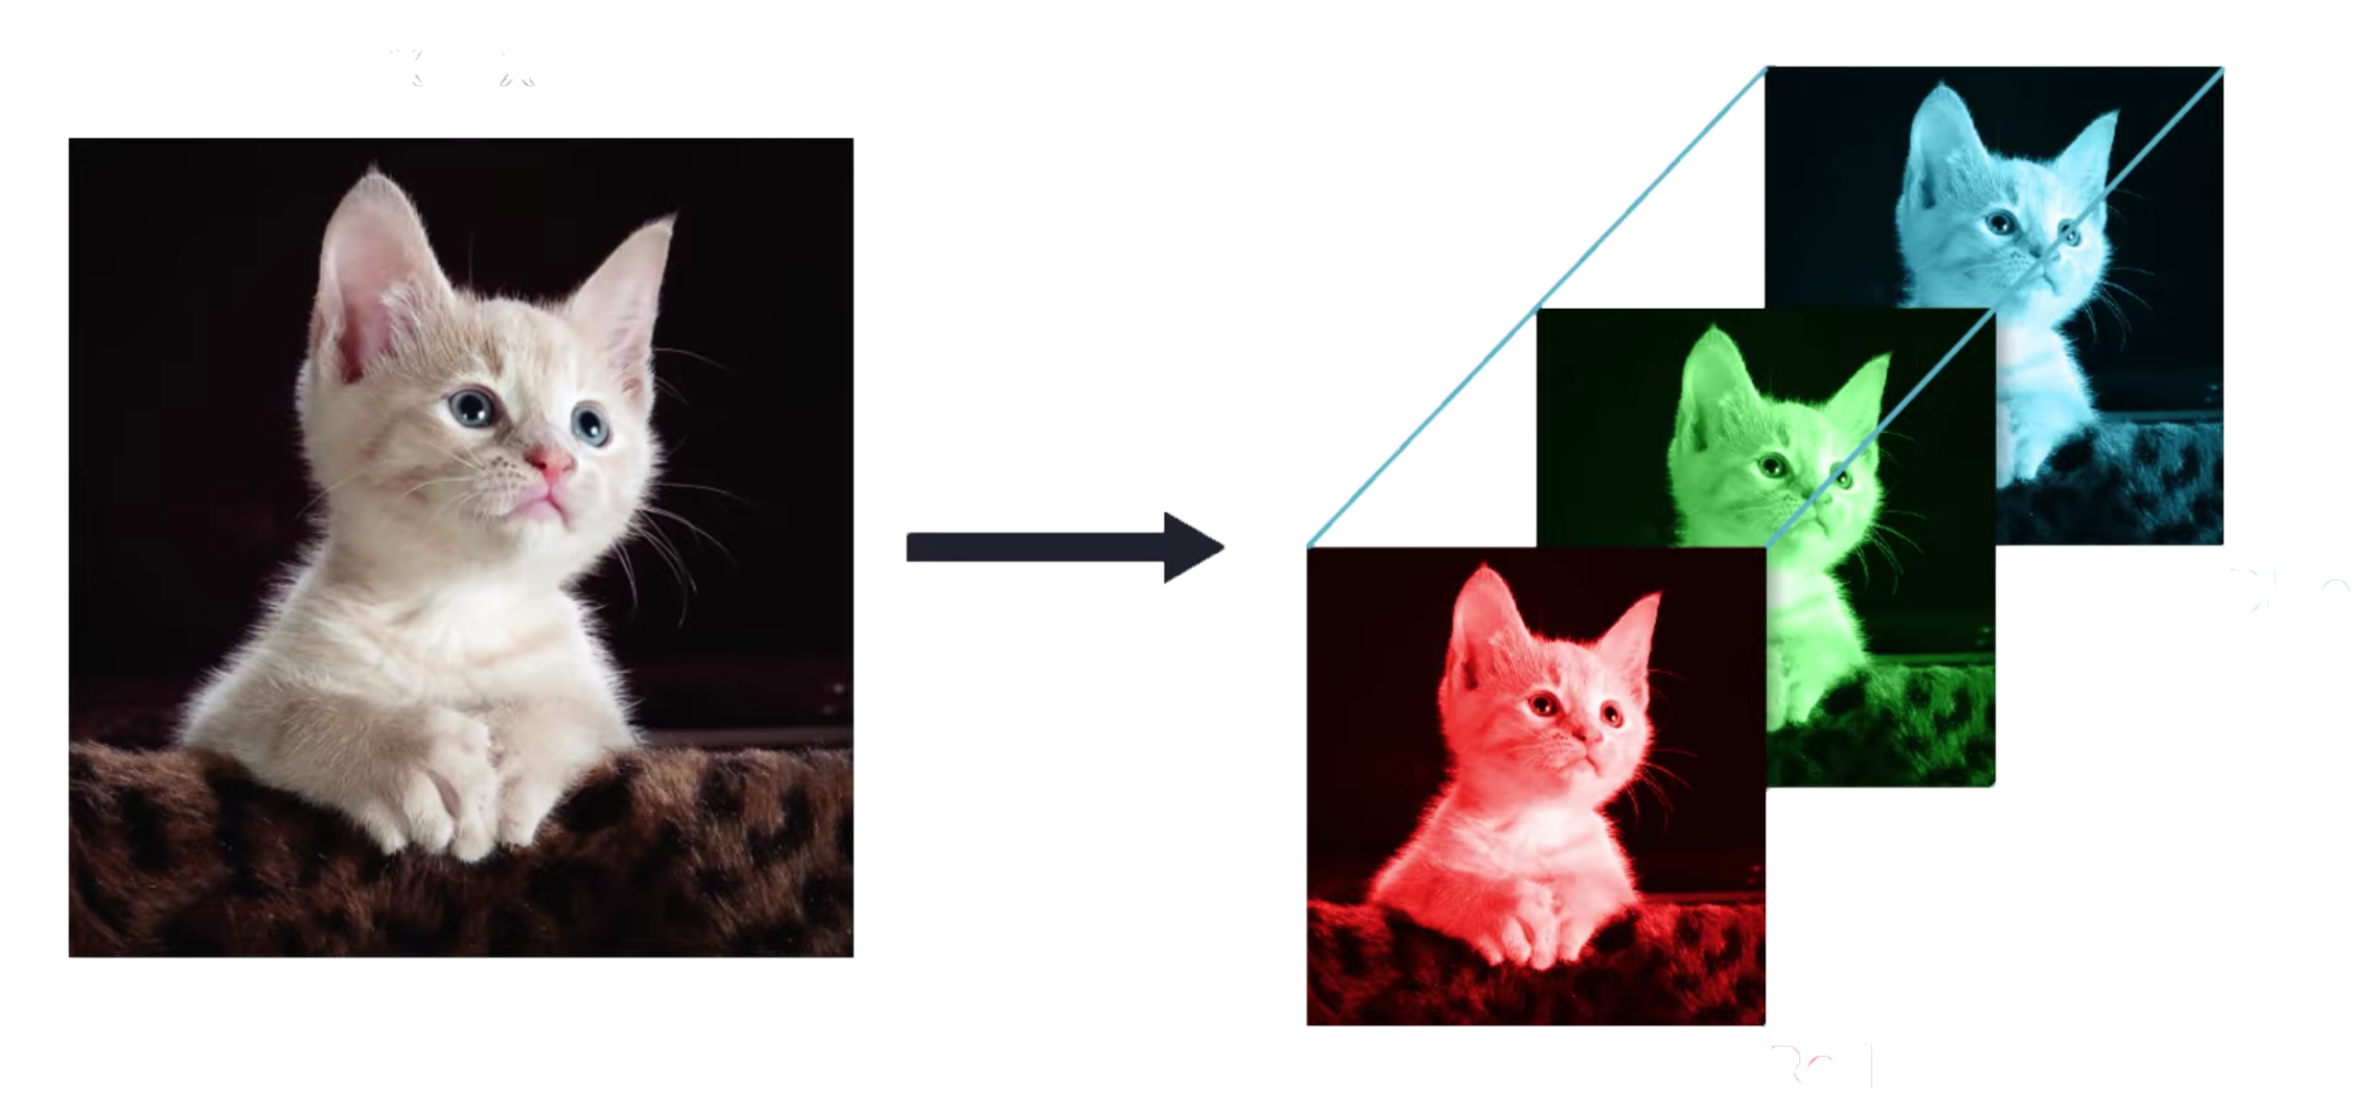
\includegraphics[width=.7\linewidth]{pixels2_clean.png}
\end{center}
\end{frame}

\begin{frame}{Картинка — тензор}
\begin{center}
	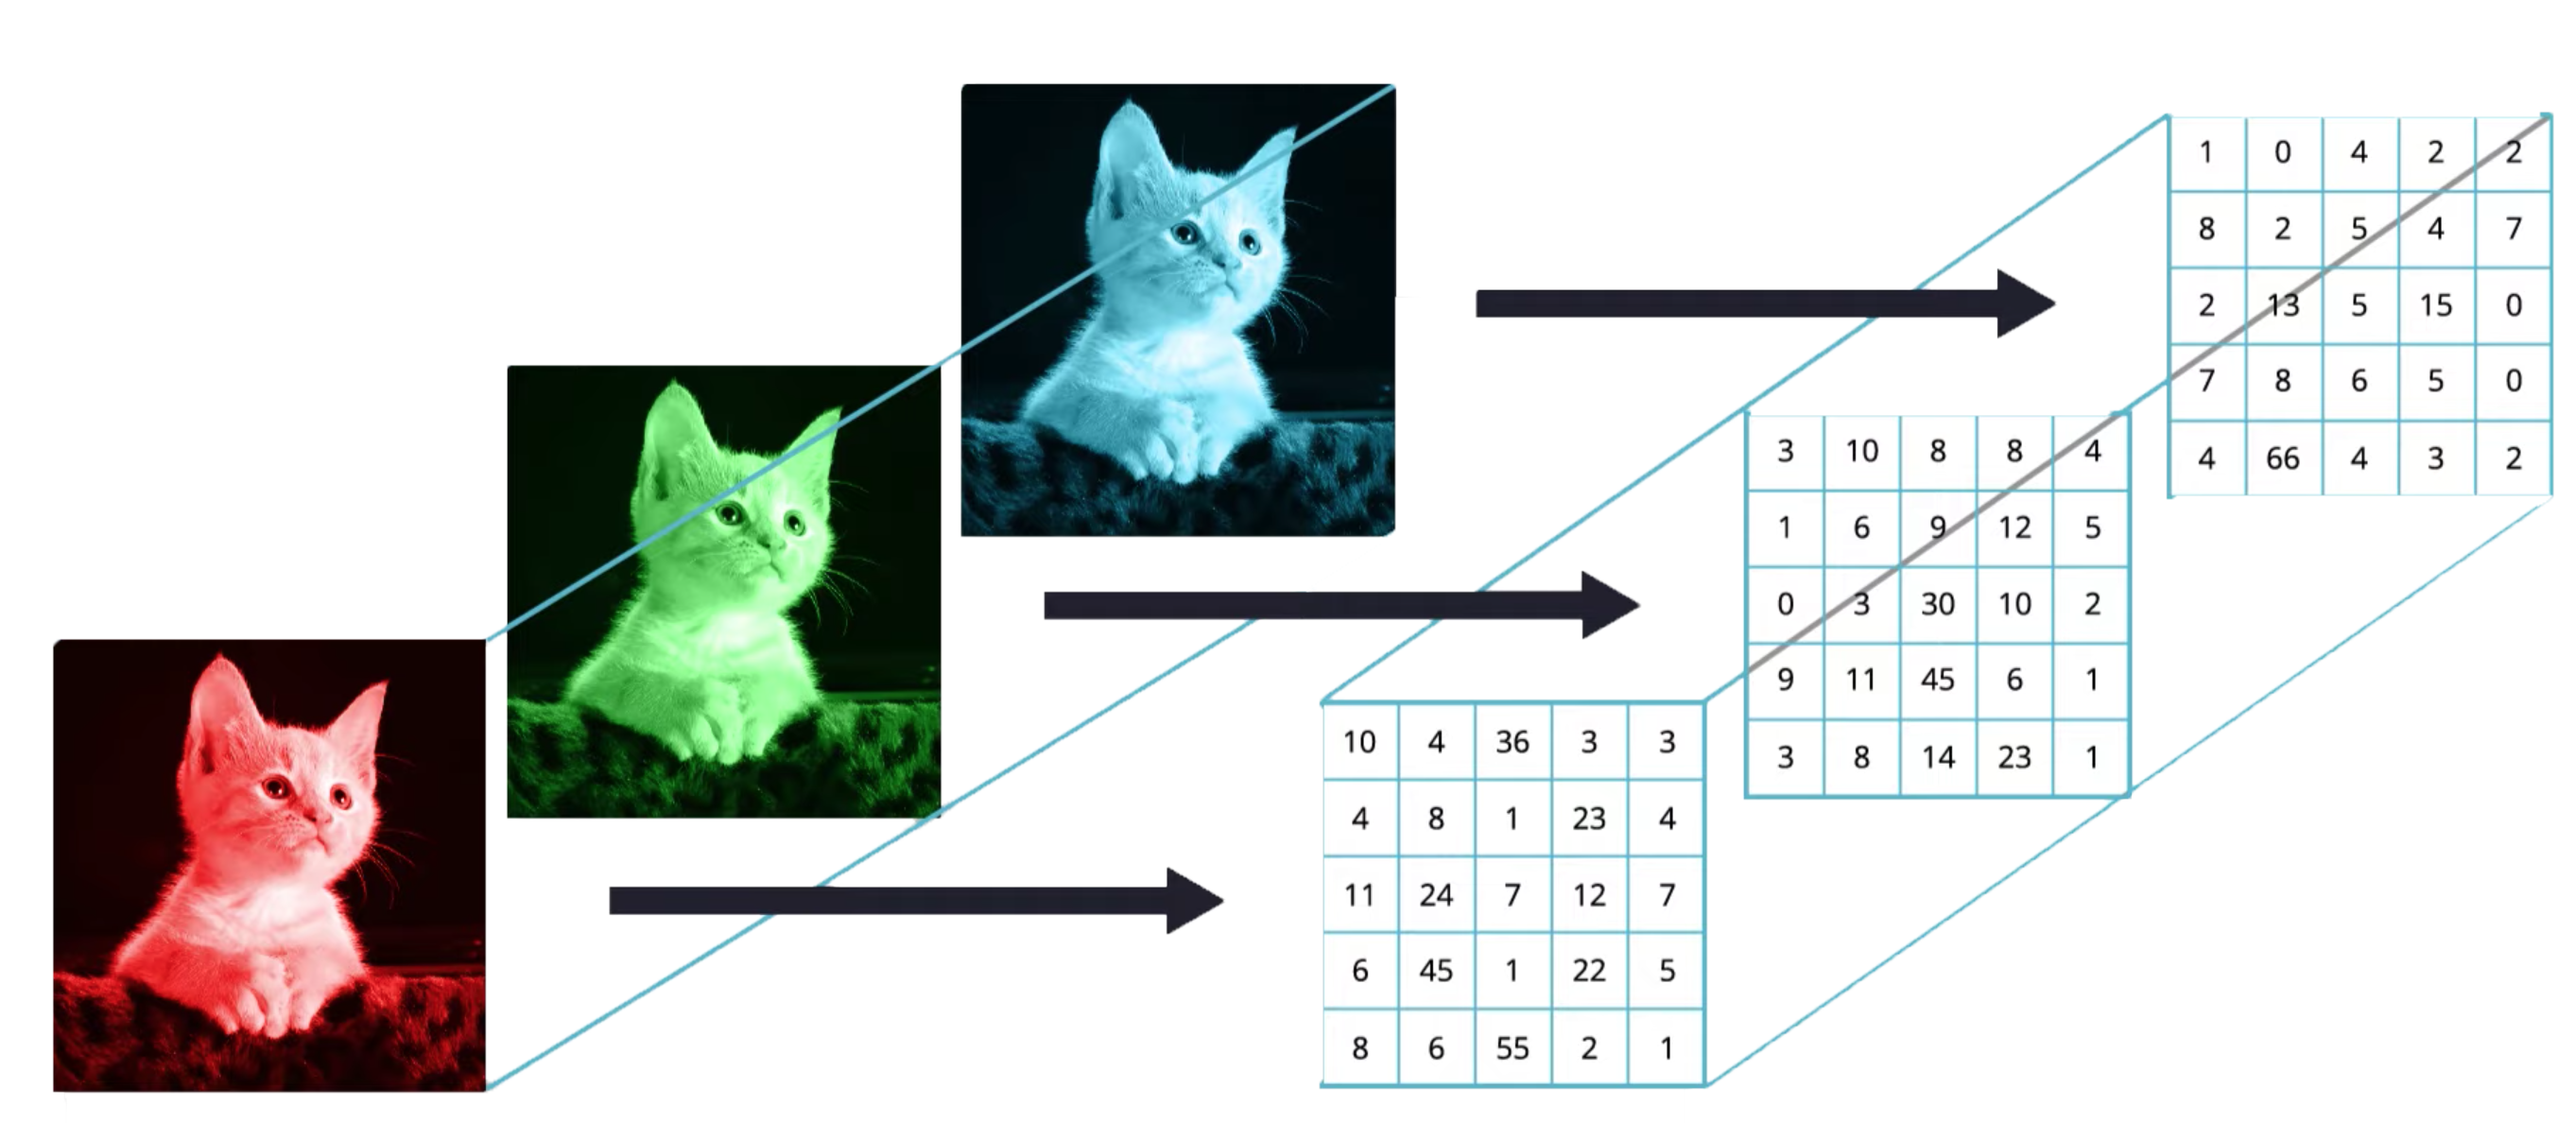
\includegraphics[width=.8\linewidth]{pixels3_clean.png}
\end{center}
\end{frame}


\begin{frame}{Картинка — тензор}
\begin{center}
	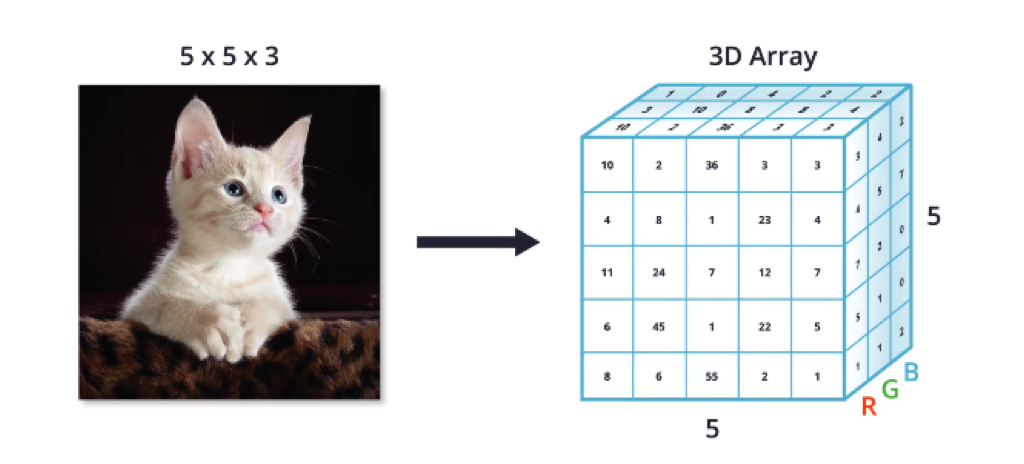
\includegraphics[width=.8\linewidth]{cat_cube.png}
\end{center}
\end{frame}




% сделать на следущей итерации курса более подробные слайды про тензоры 


\begin{frame}{Обычная сетка}
\begin{center}
	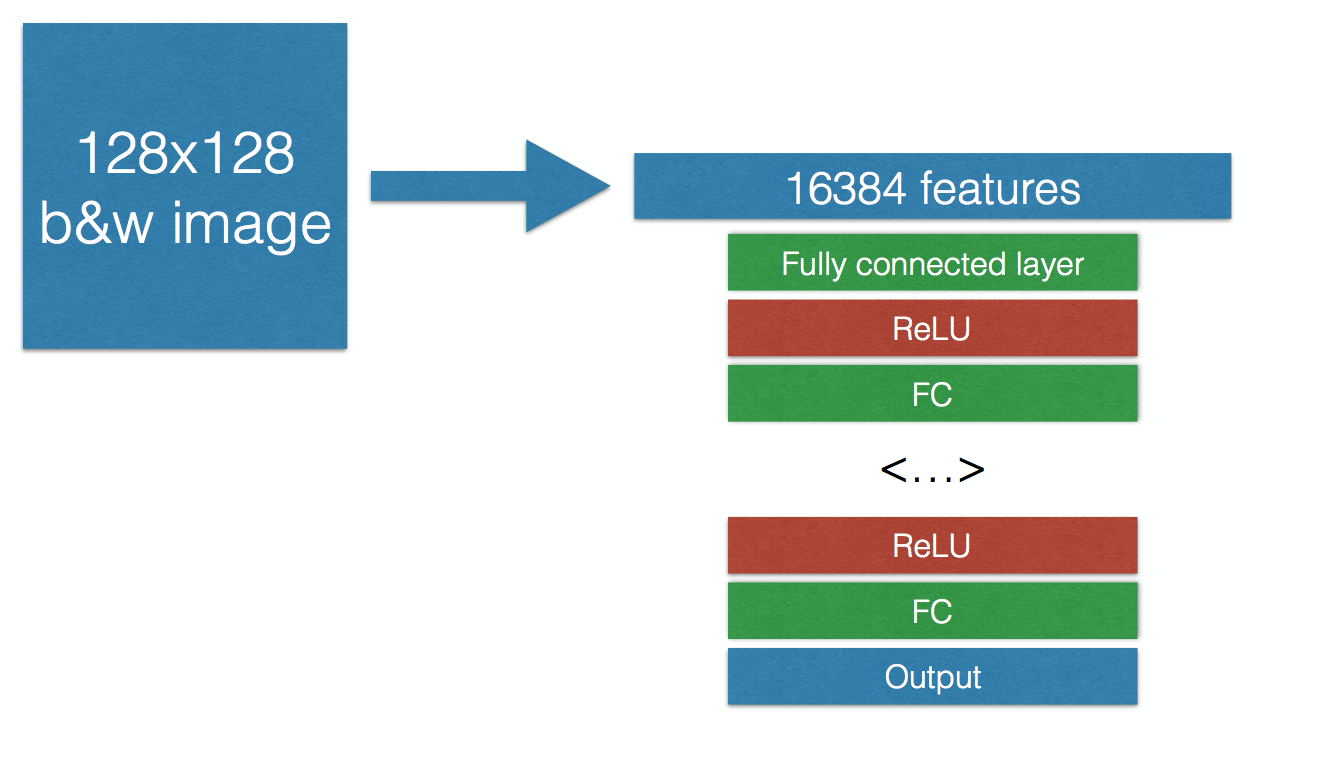
\includegraphics[width=.55\linewidth]{not_conv.png}
\end{center}

\begin{wideitemize}
	\item Очень много весов 
	\item Теряется информация о взаимном расположении пикселей
	\item Изображение в разных местах картинки даёт разные веса
\end{wideitemize}
\end{frame}


\begin{frame}
\begin{center}
	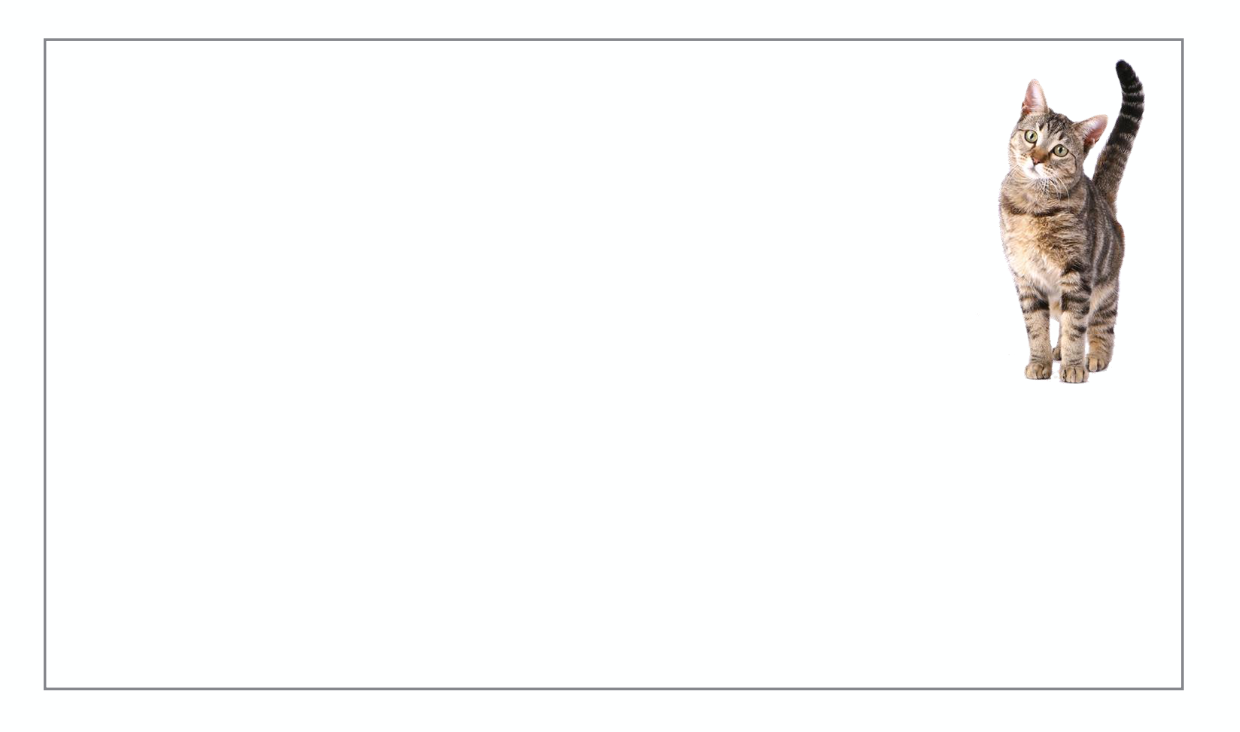
\includegraphics[width=.8\linewidth]{cat_1.png}
\end{center}
\end{frame}


\begin{frame}
\begin{center}
	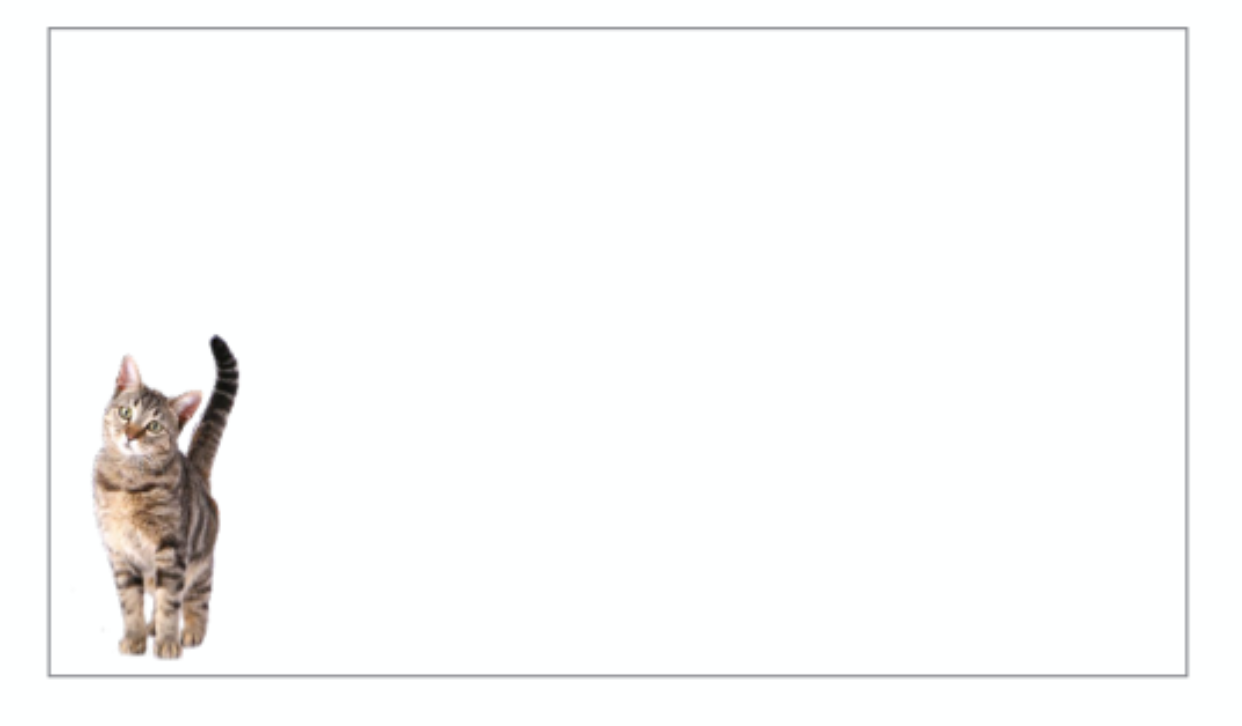
\includegraphics[width=.8\linewidth]{cat_2.png}
\end{center}
\end{frame}


\begin{frame}
\begin{center}
	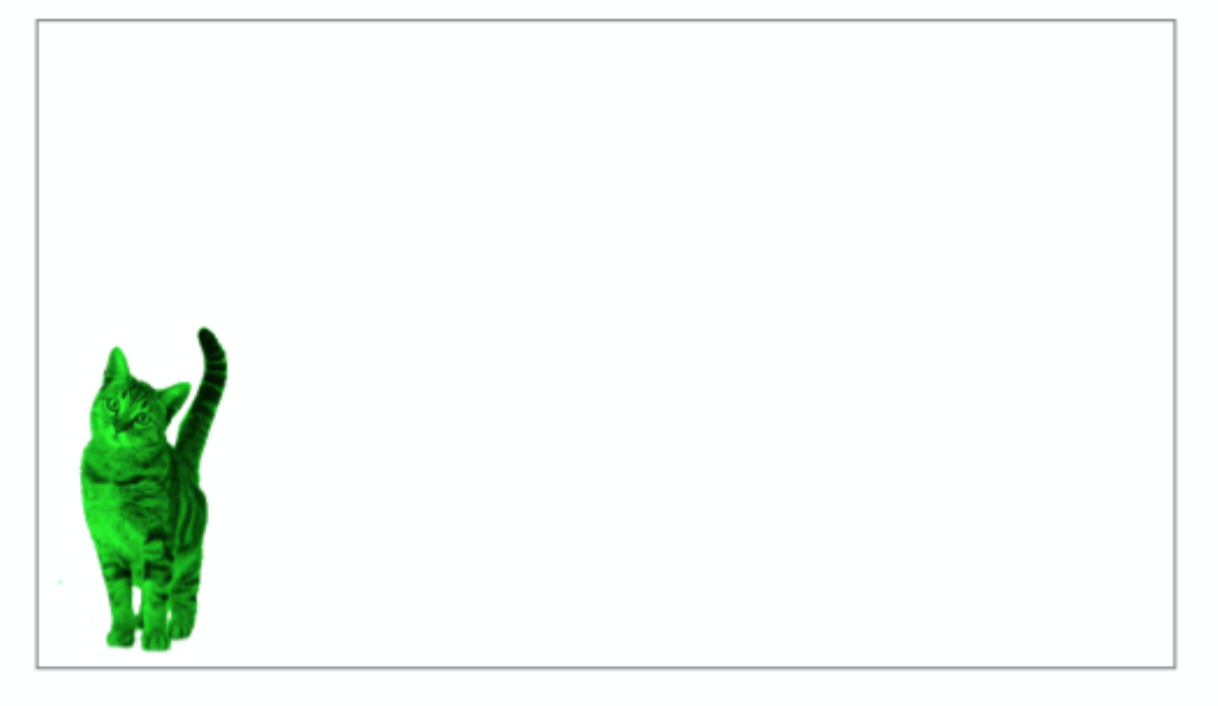
\includegraphics[width=.8\linewidth]{cat_3.png}
\end{center}
\end{frame}


\begin{frame}{Обычная сетка}
\begin{wideitemize}
	\item Хотим, чтобы информация не терялась
	\item Хотим одинаковые веса $\Rightarrow$ {\color{red} свёртка} 
\end{wideitemize}
\end{frame}


\begin{transitionframe}
	\begin{center}
		\Huge Свёртка
	\end{center}
\end{transitionframe}


{
	\usebackgroundtemplate{ 
		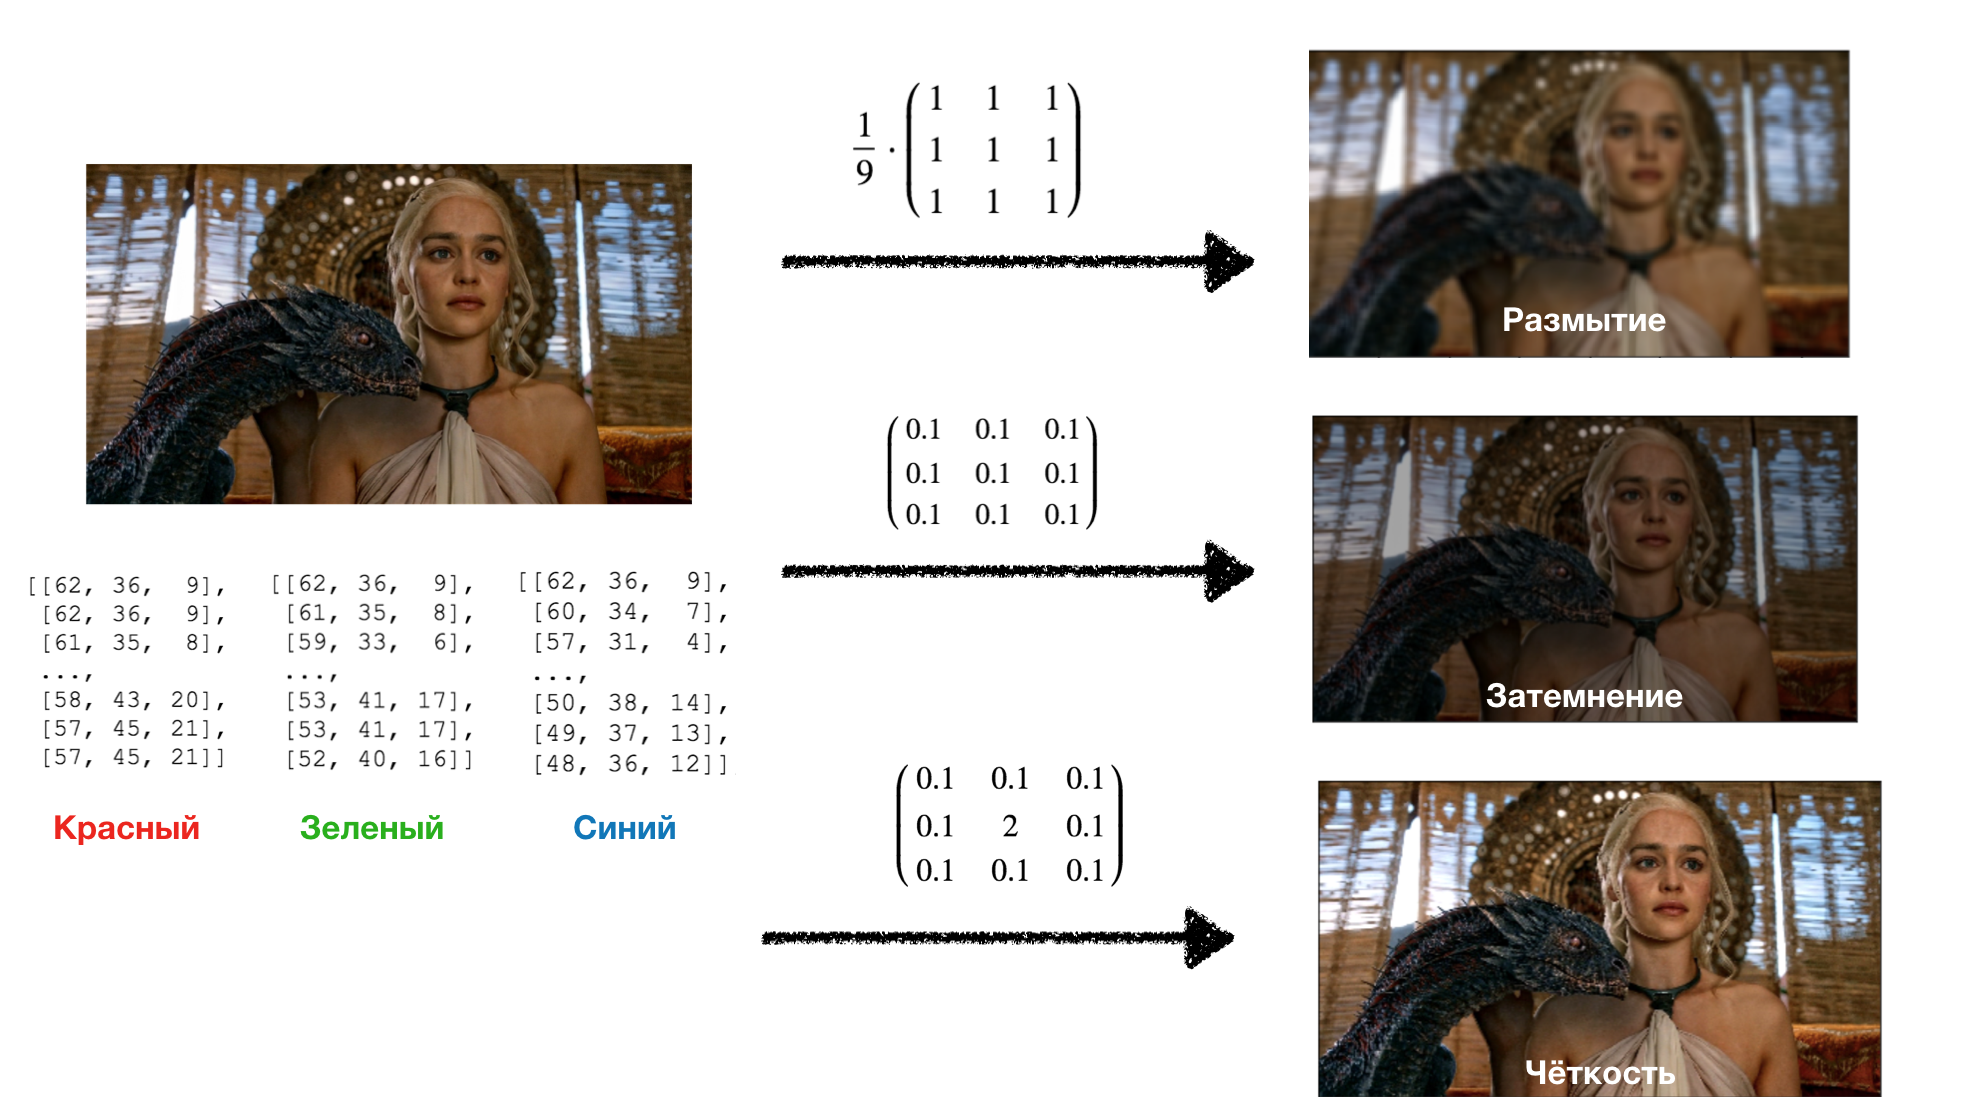
\includegraphics[width=\paperwidth]{emilia.png}}
	\begin{frame}
\end{frame}
}


\begin{frame}{Свёртка}
\begin{wideitemize}
	\item Разные ядра помогают накладывать на кртинку различные эффекты
	\item Какие-то ядра помогают искать границы
	\item \alert{Идея:} возможно, с помощью некоторых ядер можно искать что-то кроме границ...
\end{wideitemize}
\end{frame}



\begin{frame}{Классификатор слэшей}
\begin{center}
	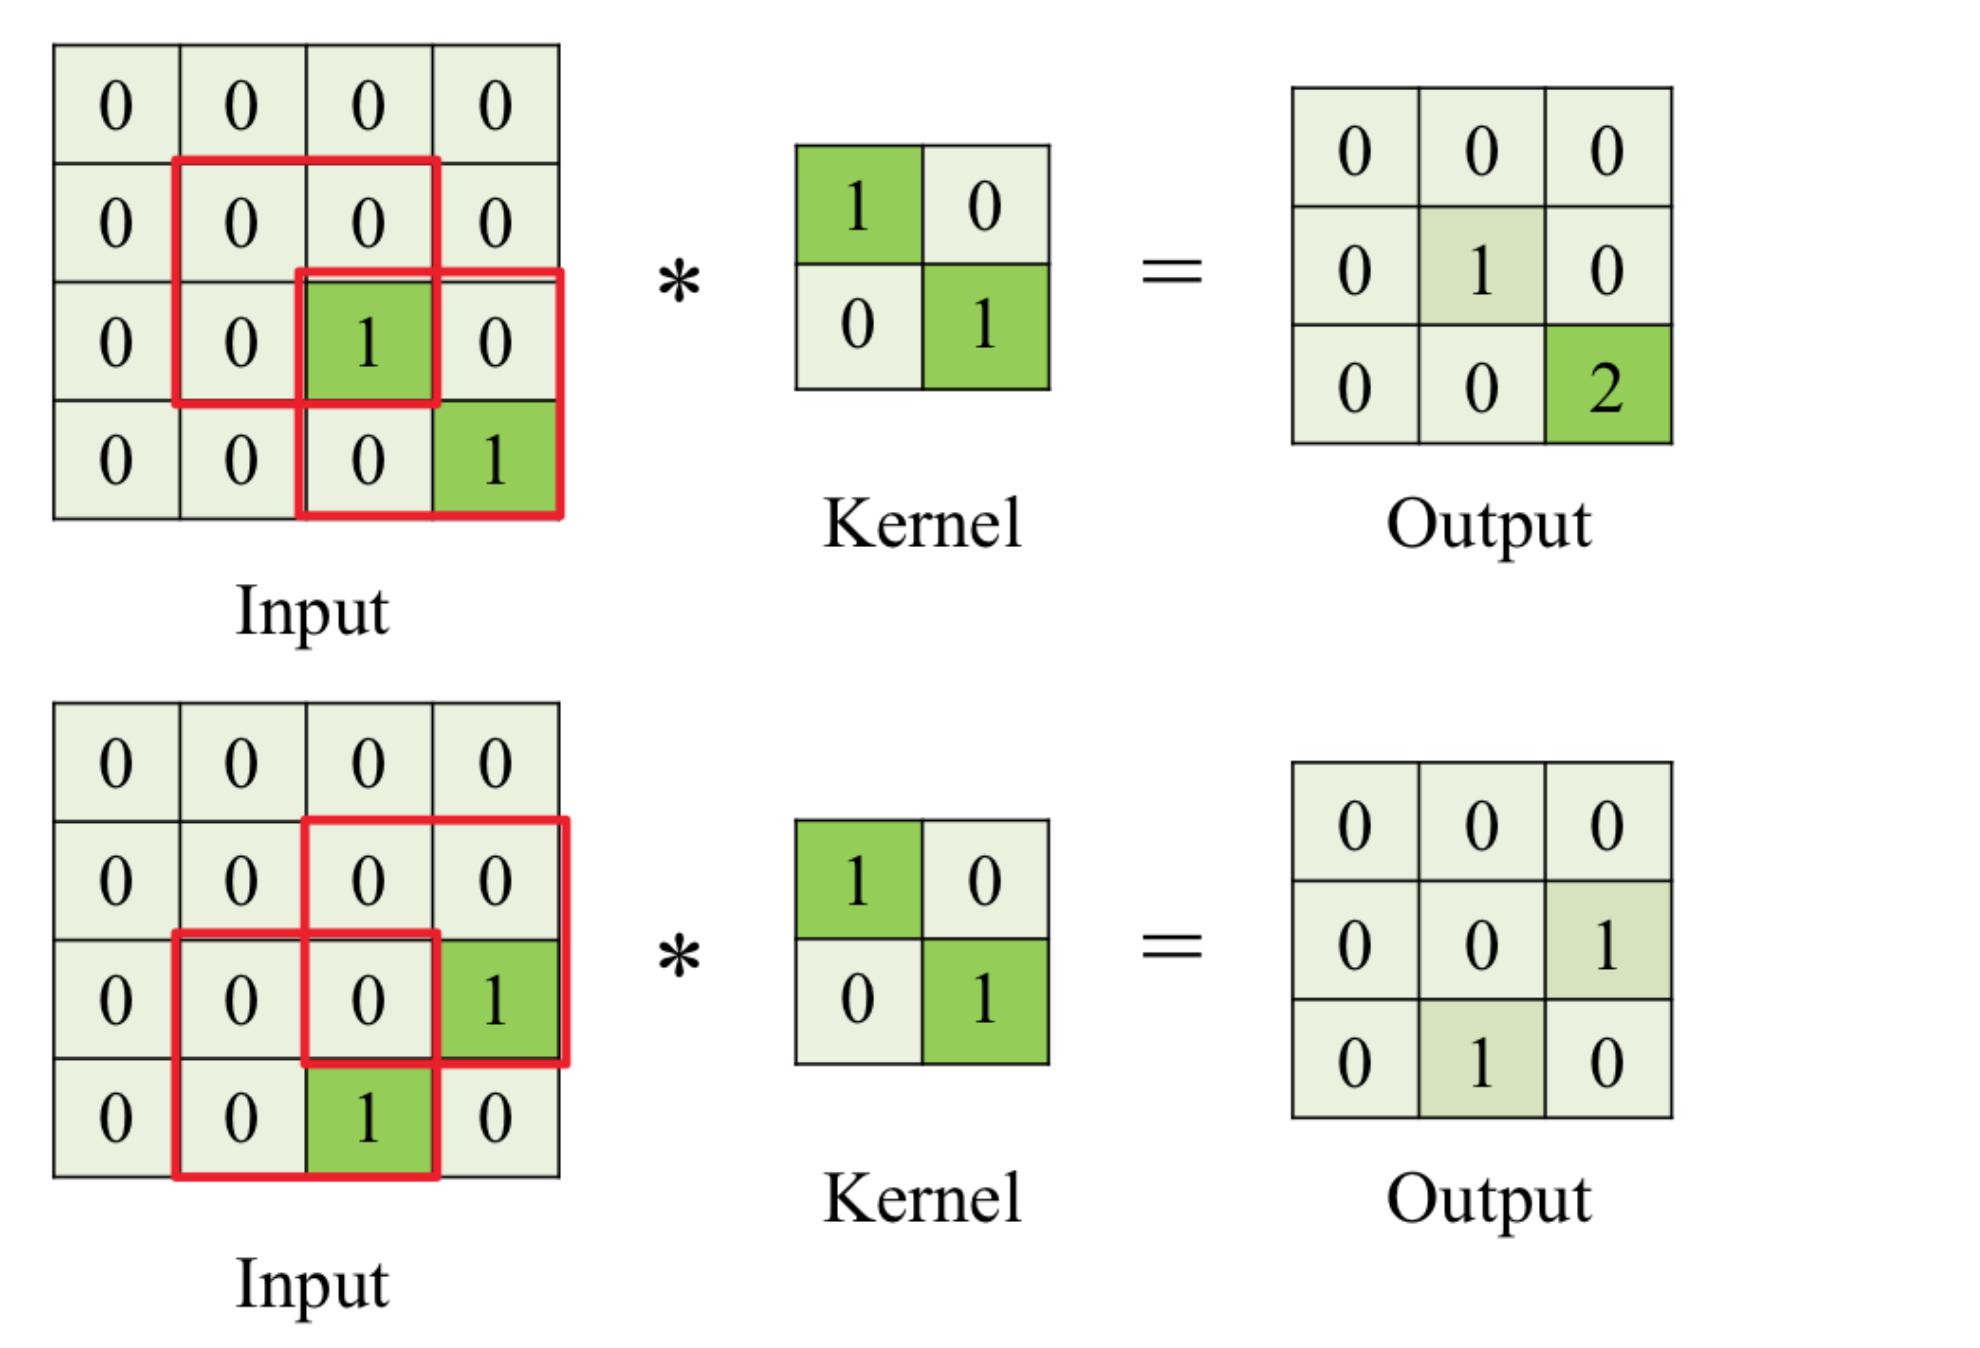
\includegraphics[width=.75\linewidth]{conv_1.png}
\end{center}
\end{frame}


\begin{frame}{Классификатор слэшей}
\begin{center}
	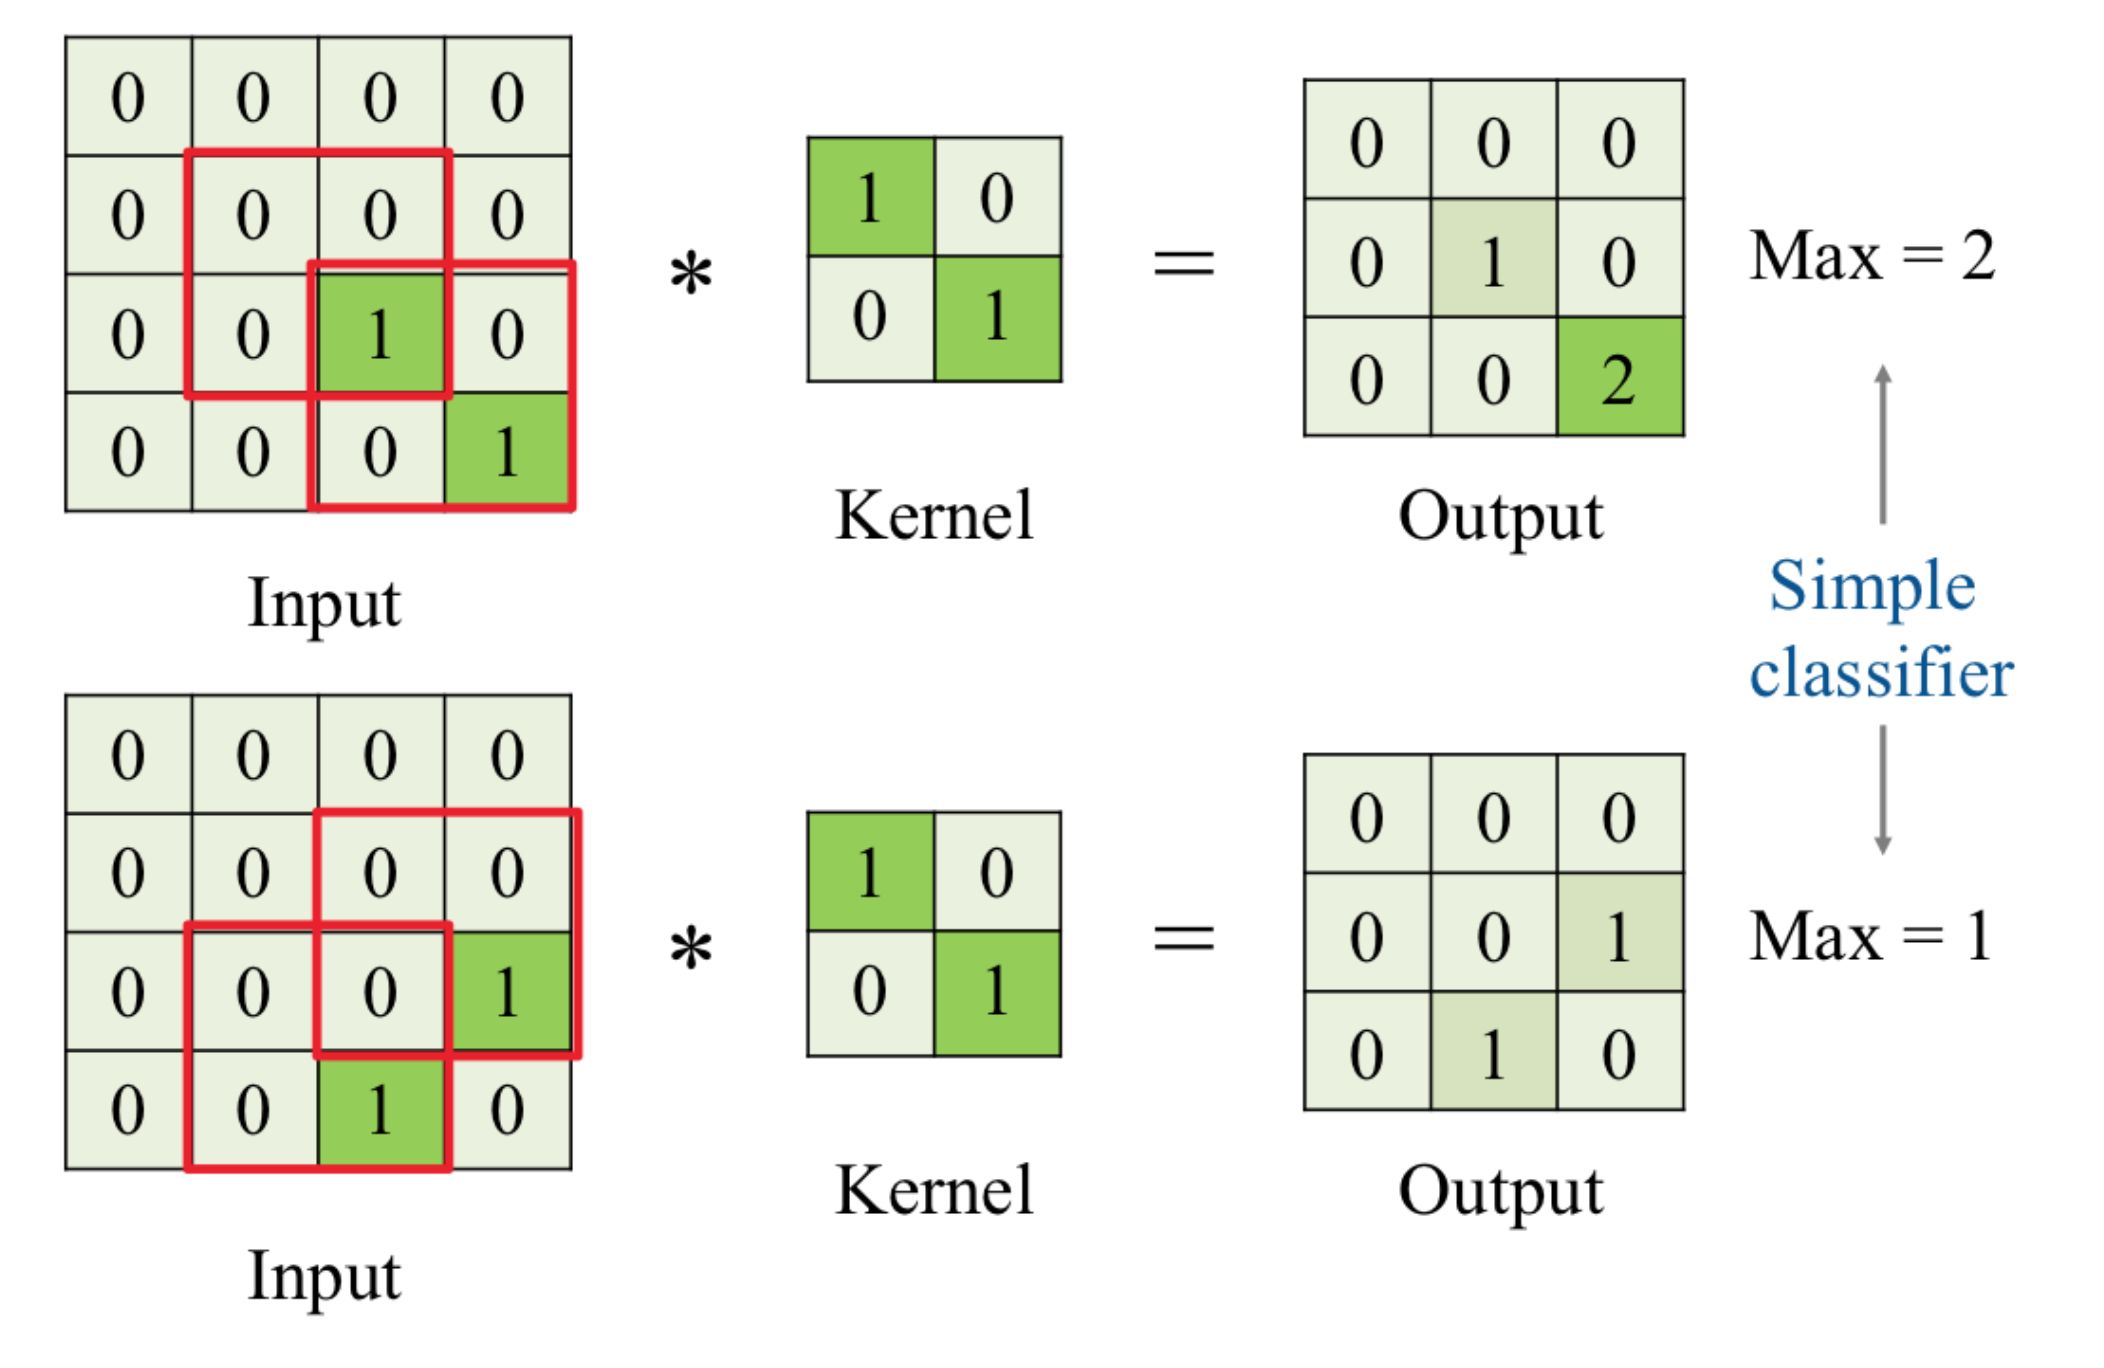
\includegraphics[width=.8\linewidth]{conv_2.png}
\end{center}
\end{frame}


\begin{frame}{Свёртка инвариантна к расположению}
\begin{center}
	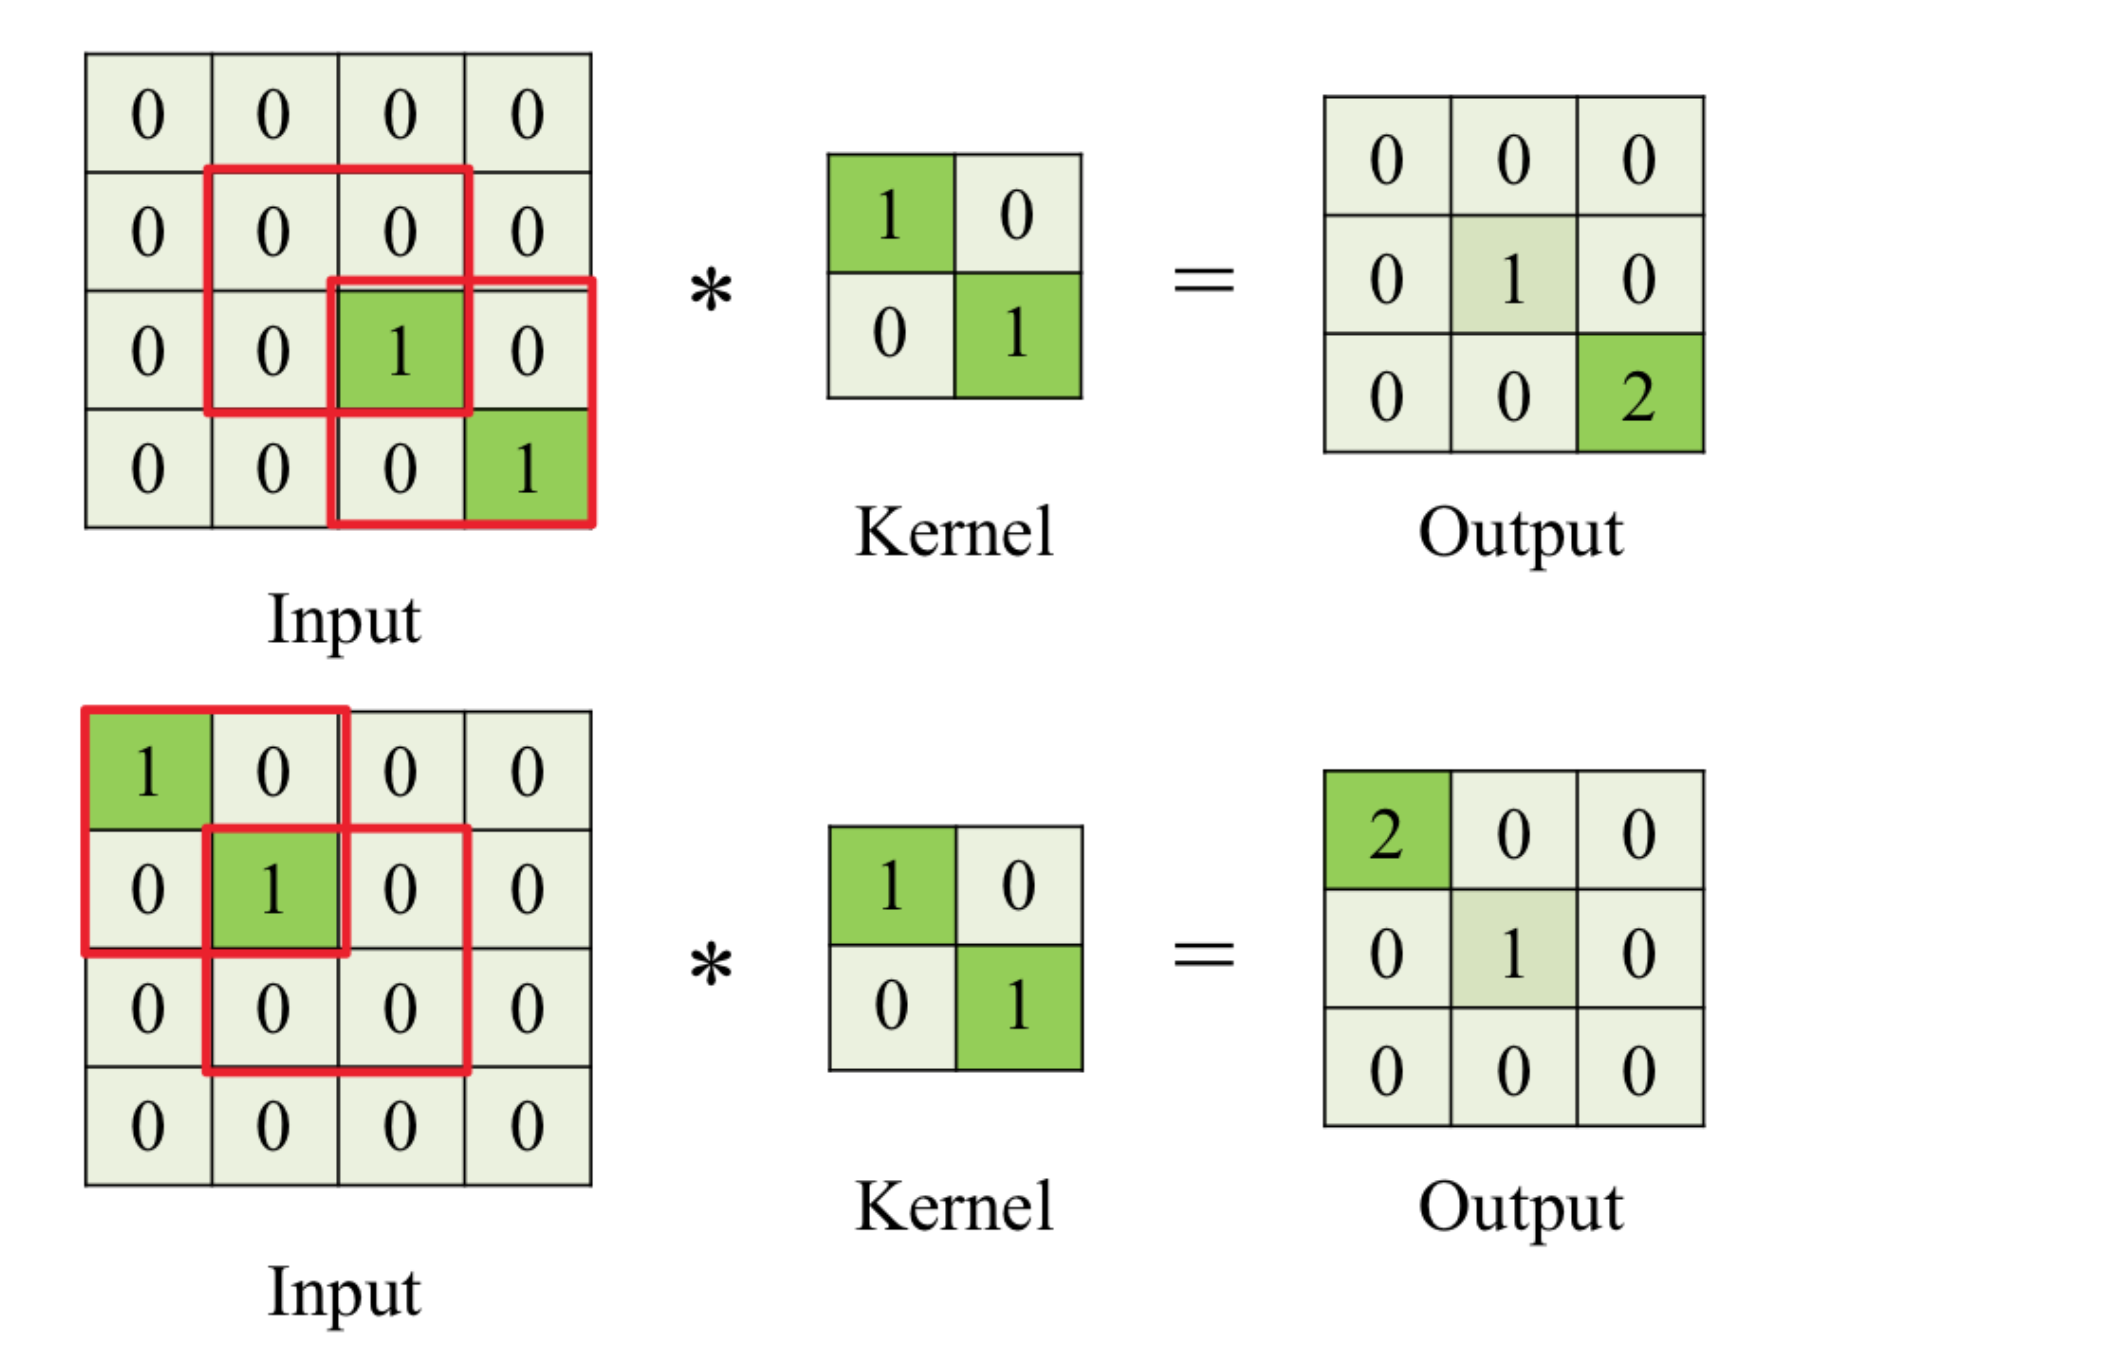
\includegraphics[width=.8\linewidth]{conv_3.png}
\end{center}
\end{frame}


\begin{frame}{Свёртка инвариантна к расположению}
\begin{center}
	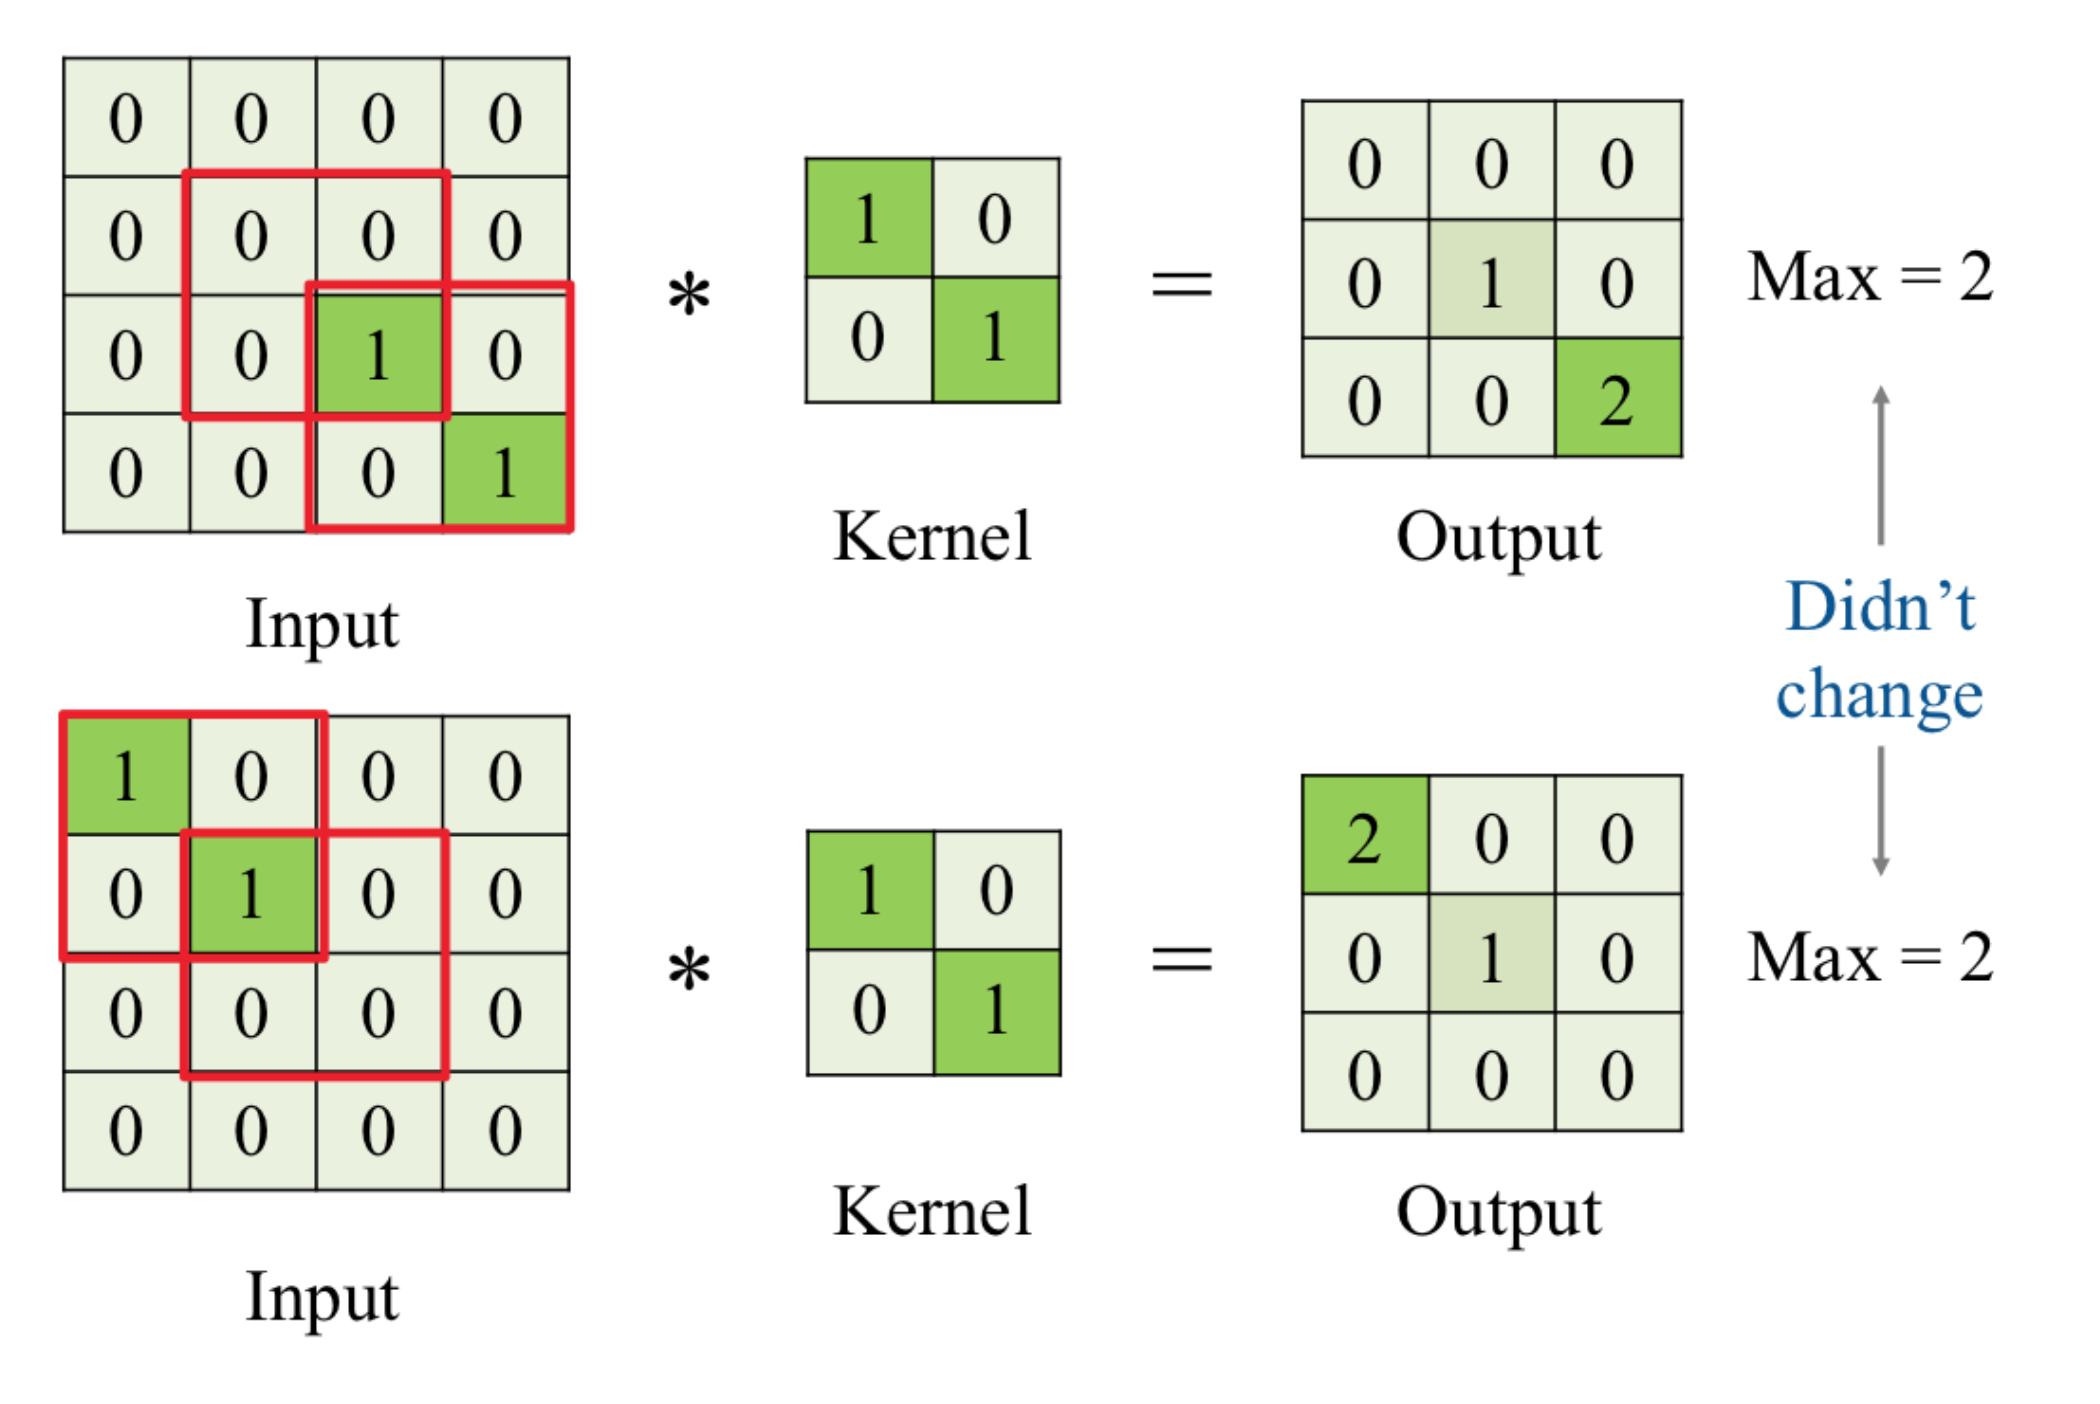
\includegraphics[width=.8\linewidth]{conv_4.png}
\end{center}
\end{frame}


\begin{frame}{Дополнение (Padding)}
\begin{center}
	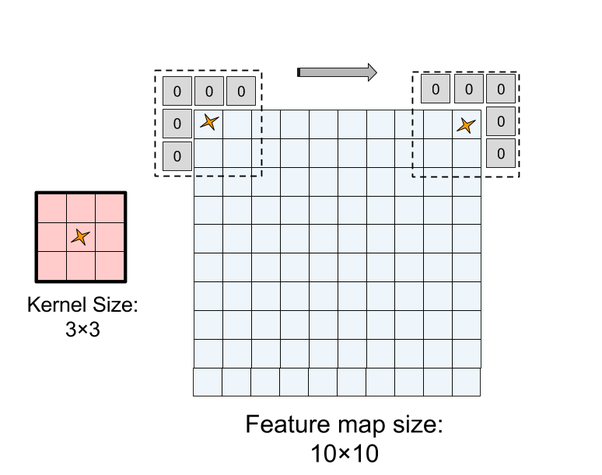
\includegraphics[width=.5\linewidth]{padding_1.png}
\end{center}
\vfill
\alert{Padding} используют, чтобы пространственная размерность картинки не уменьшалась после применения свёртки, это помогает не терять информацию на краях и избежать проблем с размерностями
\end{frame}


\begin{frame}{Дополнение (Padding)}
\begin{center}
	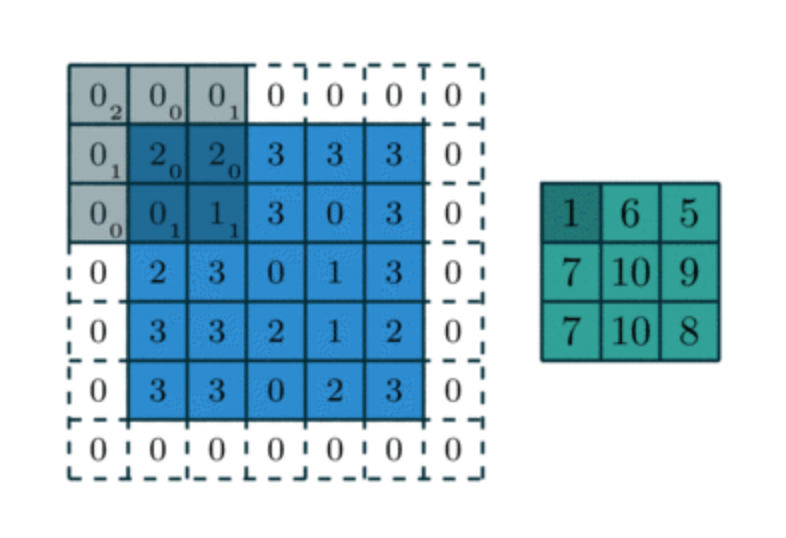
\includegraphics[width=.5\linewidth]{padding.png}
\end{center}
\end{frame}


\begin{frame}{Свёрточный слой}
\begin{center}
	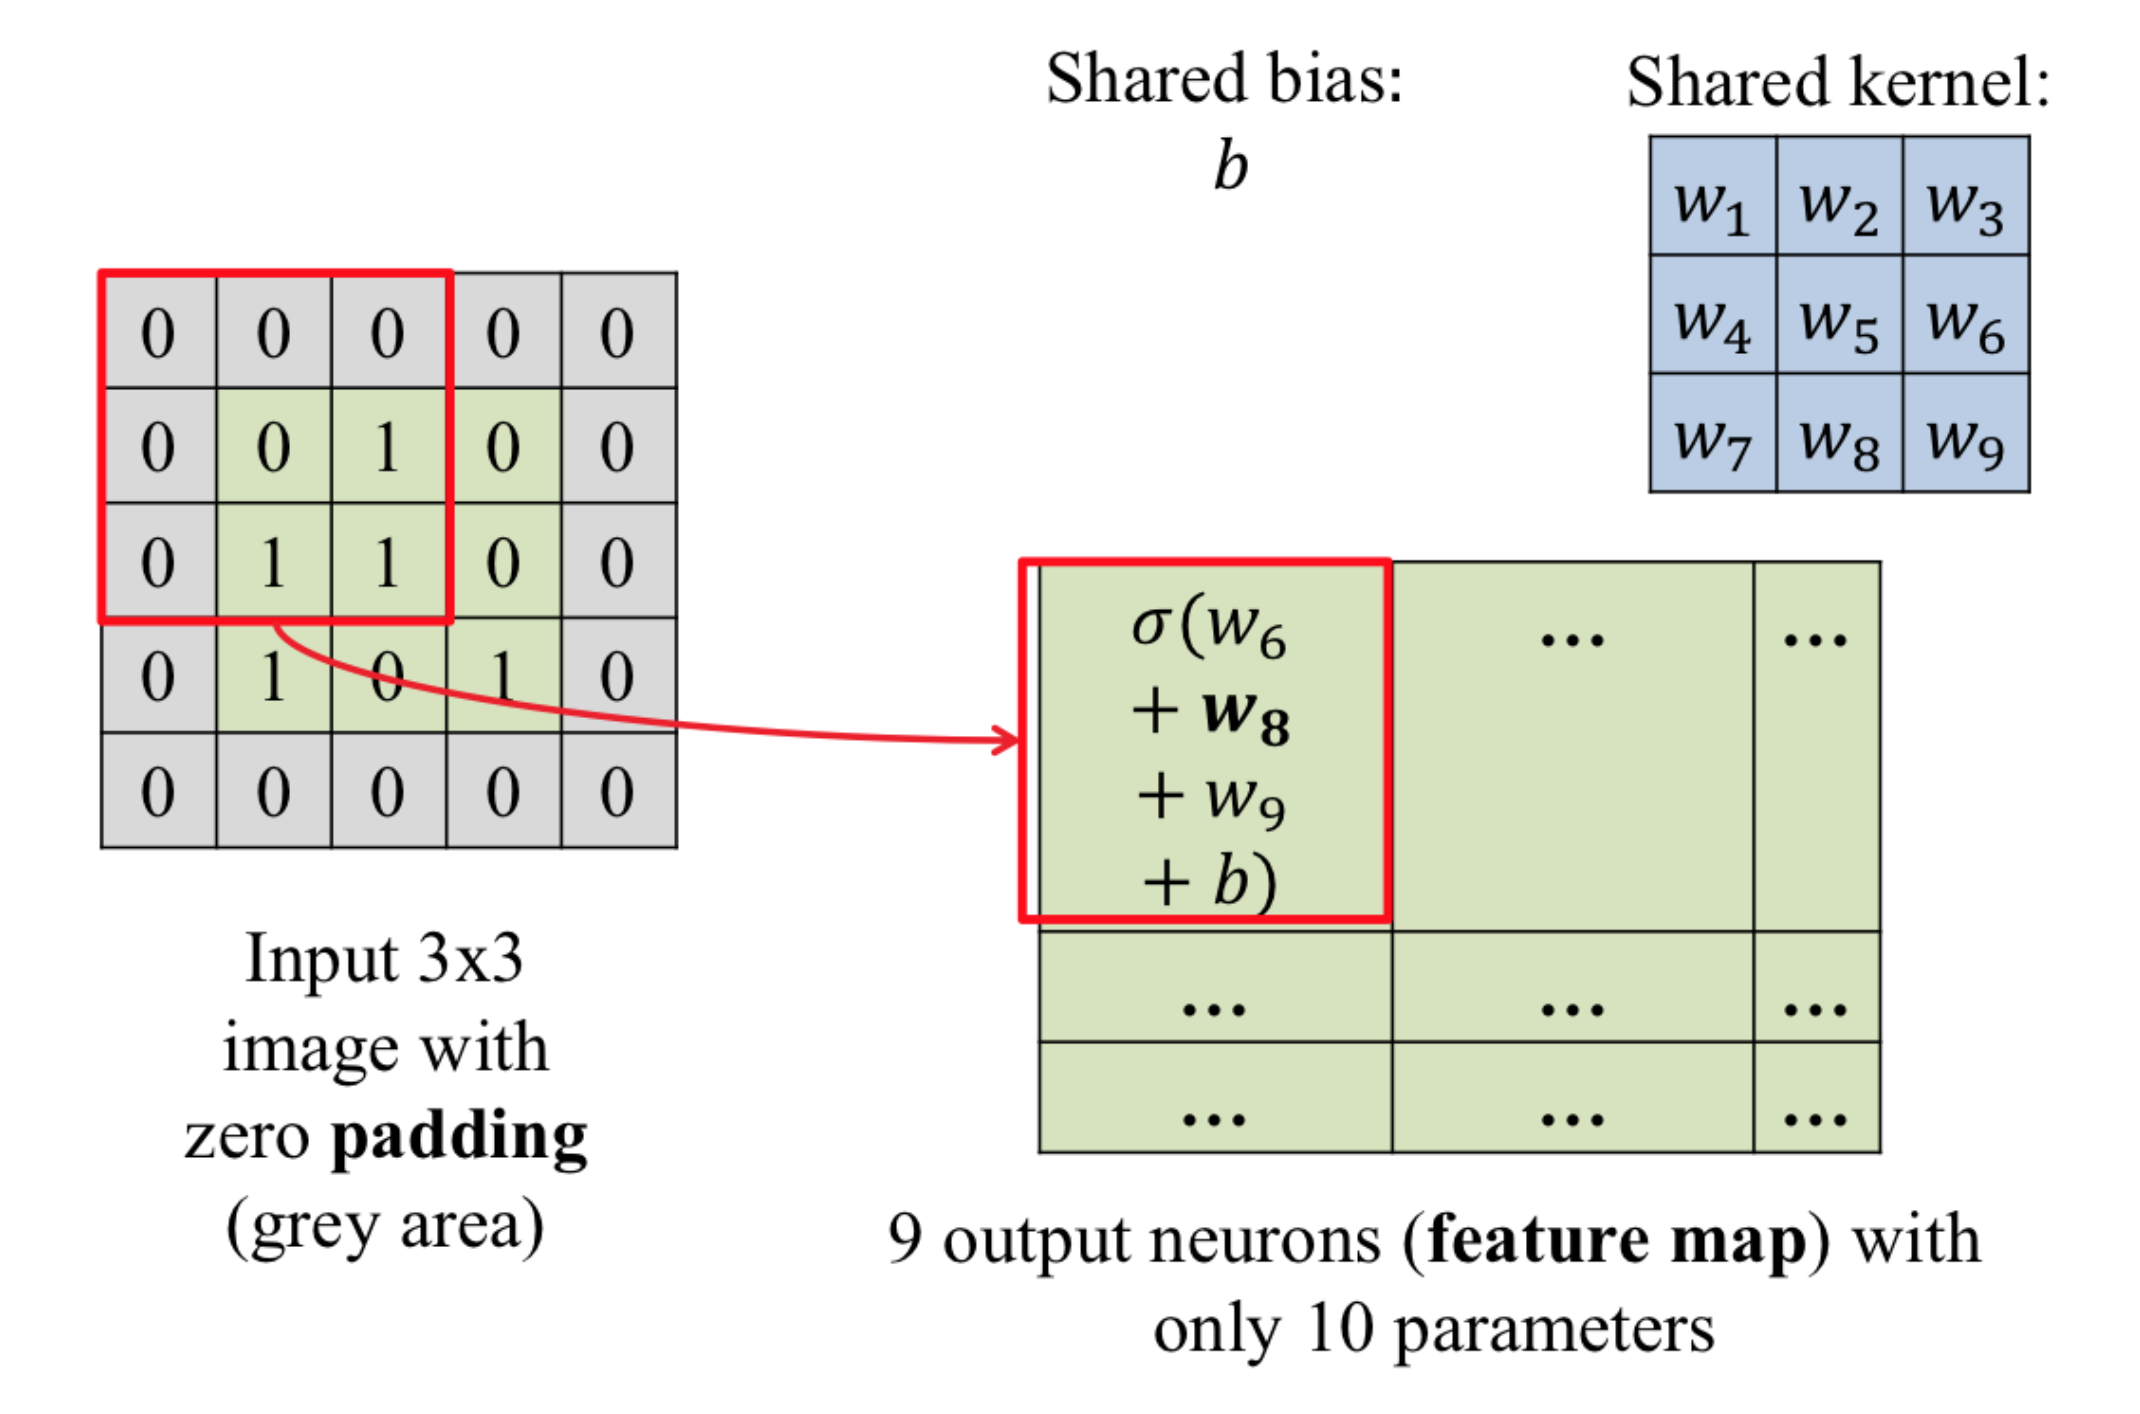
\includegraphics[width=.7\linewidth]{conv_layer.png}
\end{center}
\end{frame}


\begin{frame}{Свёрточный слой}
\begin{center}
	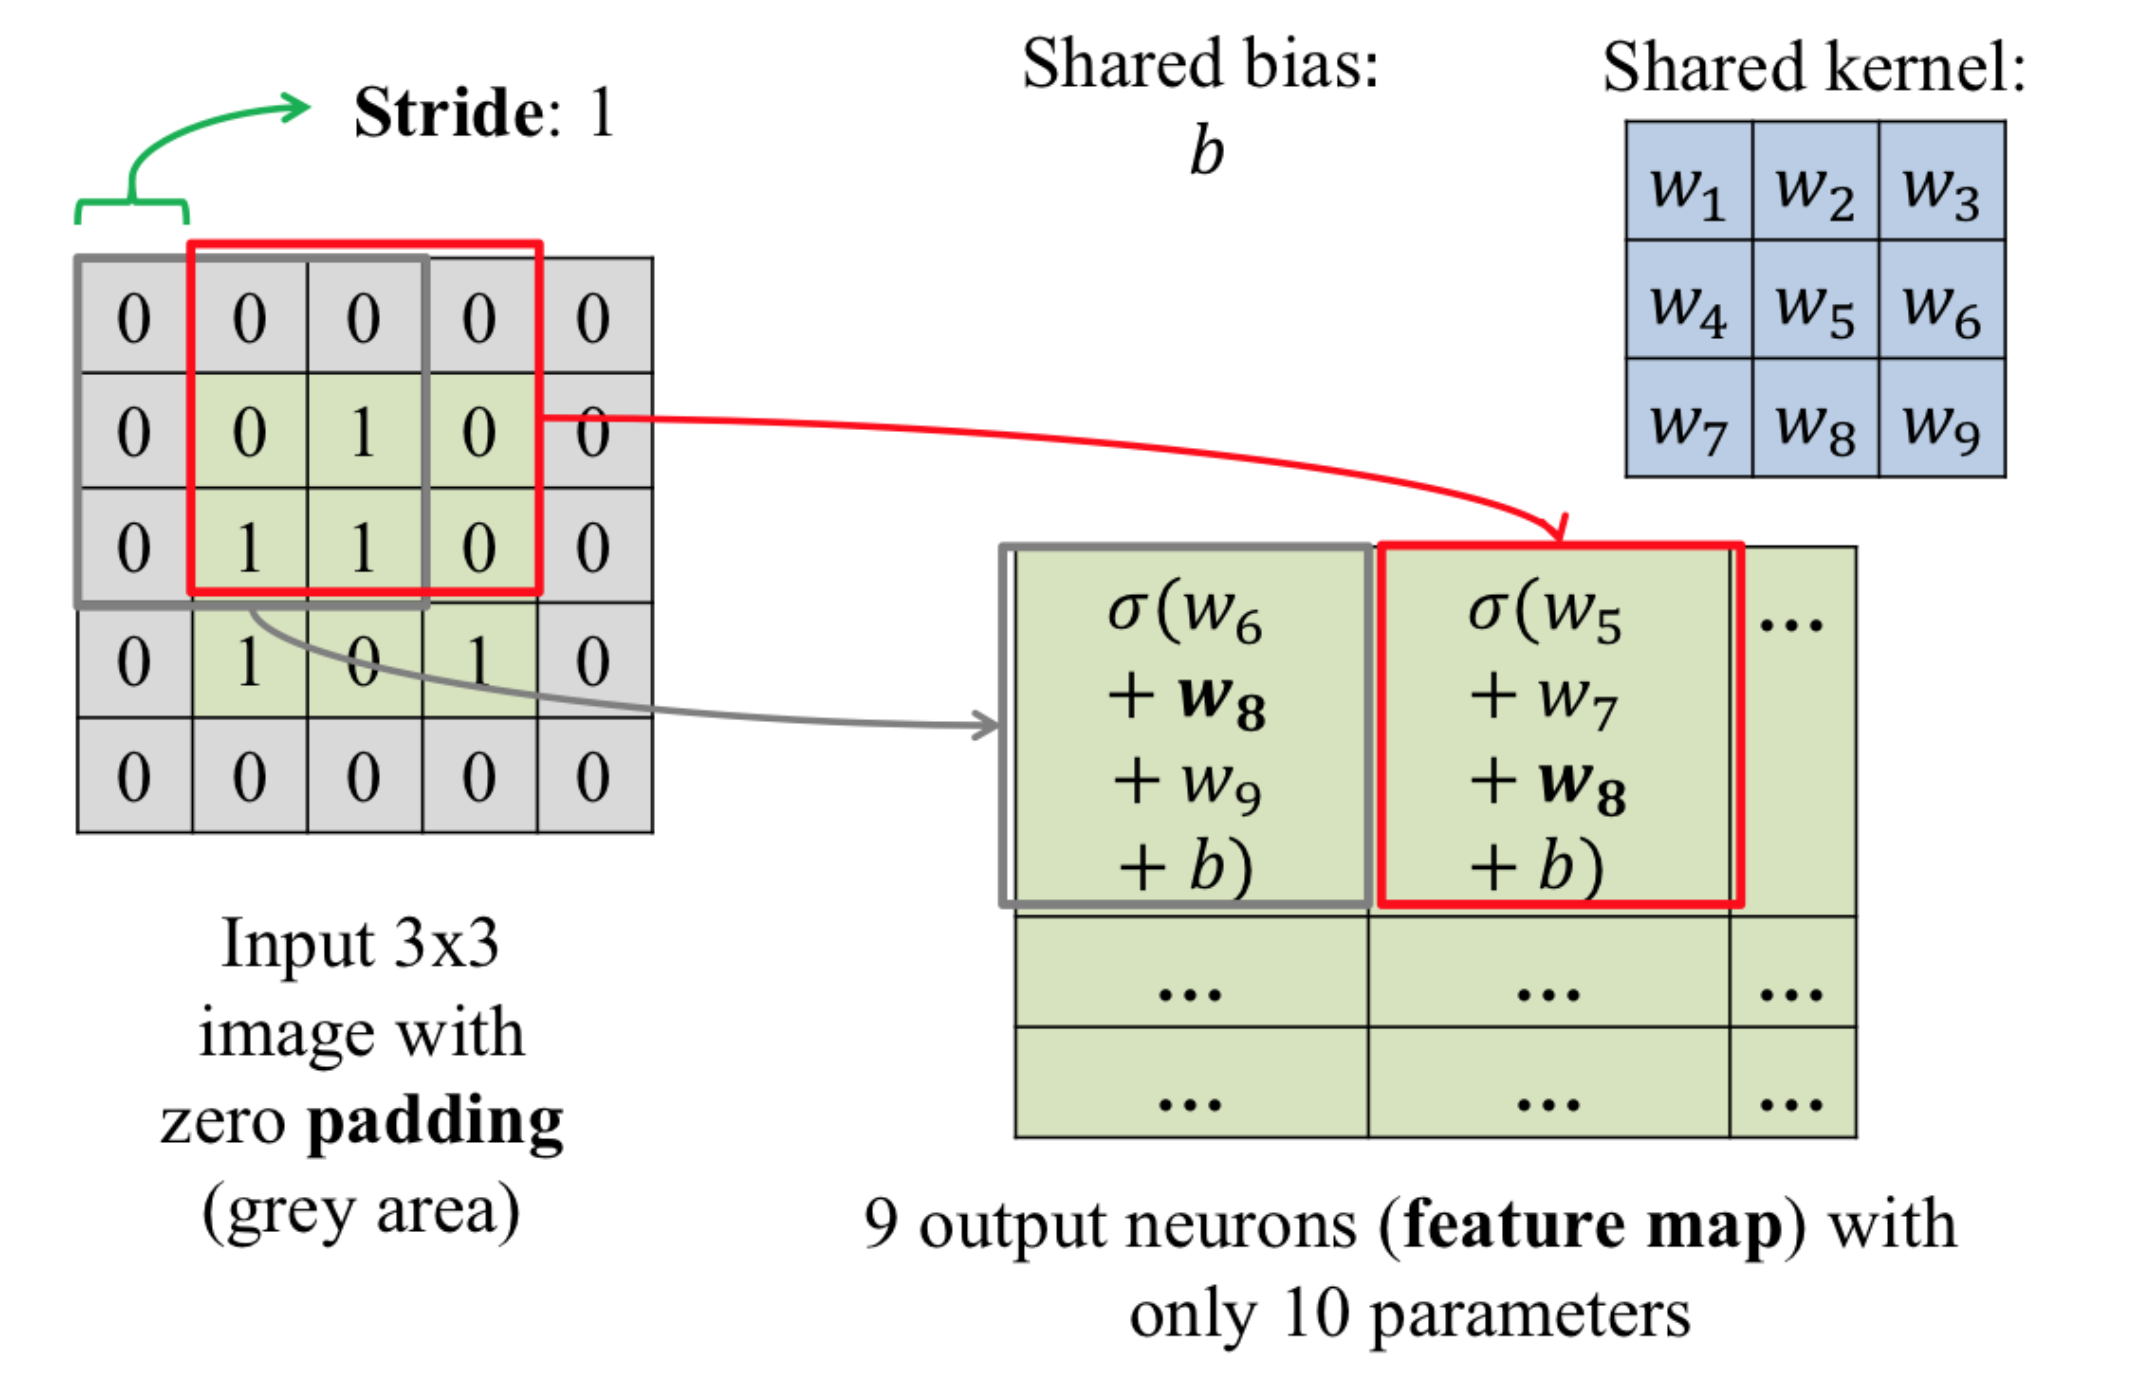
\includegraphics[width=.7\linewidth]{conv_layer_2.png}
\end{center}
\end{frame}


\begin{frame}{Backpropagation для свёрточного слоя}
\begin{center}
 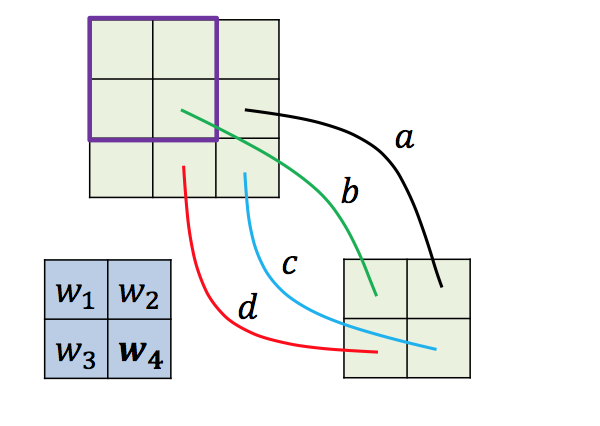
\includegraphics[width=.4\linewidth]{back_cl1.png}
\end{center}


\begin{equation*}
\begin{aligned}
& b = w_1 x_{11} + w_2 x_{12} + w_3 x_{21} + w_4 x_{22} \\
& a = w_1 x_{12} + w_2 x_{13} + w_3 x_{22} + w_4 x_{23} 
\end{aligned}
\end{equation*}
\end{frame}


\begin{frame}{Backpropagation для свёрточного слоя}
\begin{center}
	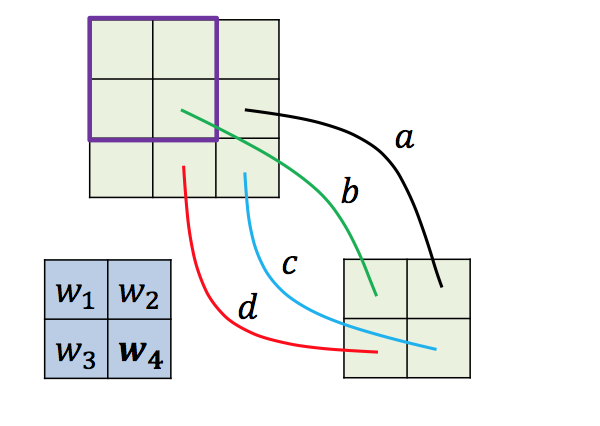
\includegraphics[width=.4\linewidth]{back_cl1.png}
\end{center}

\[
\frac{\partial L}{\partial w_1} = \frac{ \partial L }{\partial a} \cdot x_{11} + \frac{ \partial L }{\partial b} \cdot x_{12} + \frac{ \partial L }{\partial c} \cdot x_{22}  + \frac{ \partial L }{\partial d} \cdot x_{12} 
\]
\end{frame}


\begin{frame}{Свёрточный слой}
\begin{wideitemize}
	\item  Слой действует одинаково для каждого участка картинки, в отличие от полносвязного 
	\item  Нужно оценивать меньшее количество параметров
	\item  Слой учитывает взаимное расположение пикселей
	\item  Можно учить тем же самым backpropagation 
	\item  Свёрточный слой -  это полносвязный слой с ограничениями
\end{wideitemize}
\end{frame}


\begin{frame}{Одного ядра недостаточно}
\begin{center}
	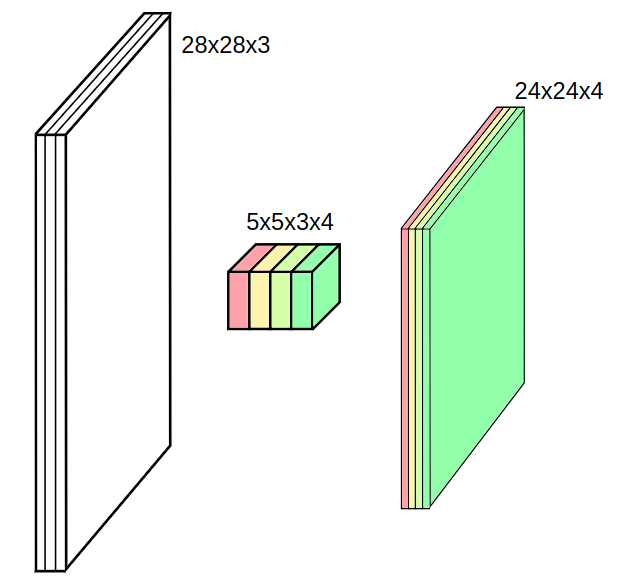
\includegraphics[width=.5\linewidth]{convolution3.png}
\end{center}
\end{frame}


\begin{frame}{Одного свёрточного слоя недостаточно}
\begin{wideitemize}
	\item  Нейроны первого слоя смотрят на поле $3 \times 3$ 
	\item  Если интересующий нас объект больше, нам нужна вторая свёртка 
\end{wideitemize}

\begin{center}
	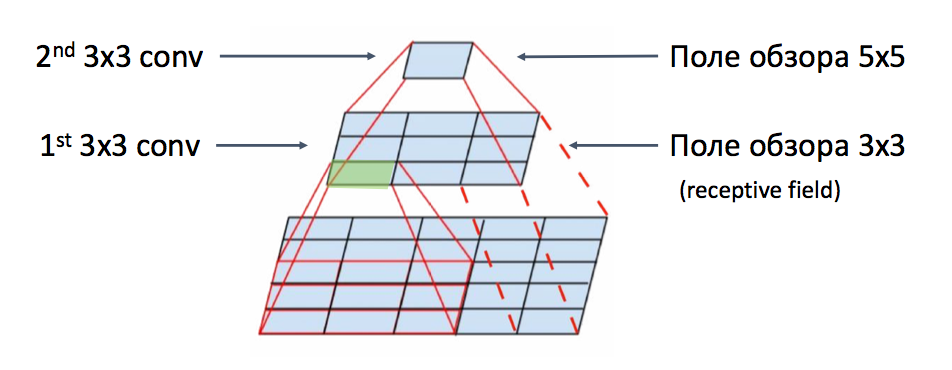
\includegraphics[width=.8\linewidth]{rec_field.png}
\end{center}
\end{frame}


\begin{frame}{Одного свёрточного слоя недостаточно}
\begin{itemize}
	\item  $N$ слоёв со свёртками $3 \times 3$ 
	\item  На $N$-ом слое поле обзора  $(2N + 1) \times (2N + 1)$
	\item  Если наш объект размера $300$, надо $150$ слоёв...  \alert{$\Rightarrow$ нужно растить поле обзора быстрее}
\end{itemize}

\begin{center}
	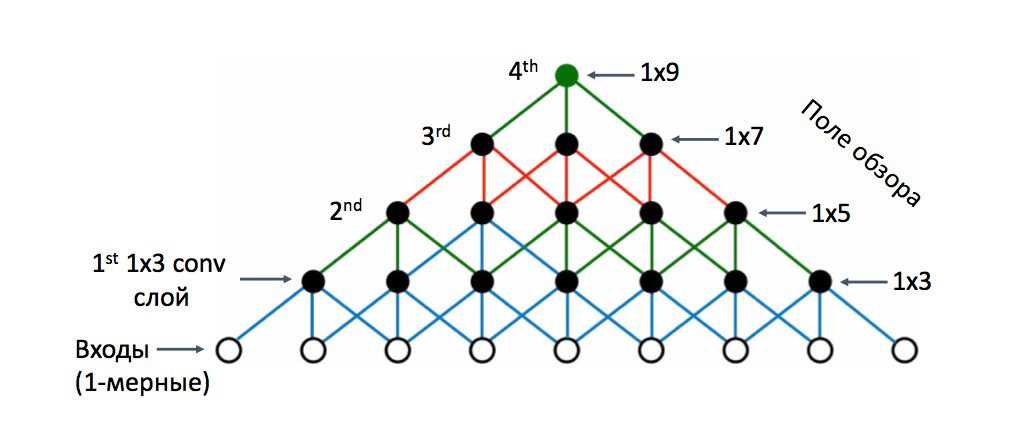
\includegraphics[width=.8\linewidth]{rec_field2.png}
\end{center}
\end{frame}


\begin{transitionframe}
	\begin{center}
		\Huge  Сдвиги и Пулинг
	\end{center}
\end{transitionframe}


\begin{frame}{Нужно растить поле обзора быстрее!}
\begin{wideitemize}
\item Пиксели локально скоррелированы — соседние пиксели, как правило, не сильно отличаются друг от друга	
\item  Если будем делать свёртку с каким-то шагом, сэкономим мощности компьютера и не потеряем в информации

\begin{center}
	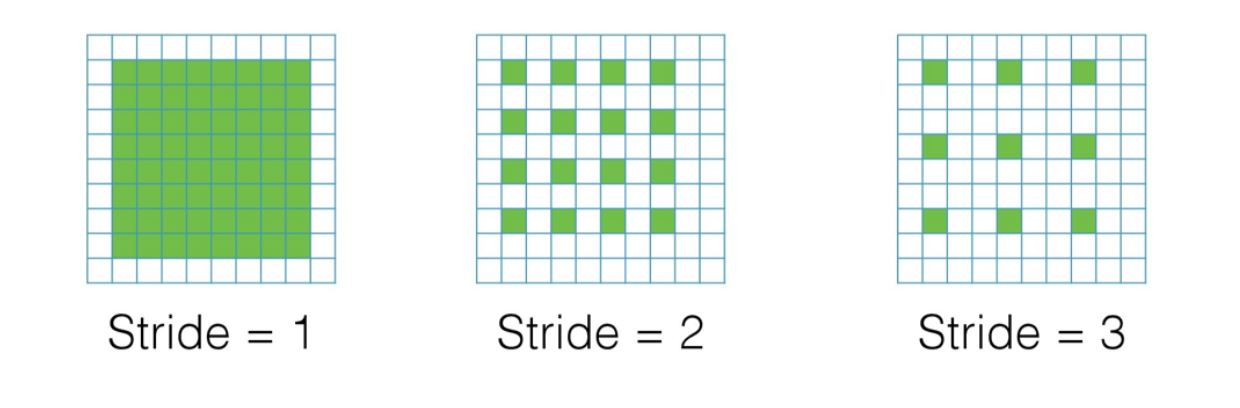
\includegraphics[width=.7\linewidth]{stride.png}
\end{center}

\item  \alert{Очень агрессивная стратегия снижения размерности картинки}
\end{wideitemize}
\end{frame}


\begin{frame}{Сдвиг (Stride)}
\begin{center}
	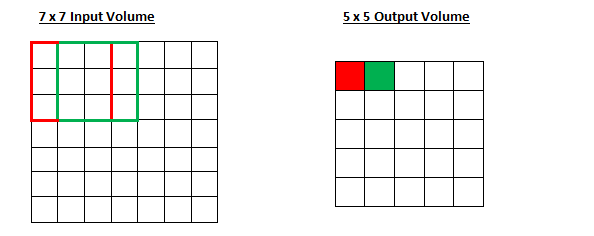
\includegraphics[width=.5\linewidth]{Stride1.png}
\end{center}
\vfill
\begin{center}
	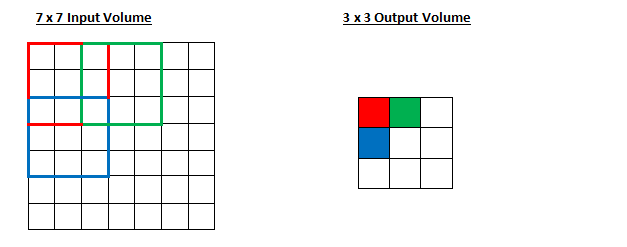
\includegraphics[width=.5\linewidth]{Stride2.png}
\end{center}
\end{frame}


\begin{frame}{Пулинг слой (Pooling)}
\begin{itemize}
	\item  Будем считать внутри какого-то окна максимум или среднее и сворачивать размерность, пользуясь локальной скоррелированностью 
\end{itemize}

\begin{center}
	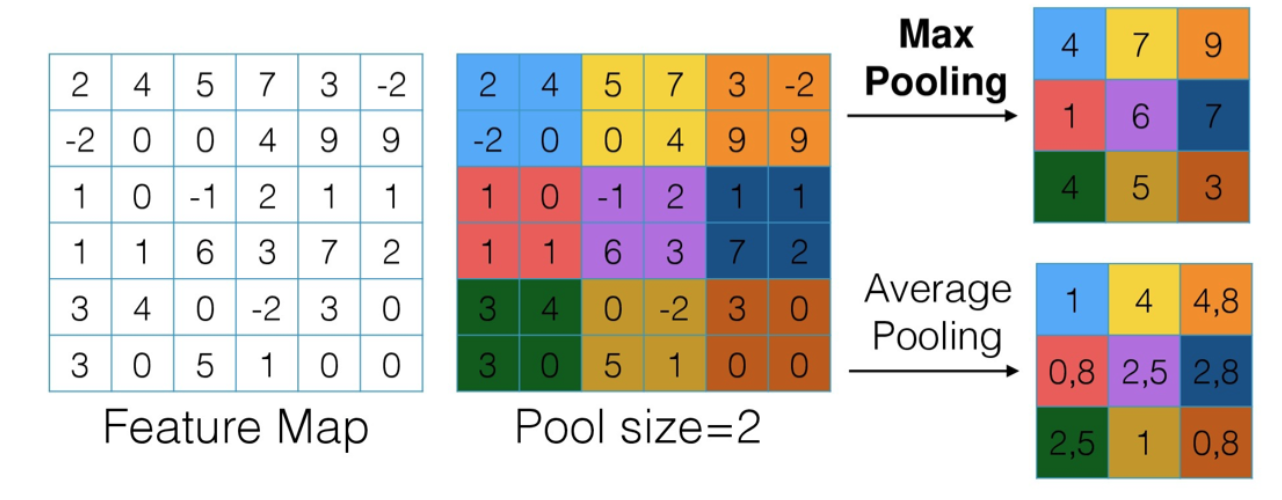
\includegraphics[width=.7\linewidth]{pooling.png}
\end{center}
\end{frame}


\begin{frame}{Простейшая CNN}
Нейросетка LeNet-5  (1998) для распознавания рукописных цифр

\begin{center}
	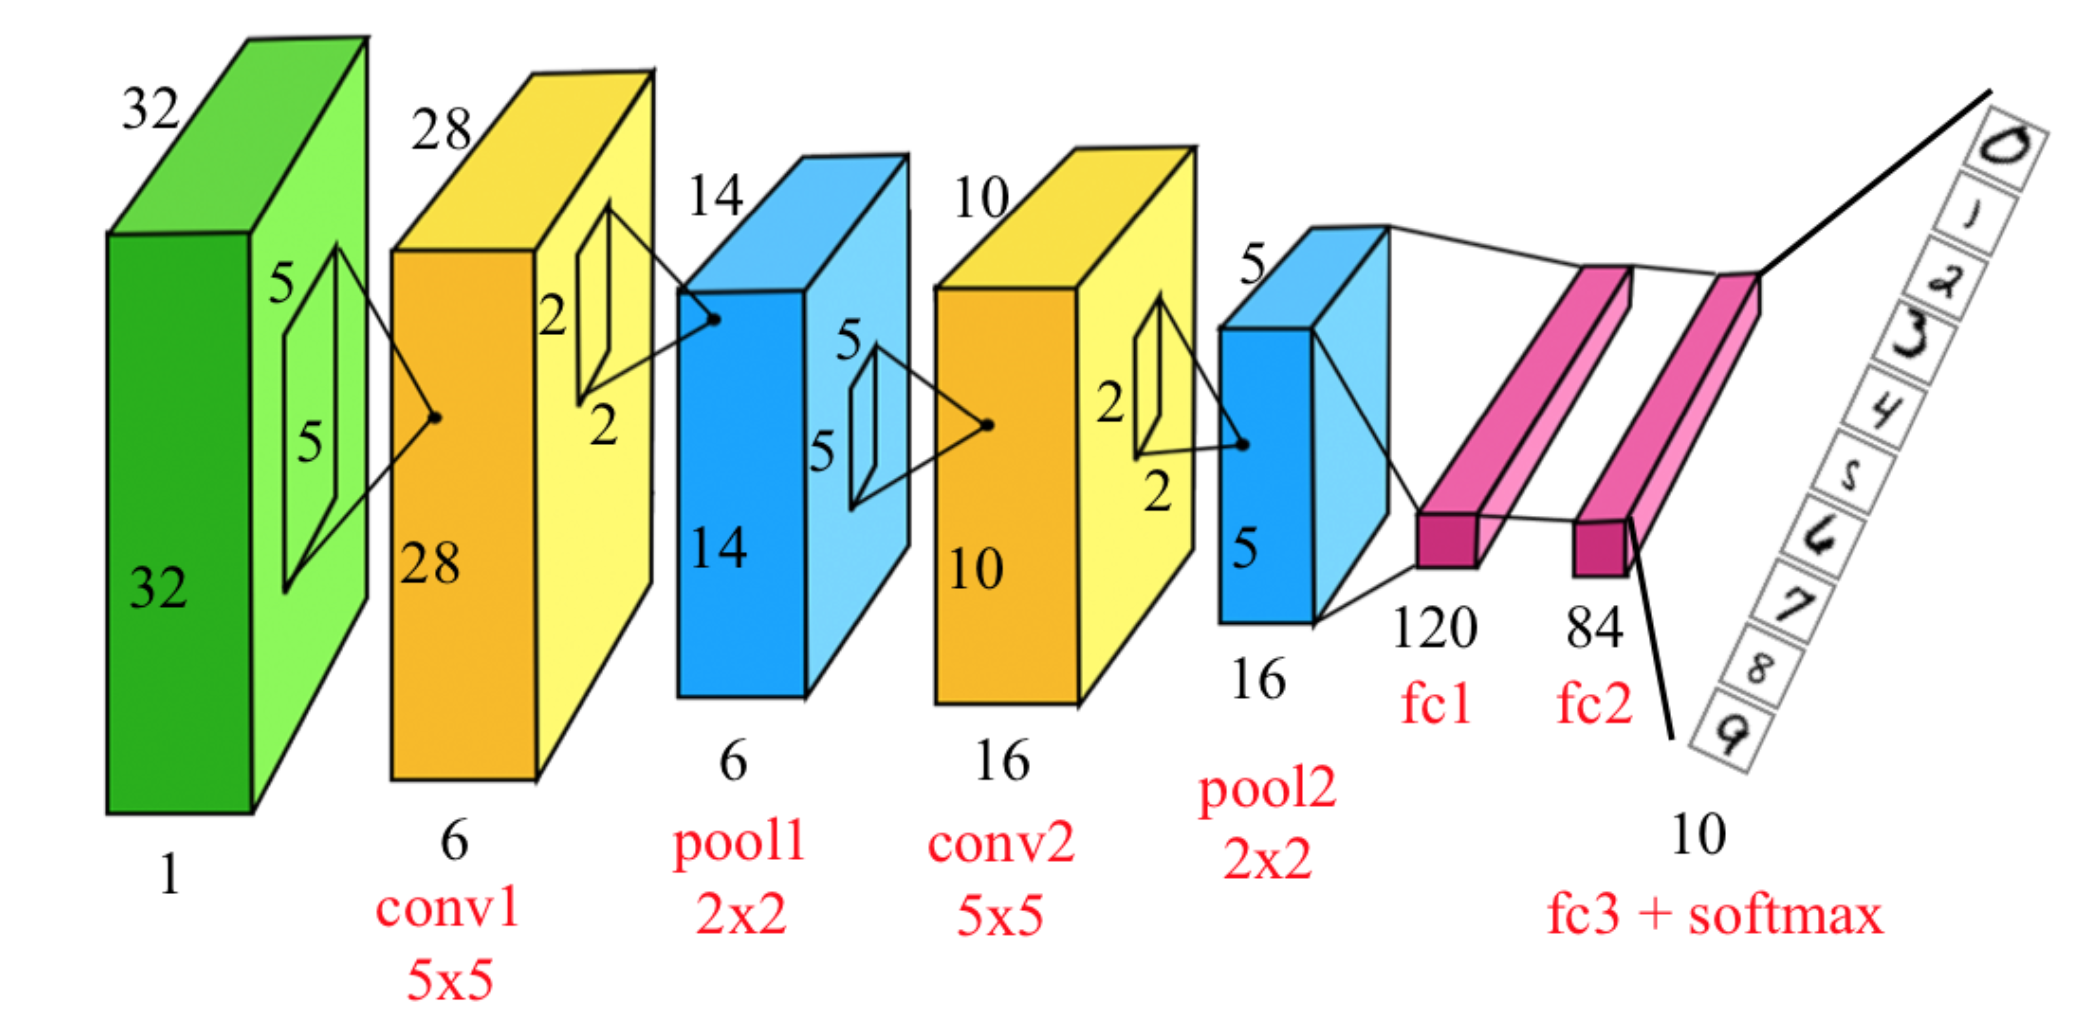
\includegraphics[width=.8\linewidth]{lenet.png}
\end{center}

\vfill
\footnotesize
{\color{blue} \url{http://yann.lecun.com/exdb/publis/pdf/lecun-98.pdf}}
\end{frame}


\begin{frame}{Что выучивают нейросети}
\begin{center}
	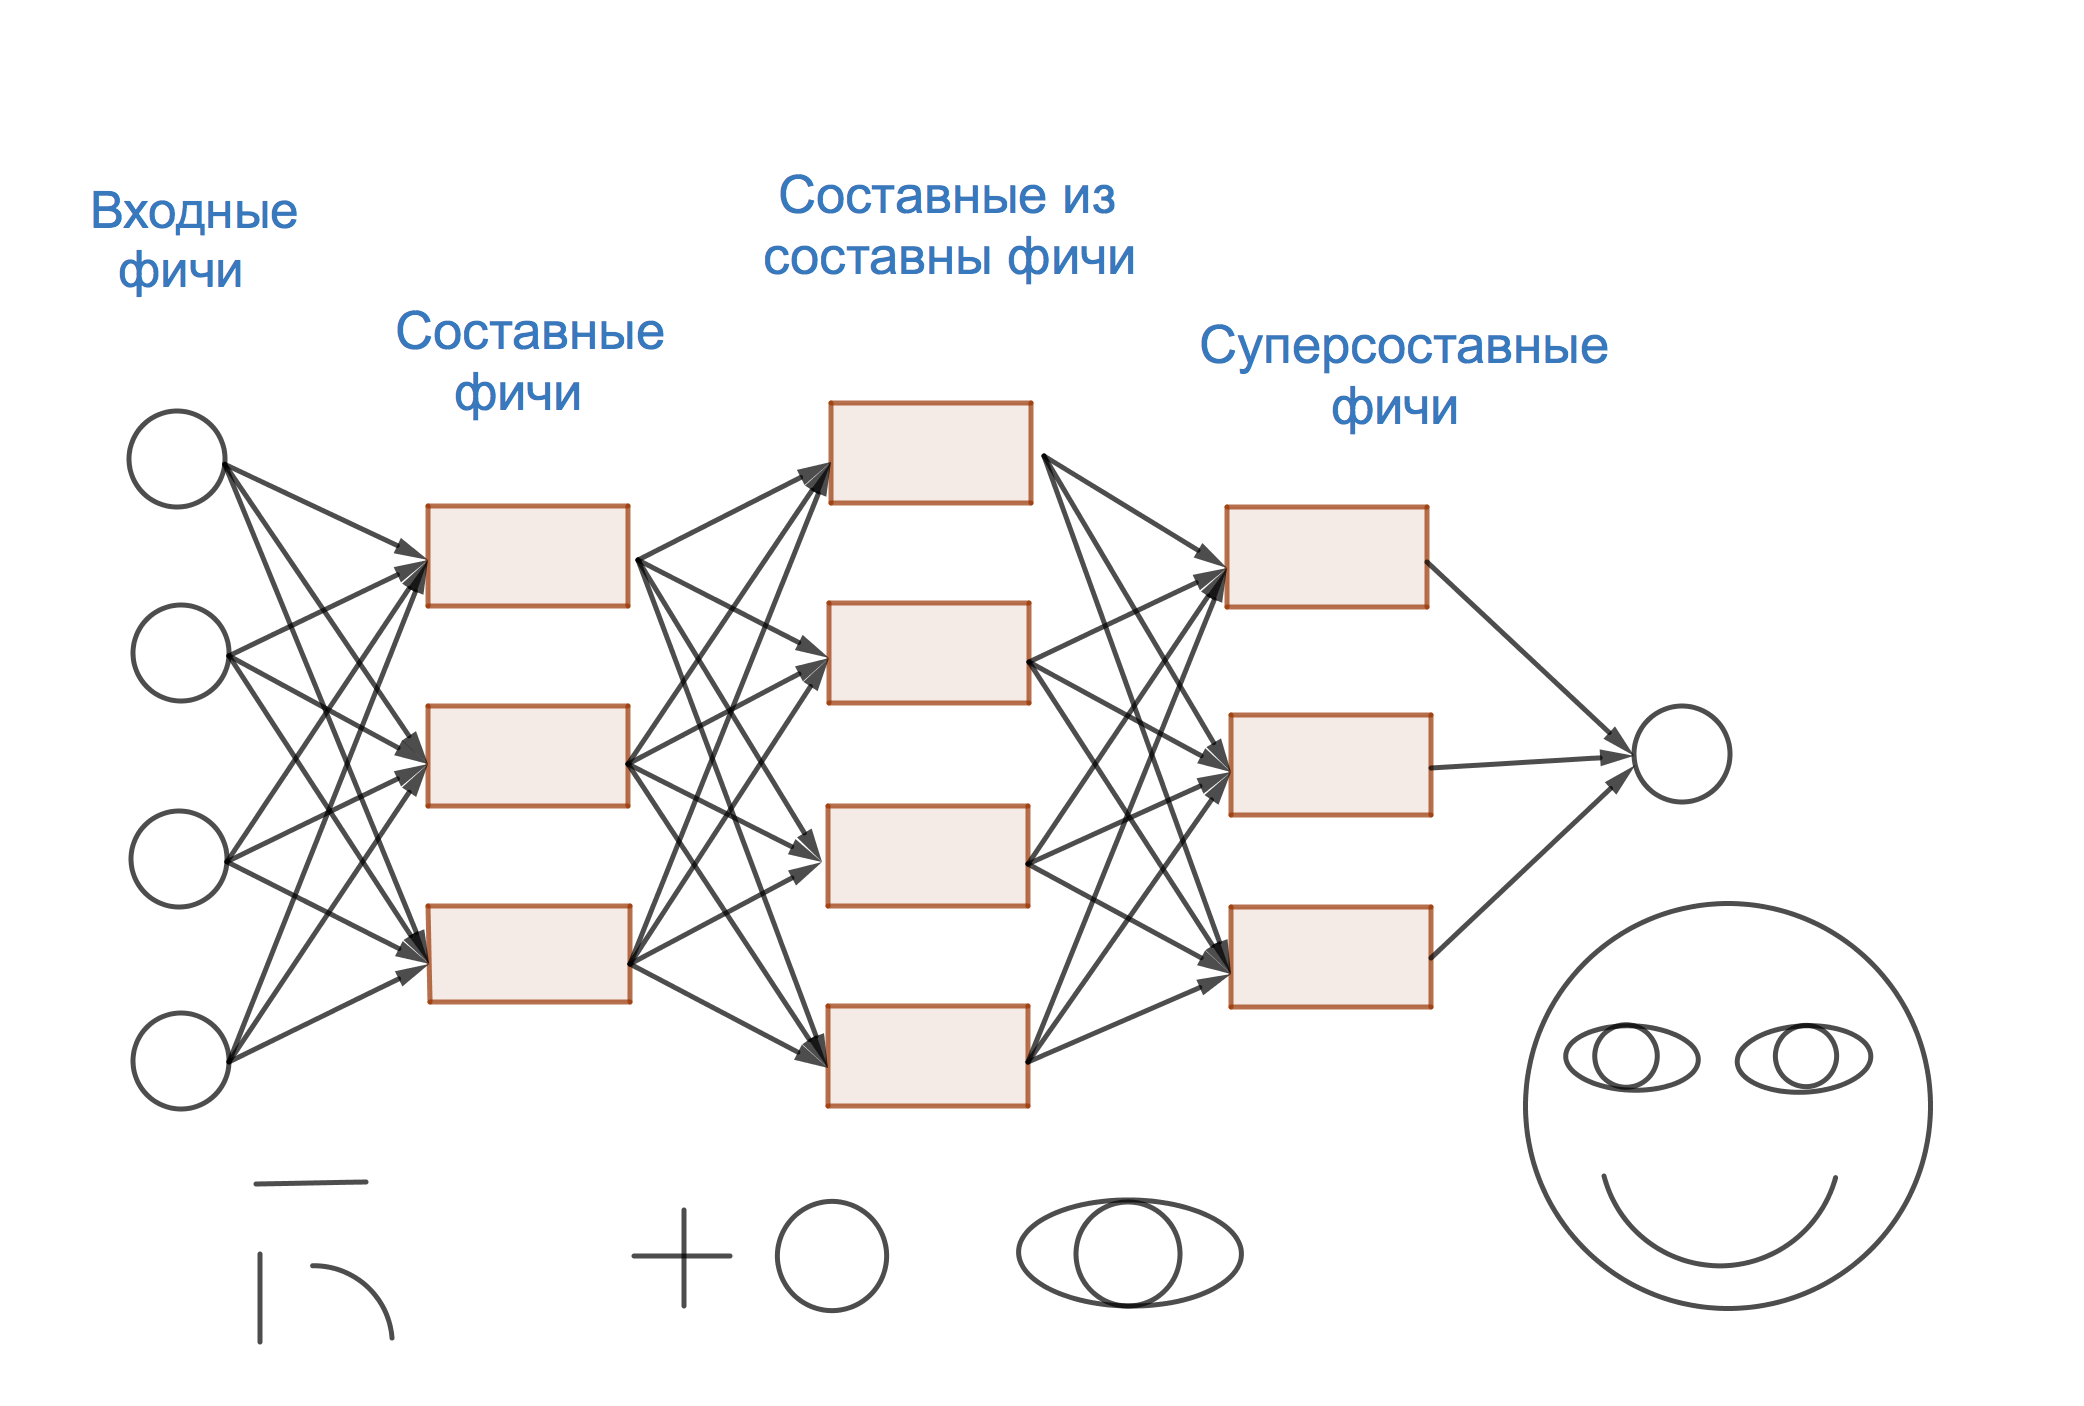
\includegraphics[width=0.73\paperwidth]{network_1.png}
\end{center}
\end{frame}


\begin{frame}{Что выучивают нейросети}
\begin{center}
	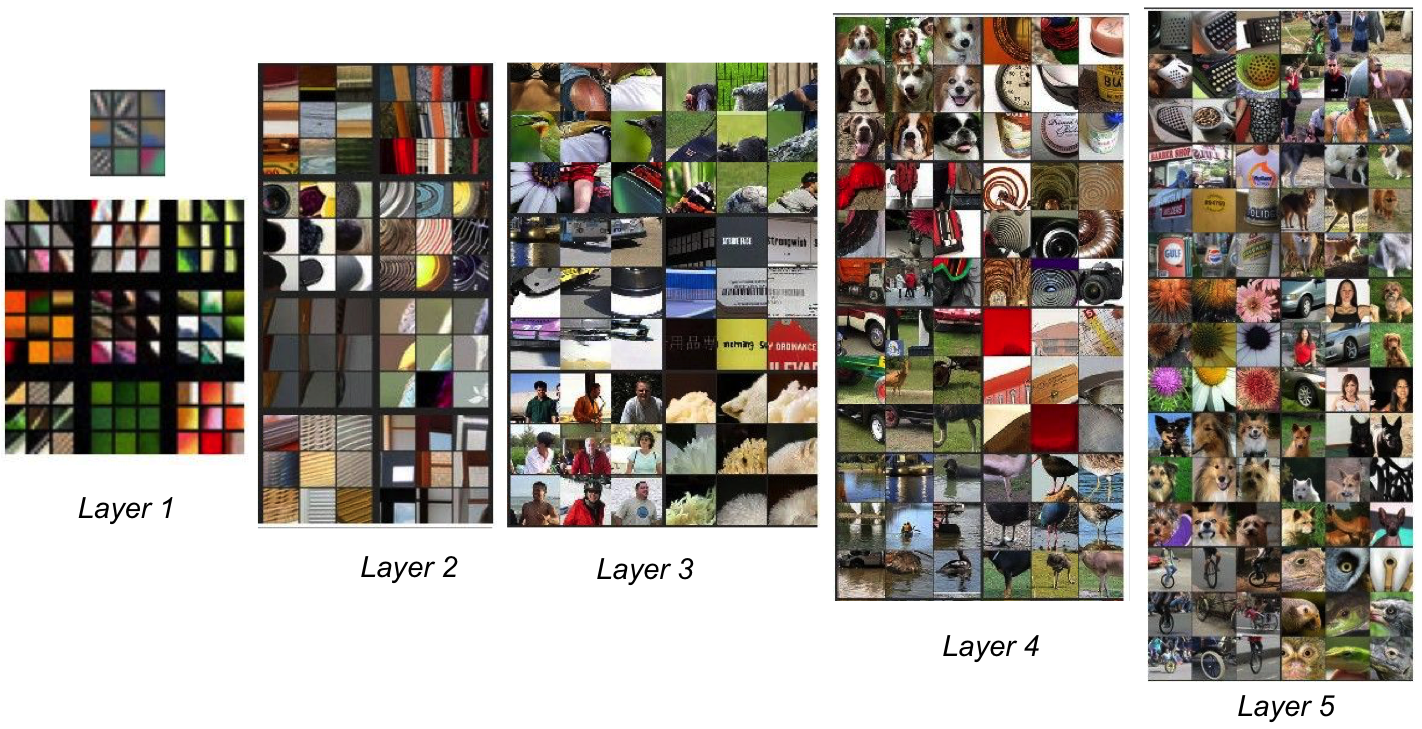
\includegraphics[width=.9\linewidth]{cnn_vis.png}
\end{center}
\vfill
\footnotesize
{\color{blue} \url{https://arxiv.org/pdf/1311.2901.pdf}}
\end{frame}


\begin{transitionframe}
	\begin{center}
		\Huge  Собираем свою собственную CNN
	\end{center}
\end{transitionframe}






%\begin{transitionframe}
%	\begin{center}
%		\Huge  Data augmentation
%	\end{center}
%\end{transitionframe}
%
%\begin{frame}{Data augmentation}
%\begin{wideitemize}
%	\item  В сетке может быть миллионы параметров!
%	\item  Естественная регуляризация, дополнительная регуляризация, генерация новых данных (data augmentation) 
%	\item Генерируем новые цвета, сдвигаем, искажаем и тп 
%\end{wideitemize}
%
%\begin{center}
%	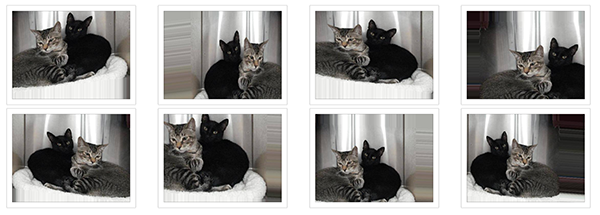
\includegraphics[width=.7\linewidth]{cat_data_augmentation.png}
%\end{center}
%
%\vfill
%\footnotesize
%{\color{blue} \url{https://blog.keras.io/building-powerful-image-classification-models-using-very-little-data.html}}
%\end{frame}
%
%
%\begin{frame}{Data augmentation}
%\begin{columns}[T] %
%	\begin{column}{.5\textwidth}
%		\begin{wideitemize}
%			\item  Сдвиги \alert{(вместо них лучше пулинг)}
%			\item Увеличение, уменьшение
%			\item Повороты
%			\item Искажение
%			\item Затенение 
%			\item Смена стиля (красок)
%		\end{wideitemize}
%	\end{column}%
%	\hfill%
%	\begin{column}{.5\textwidth}
%			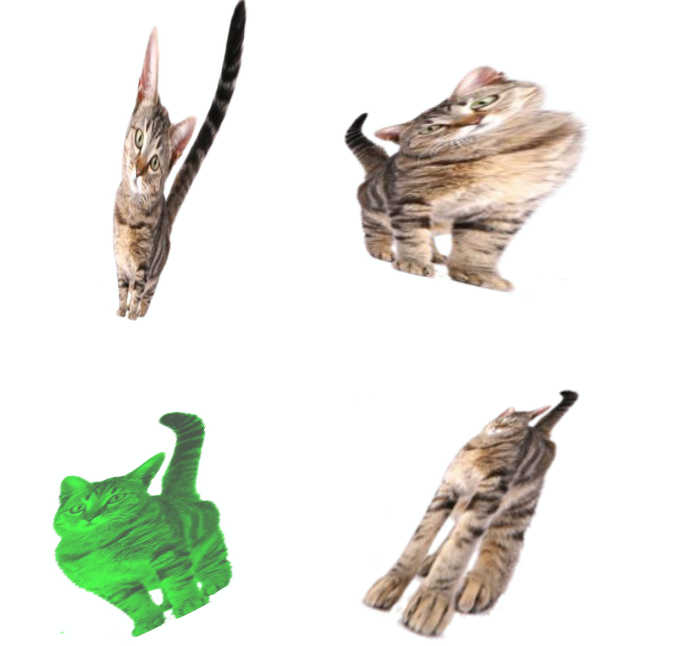
\includegraphics[scale=0.2]{still_cat.png}
%	\end{column}%
%\end{columns}
%\vfill
%\begin{center}
%Делает модель более устойчивой, полезна при маленьких выборках. На больших датасетах также улучшает результаты.
%\end{center}
%\end{frame}
%
%
%
% \begin{transitionframe}
%	\begin{center}
%		\Huge  Сказ про то как люди ImageNet рвали
%	\end{center}
%\end{transitionframe}
%
%
%\begin{frame}{ImageNet}
%\begin{wideitemize}
%	\item около 10 миллионов размеченных изображений из интернета
%\end{wideitemize}
%\begin{center}
%	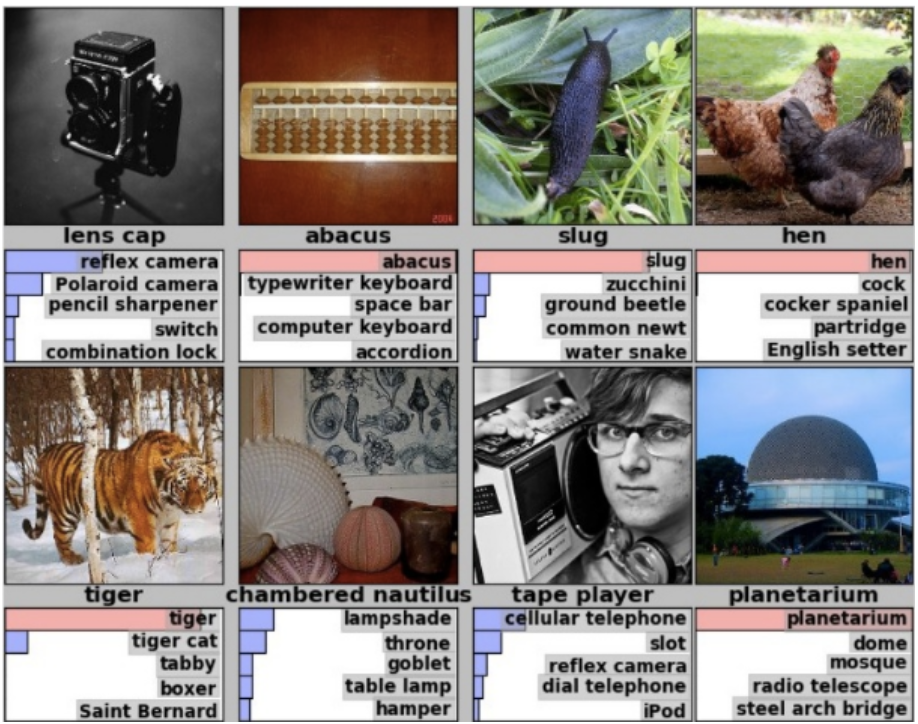
\includegraphics[width=.9\linewidth]{imagenet.png}
%\end{center}
%\vfill
%\footnotesize
%{\color{blue} \url{http://www.image-net.org/}}
%\end{frame}
%
%
%\begin{frame}{ImageNet}
%\begin{wideitemize}
%	\item  выборка очень большая и неоднородная, постоянно пополняется, соревнования на ней проводятся каждый год
%	
%	\item обычно изображение требуется отнести к одному из $1000$ классов, можно давать несколько ответов
%	
%	\item если один из пяти вариантов оказался верным, то классификация считается верной
%	
%	\item до $2012$ года лучшие алгоритмы дают ошибку в $25\%$
%	
%	\item в $2012$ году на арену выходят глубокие нейронные сети
%\end{wideitemize}
%\end{frame}
%
%
%\begin{frame}{ImageNet}
%\begin{wideitemize}
%	\item бывают спорные изображения: тут вишня, если распознать как далматинец, будет неправильно 
%	
%	\begin{center}
%		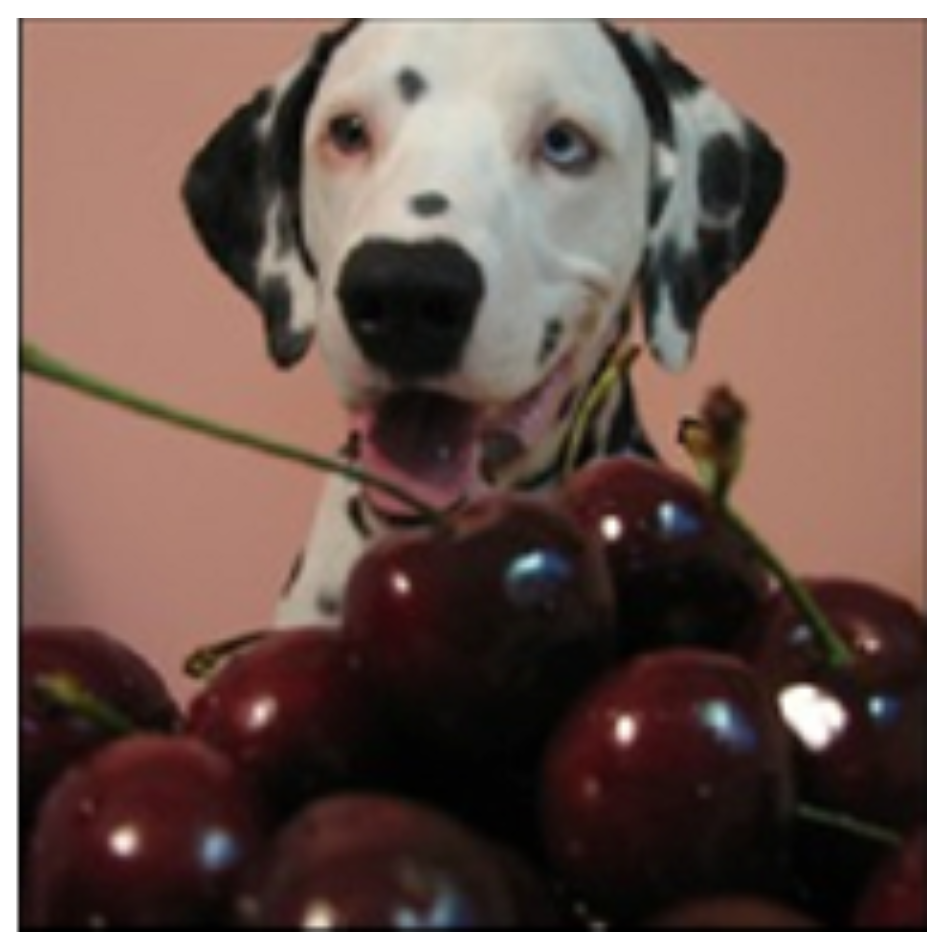
\includegraphics[width=.27\linewidth]{dog_vish.png}
%	\end{center}
%	
%	\item Можно попробовать сразиться с компьютером:  {\color{blue} \url{https://cs.stanford.edu/people/karpathy/ilsvrc/}} 
%\end{wideitemize}
%\end{frame}
%
%
%\begin{frame}{Точность сетей на ImageNet}
%\begin{center}
%	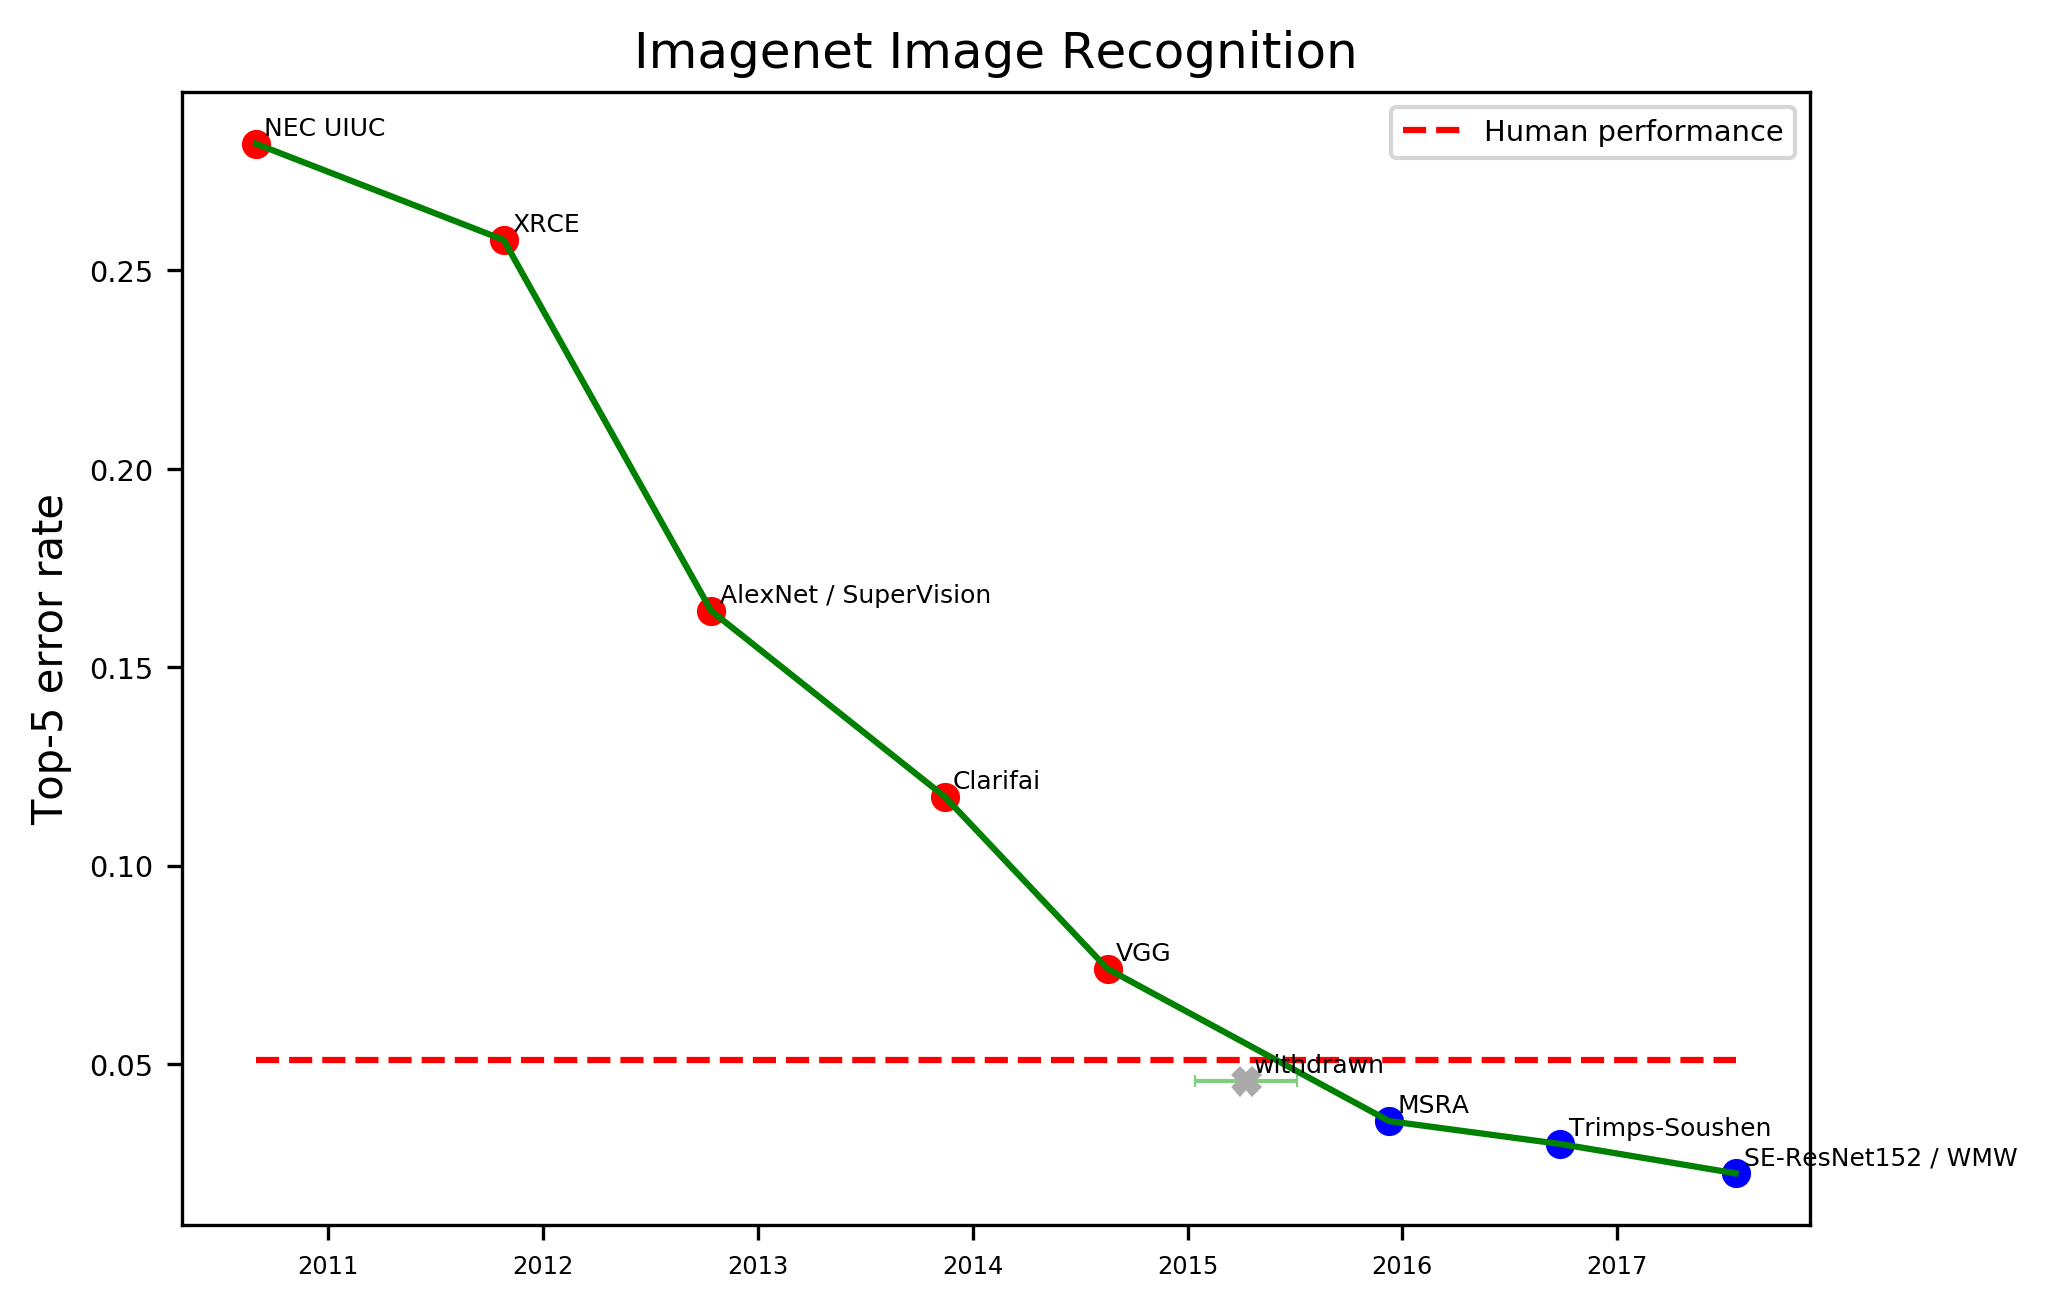
\includegraphics[width=.7\linewidth]{imagenet_recognition.png}
%\end{center}
%\vfill %
%\footnotesize
%\color{blue} \url{https://www.eff.org/ai/metrics}
%\end{frame} 
%
%
%\begin{frame}{AlexNet (2012)}
%\begin{center}
%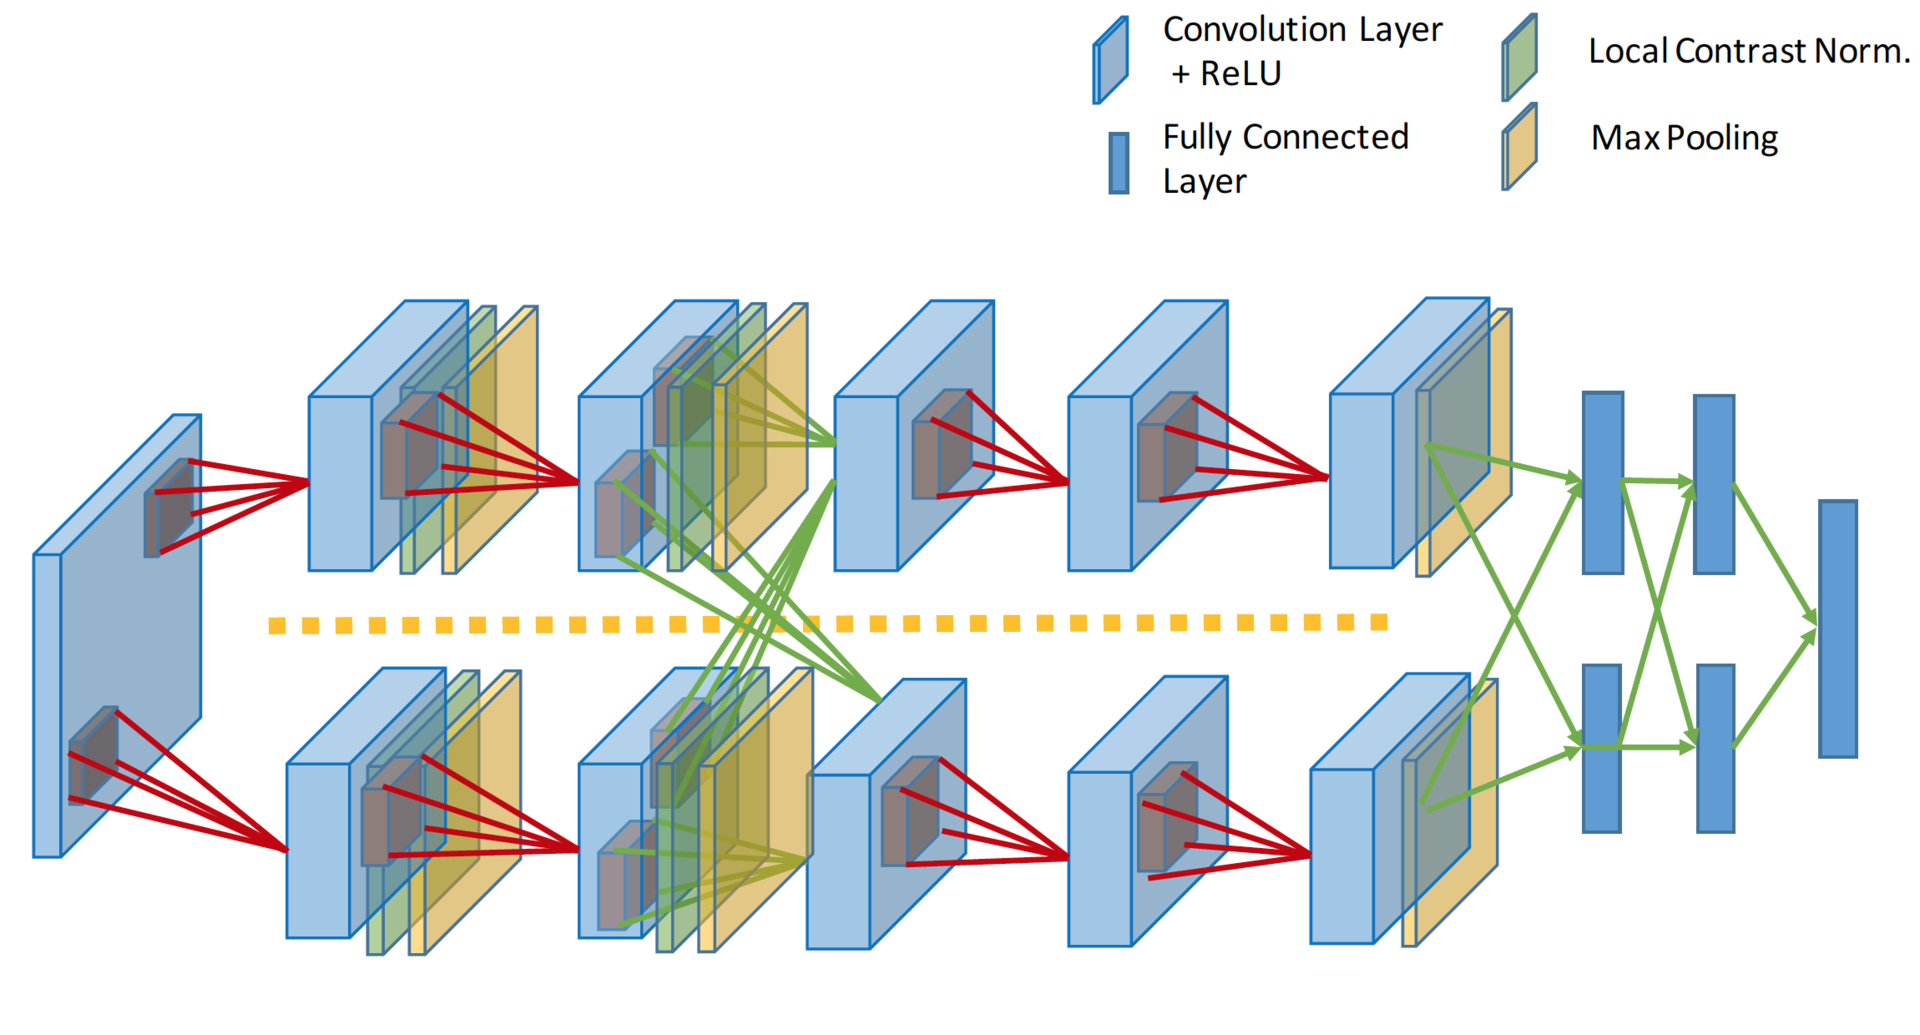
\includegraphics[width=.9\linewidth]{alexnet.png}
%\end{center}
%\vfill %
%\tiny
%\color{blue} \url{https://papers.nips.cc/paper/4824-imagenet-classification-with-deep-convolutional-neural-networks.pdf}
%\end{frame}
%
%
%\begin{frame}{AlexNet (2012)}
%\begin{wideitemize}
%	\item Тот же LeNet из 1998г. но увеличен в $1000$ раз и дополненный трюками (Dropout, ReLU, Data augmentation) 
%	\item Свёртки $11 \times 11$, $5 \times 5$, $3 \times 3$
%	\item  Уронила ошибку с $25\%$ до $15.4\%$ 
%	\item  $60$ миллионов параметров 
%	\item  Училась $6$ дней на $2$ GPU 
%	\item Попробовали сделать ансамблю из таких сеток, ошибка упала до $11.7\%$
%\end{wideitemize}
%\end{frame}
%
%
%\begin{frame}{VGG (2014)}
%\begin{center}
%	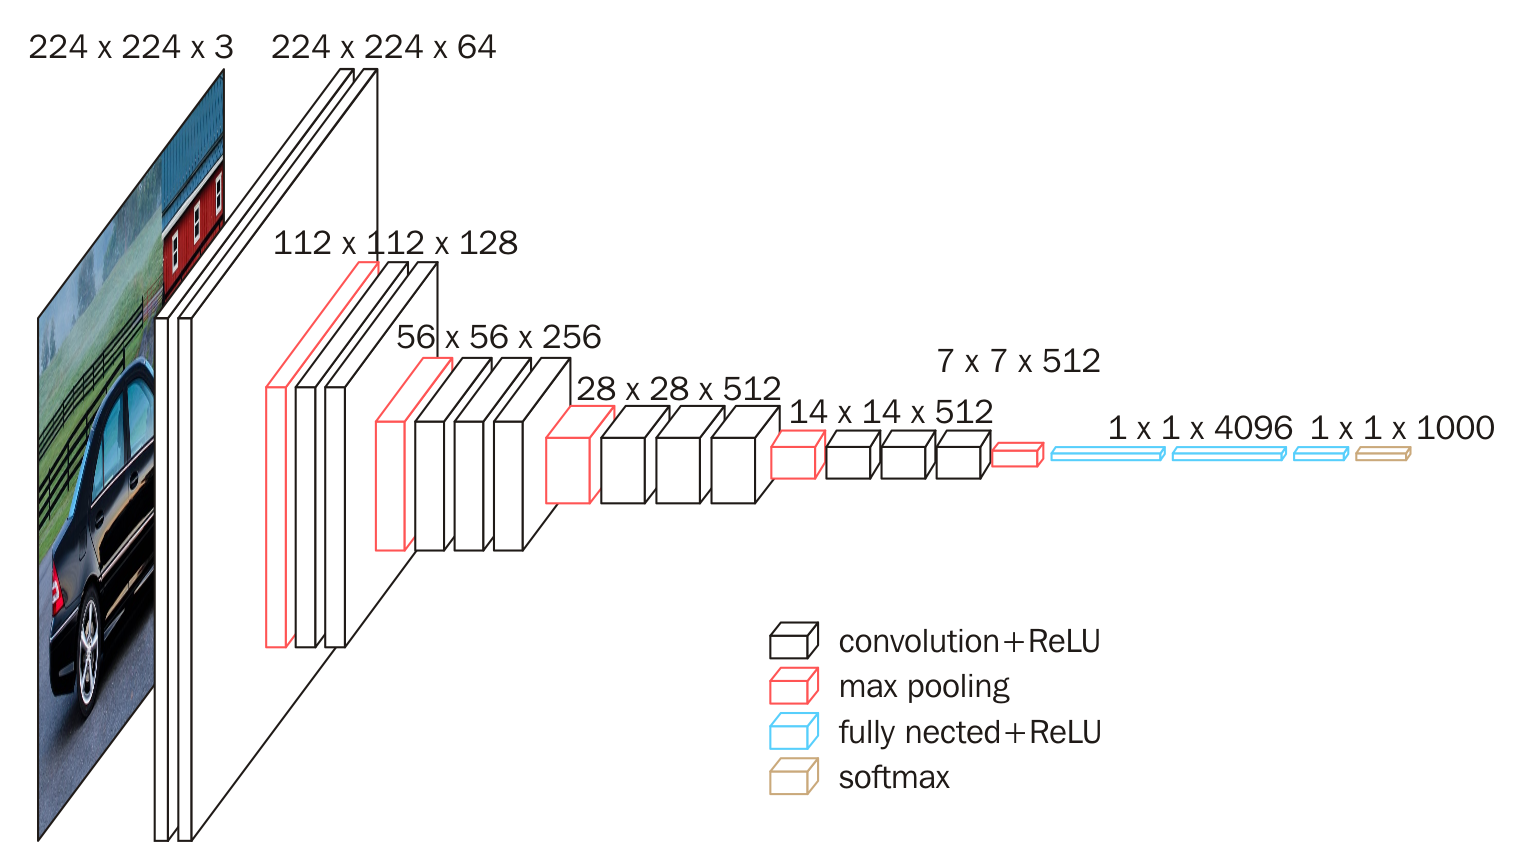
\includegraphics[width=.7\linewidth]{vgg.png}
%\end{center}
%\vfill %
%\footnotesize
%\color{blue} \url{https://www.datalearner.com/paper_note/content/300035}
%\end{frame}
%
%
%\begin{frame}{VGG (2014)}
%\begin{wideitemize}
%	\item  $138$ миллионов параметров
%	\item  Училась $2-3$ недели на $4$ GPU 
%	\item Ошибка упала до $6.8\%$
%	\item Свёртки только $3 \times 3$, но намного больше фильтров для экономии параметров (две свёртки $3\times 3$ покрывают поле $5 \times 5$ и требуют $18$ параметров, а свёртка $5 \times 5$ требует $25$ параметров)
%	\begin{center}
%		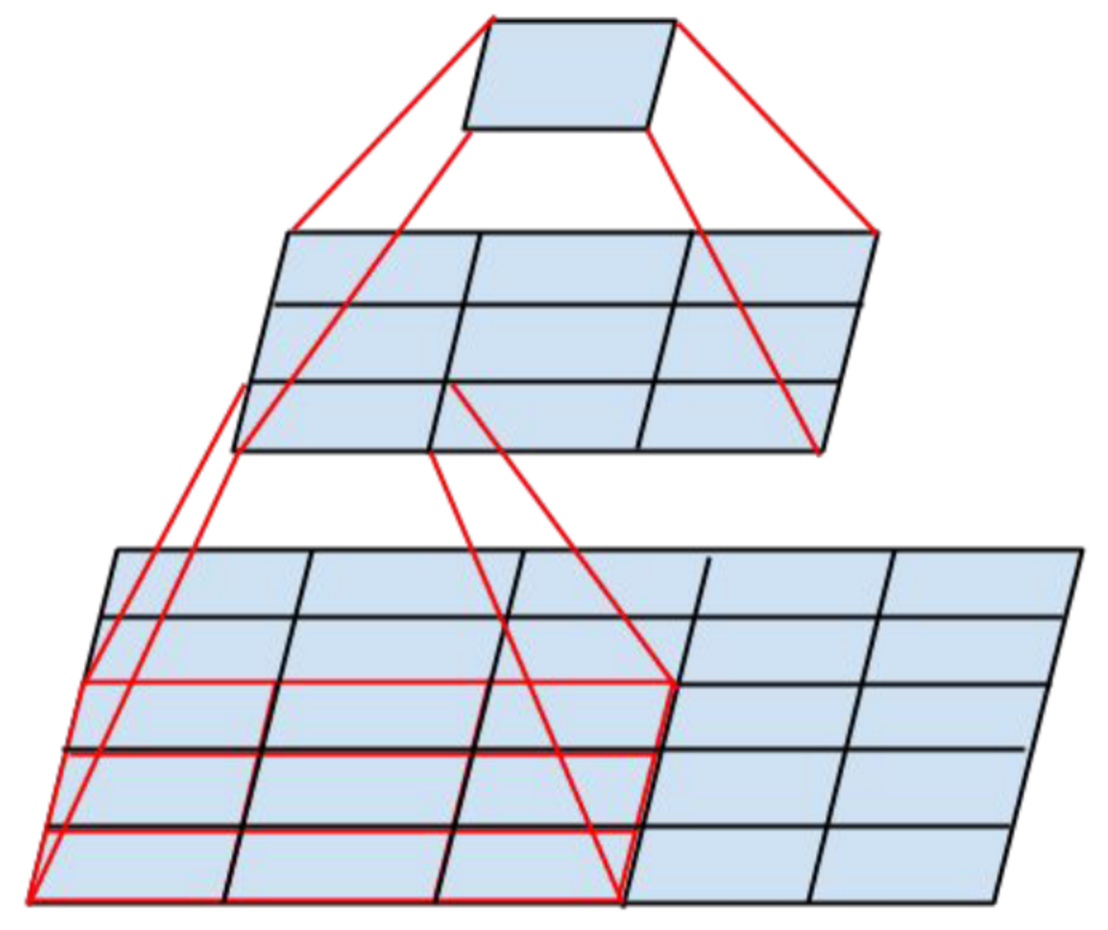
\includegraphics[width=.2\linewidth]{vgg_conv.png}
%	\end{center}
%\end{wideitemize}
%\end{frame}
%
%
%\begin{frame}{GoogleLeNet aka Inception V1  (2014)}
%	\begin{center}
%		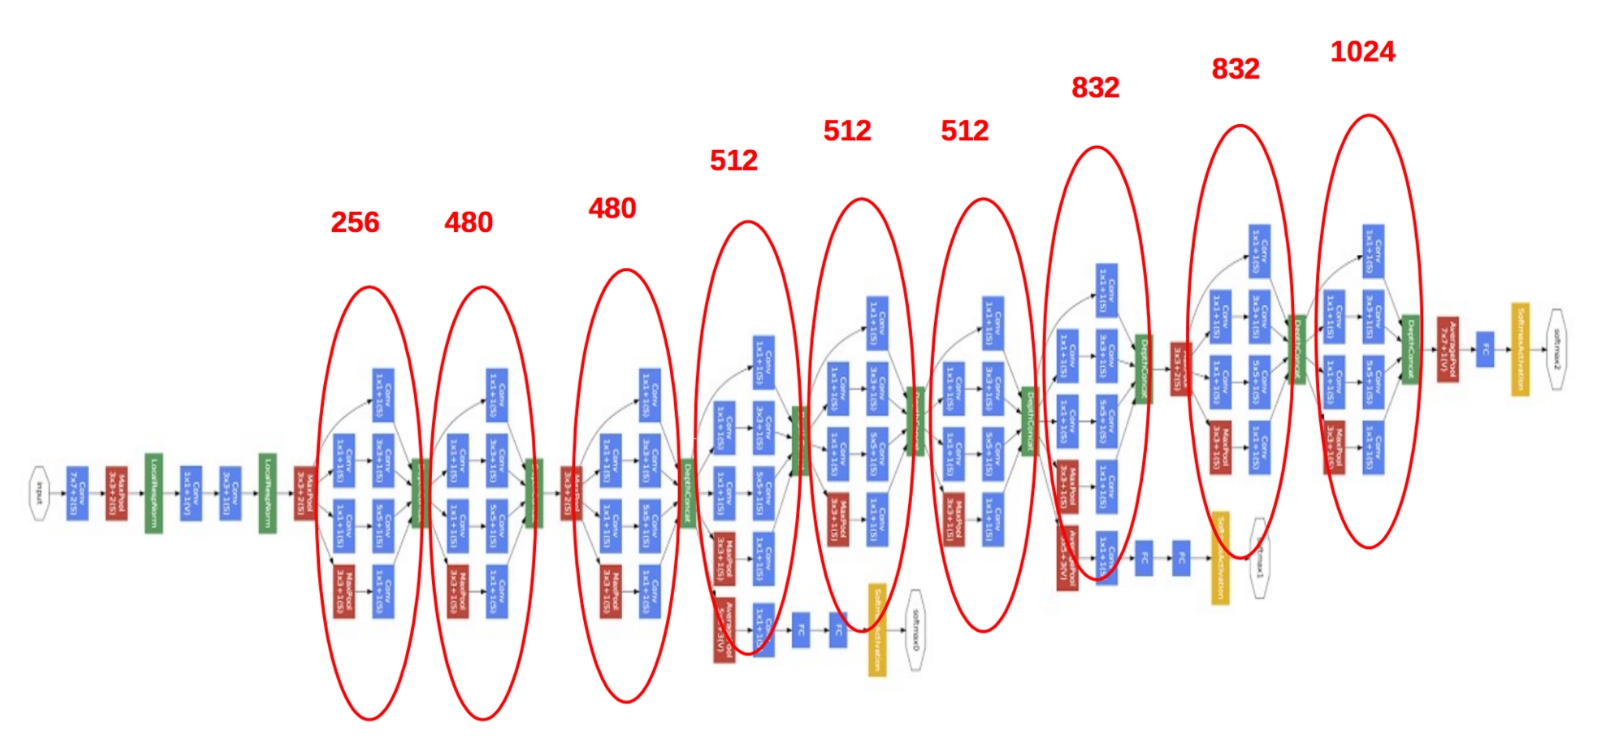
\includegraphics[width=.95\linewidth]{inception.png}
%	\end{center}
%\vfill %
%\footnotesize
%\color{blue} \url{https://arxiv.org/abs/1409.4842}
%\end{frame}
%
%
%\begin{frame}{GoogleLeNet aka Inception V1}
%\begin{center}
%	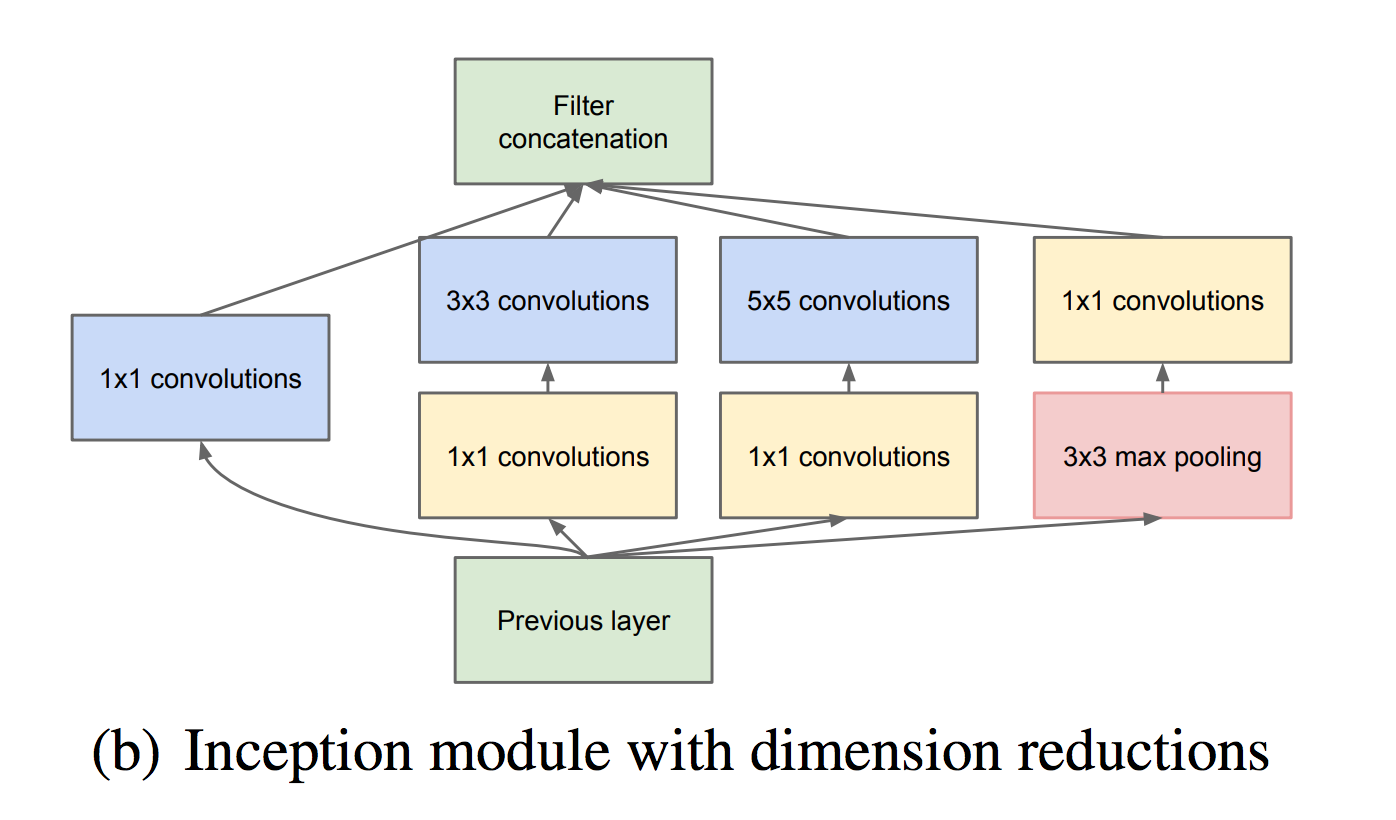
\includegraphics[width=.7\linewidth]{inception_module.png}
%\end{center}
%\end{frame}
%
%
%\begin{frame}{GoogleLeNet aka Inception V1  (2014)}
%\begin{wideitemize}
%	\item  Парни из Google решили усовершенствовать AlexNet.
%	
%	\item  Уменьшаем свёртки, саму \alert{сетку собираем из компонент}  (всего 9 блоков).
%	
%	\item  На каждом слое используется ни одна свёртка, а несколько разных, что помогает реагировать на сигналы разного масштаба и улучшает работу, используются  \alert{свёртки $1 \times 1$.}
%	
%	\item \alert{Несколько дополнительных классификаторов на разных уровнях.} Идея в том, что такие классификаторы позволят «протолкнуть» градиенты к ранним слоям и тем самым уменьшить эффект затухания градиента.
%	
%	\item  Параметров  в $10$ раз меньше, чем в AlexNet, работает лучше, $6.7\%$ ошибок 
%\end{wideitemize}
%\end{frame}
%
%
%\begin{frame}{Свёртка $1 \times 1$}
%\begin{columns}[T] %
%	\begin{column}{.4\textwidth}
%			\begin{wideitemize}
%				\item  Позволяет сократить размерность по числу каналов
%				\item  Представляет из себя полносвязный слой по фильтрам 
%				\item  В Inception мы делаем много разных свёрток, а потом свёрткой $1 \times 1$ выбираем из них лучшее, агрессивно понижая размерность
%			\end{wideitemize}
%	\end{column}%
%	\hfill%
%	\begin{column}{.6\textwidth}
%		 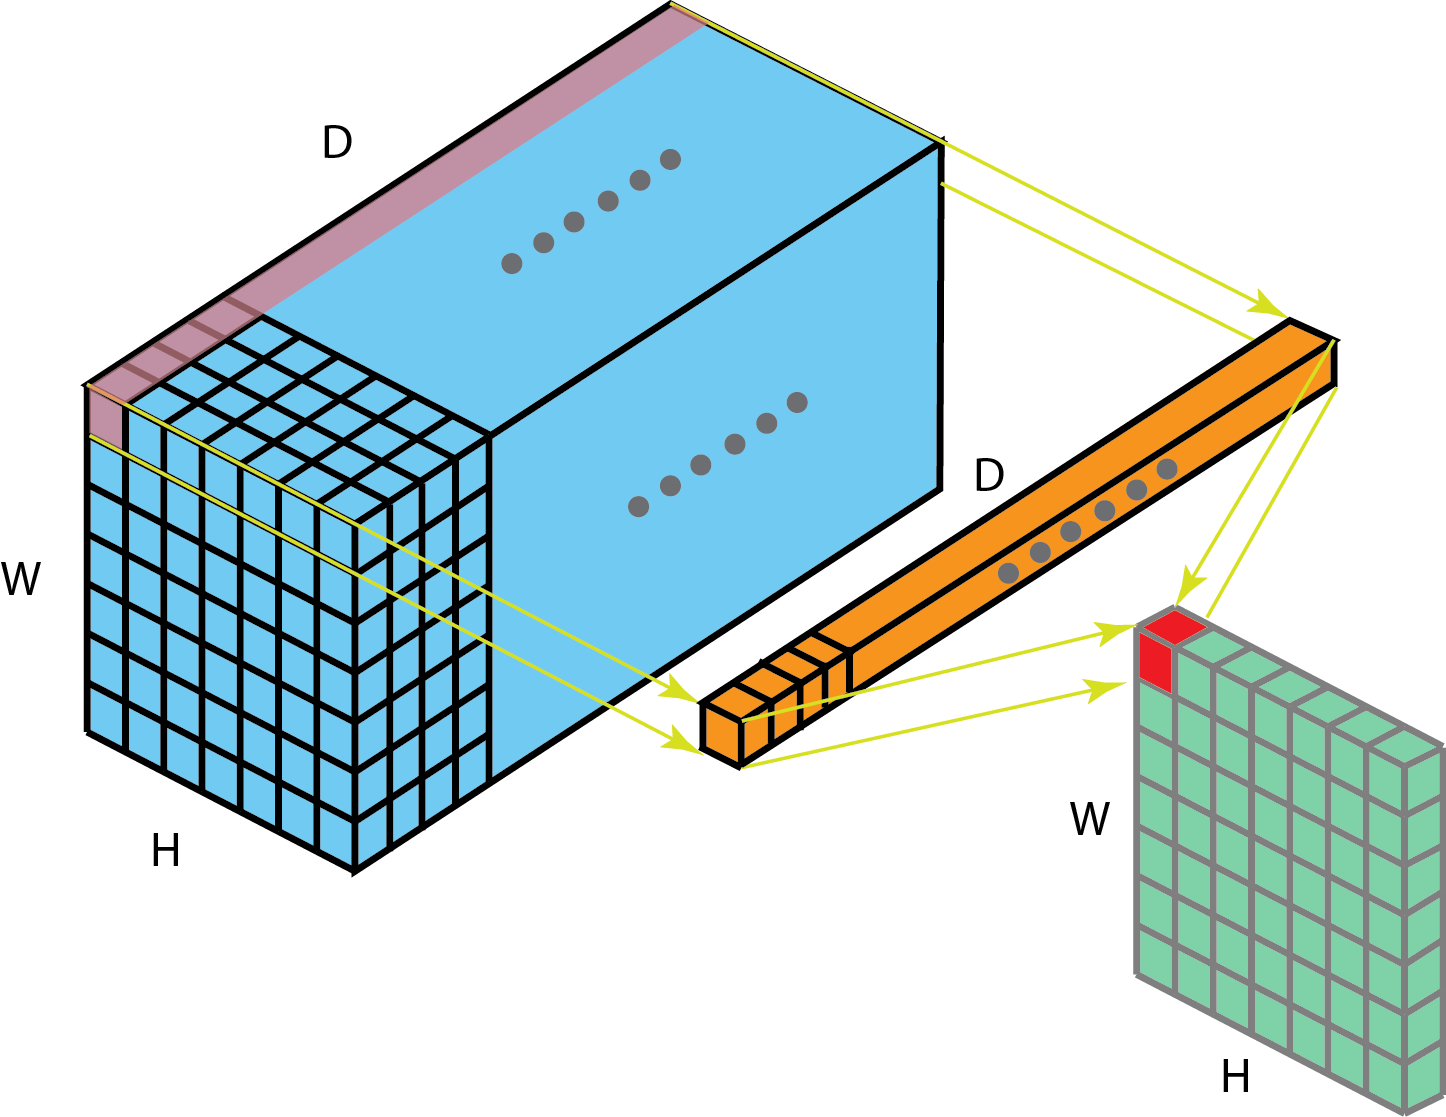
\includegraphics[width=.9\linewidth]{11conv.png}
%	\end{column}%
%\end{columns}
%\end{frame}
%
%
%
%
%\begin{frame}{GoogleLeNet aka Inception V1}
%\begin{center}
%	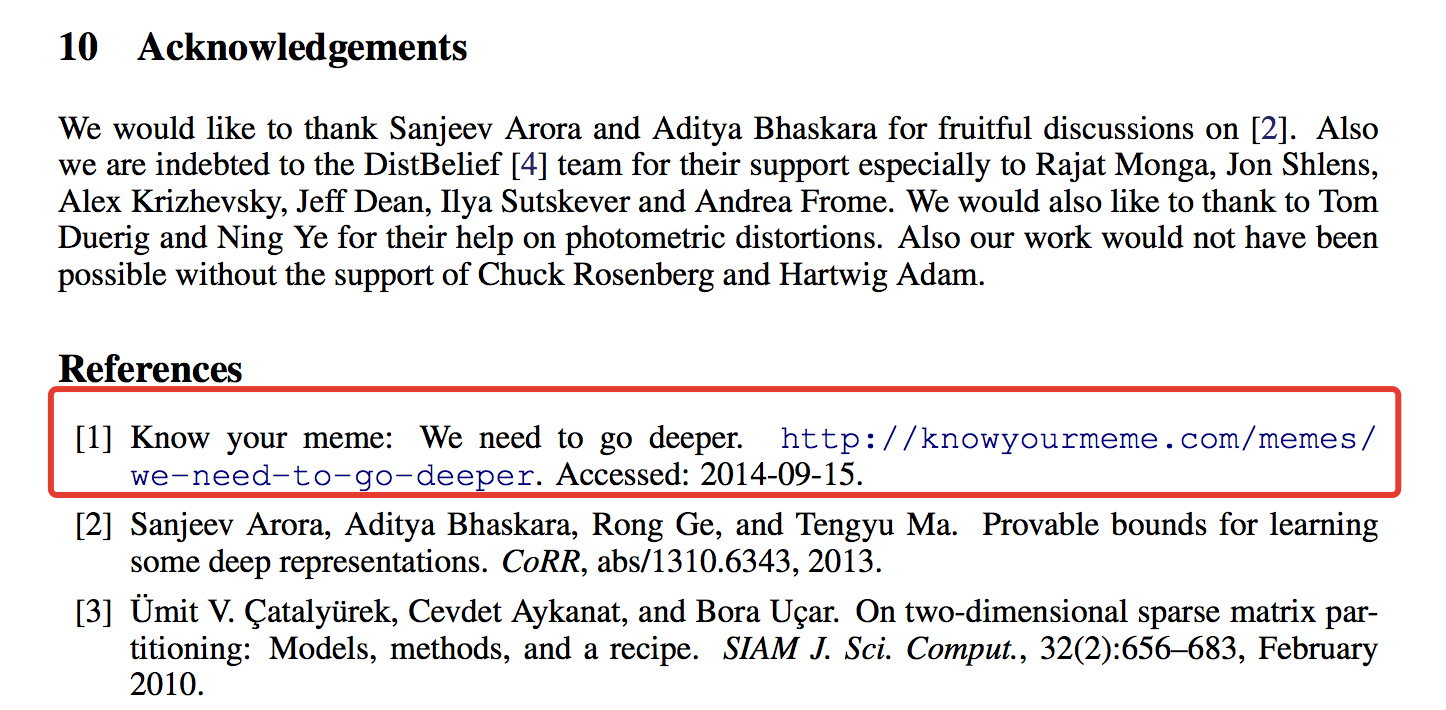
\includegraphics[width=.8\linewidth]{memes_incep.png}
%\end{center}
%\end{frame}
%
%
%\begin{frame}{Inception V3 (2015)}
%\begin{center}
%	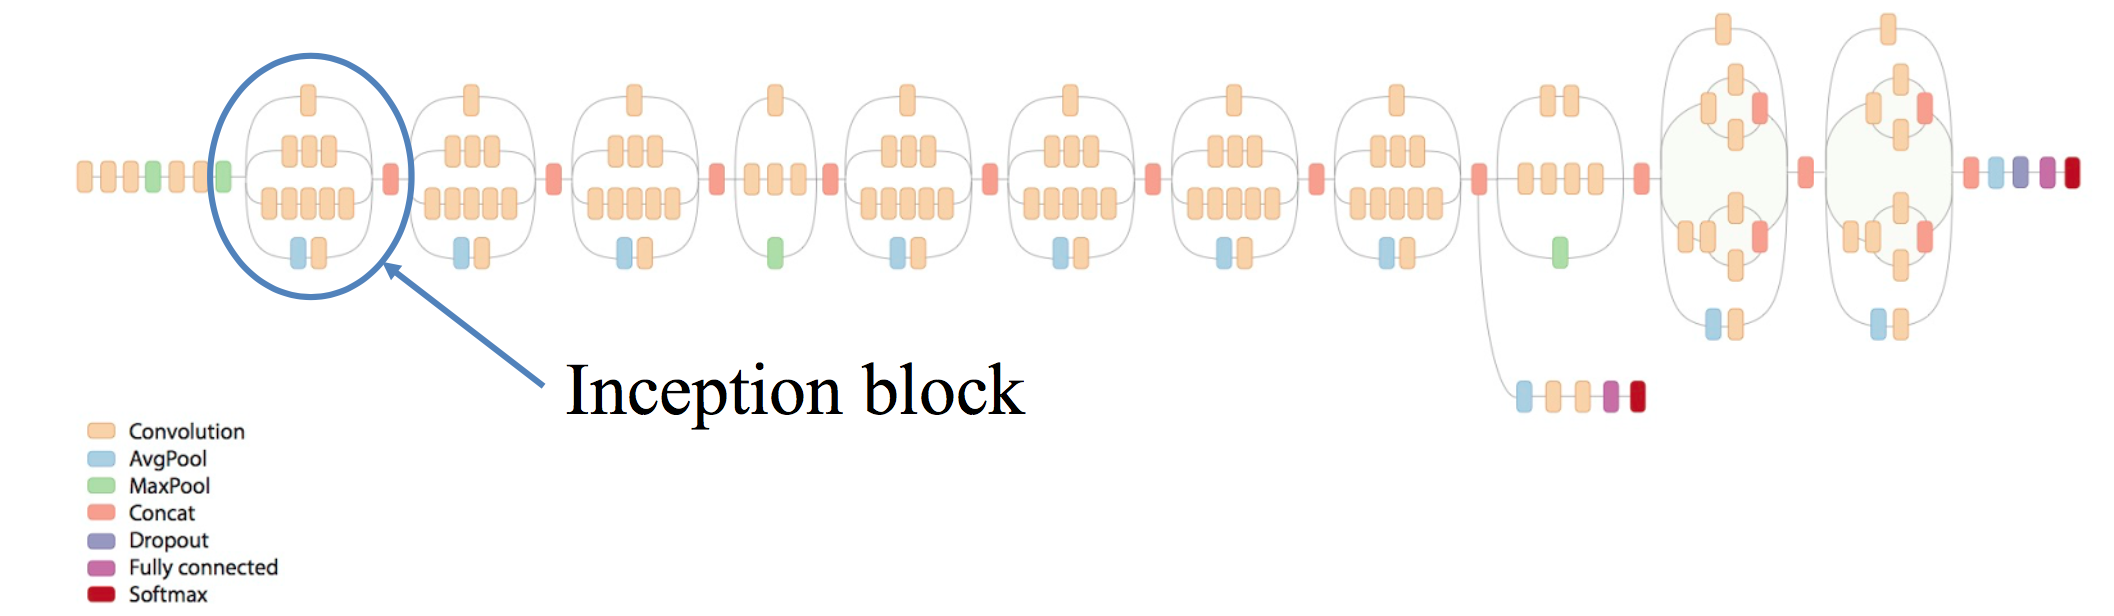
\includegraphics[width=.95\linewidth]{inception3.png}
%\end{center}
%\vfill %
%\footnotesize
%\color{blue} \url{https://arxiv.org/abs/1512.00567}
%\end{frame}
%
%
%\begin{frame}{Свёртка $n \times 1$ и $1 \times n$ }
%\begin{columns}[T] %
%	\begin{column}{.6\textwidth}
%	\centering	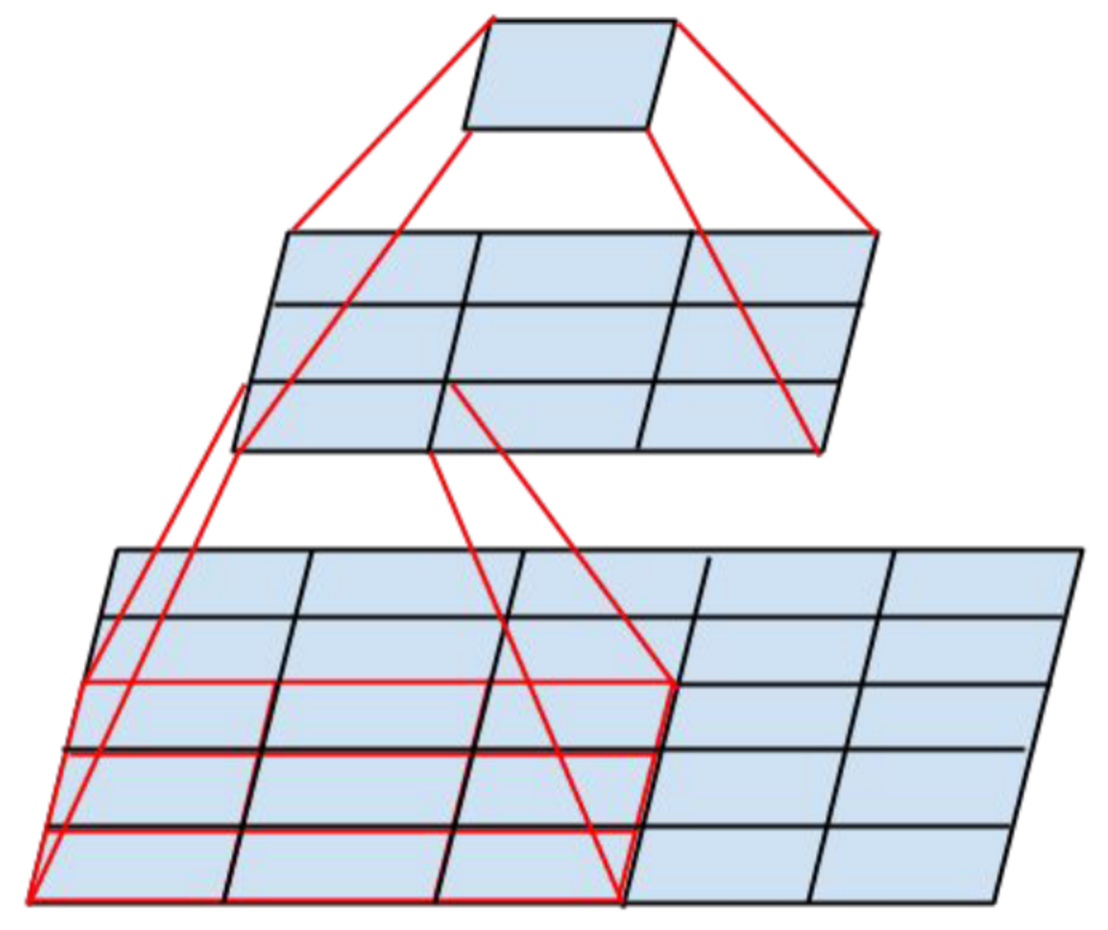
\includegraphics[width=.42\linewidth]{vgg_conv.png}
%	\end{column}%
%	\hfill%
%	\begin{column}{.4\textwidth}
%	\centering 	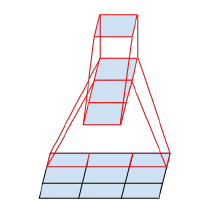
\includegraphics[width=.5\linewidth]{conv_inc_1.png} 
%	\end{column}%
%\end{columns}
%\vfill
%\begin{itemize}
%	\item В VGG заменяли большие свёртки на последовательные $3 \times 3$ для экономи
%	\item Пойдём дальше и заменим их на последовательные $3 \times 1$ и $1 \times 3$
%	\item Экономим ещё больше параметров, для каждой свёртки $6$ вместо $9$ 
%\end{itemize}
%\end{frame}
%
%\begin{frame}{Inception V3 (2015)}
%\begin{center}
%	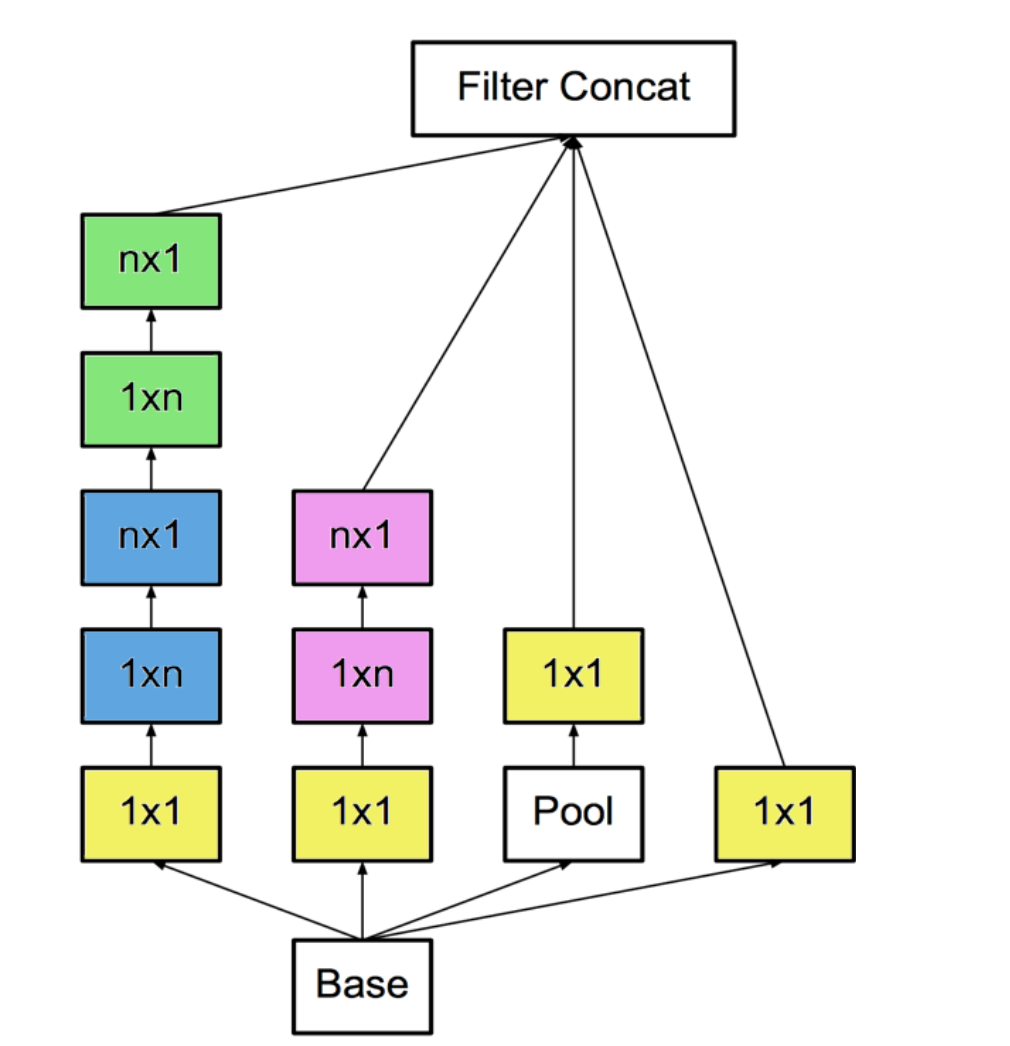
\includegraphics[width=.5\linewidth]{block3.png}
%\end{center}
%\end{frame}
%
%
%\begin{frame}{Inception V3 (2015)}
%\begin{wideitemize}
%	\item  Сетка собирается из $11$ inception layers, добавили BatchNorm (то же самое без него Inception V2)
%	
%	\item В результате исследований сформулировали принципы обучения глубоких свёрточных сетей: 
%	
%	\begin{enumerate}
%		\item  Избегайте representation bottlenecks, нельзя резко снижать размерность слоя, это надо делать плавно: от начала к концу
%		\item Свёртку нужно разбивать на более мелкие части для экономии ресурсов и увеличения размера сетки 
%		\item Нельзя резко увеличивать глубину, забивая на ширину, надо растить сбалансированно
%	\end{enumerate} 
%
%	\item Итоговое качество $4.2\%$ ошибок, ансамбль из $4$-х моделей дал $3.8\%$. 
%\end{wideitemize}
%\end{frame}
%
%
%\begin{frame}{ResNet (Microsoft) (2015)}
%\begin{center}
%	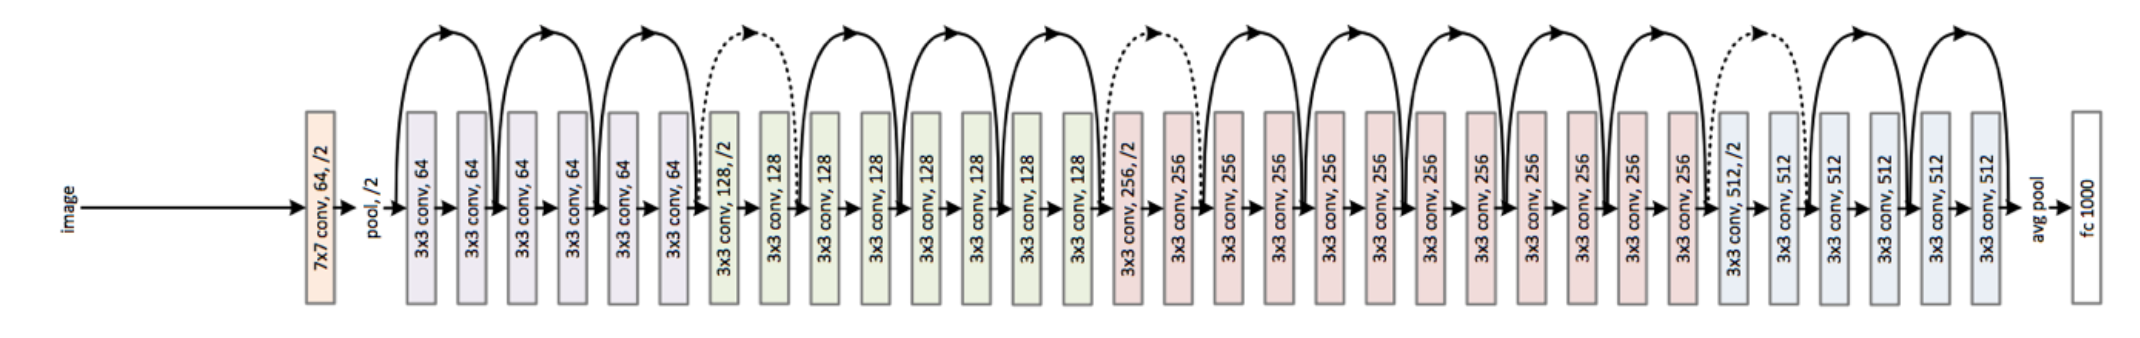
\includegraphics[scale=0.2]{resnet.png}
%\end{center}
%\begin{itemize}
%	\item 152 слоя, ошибка составила $3.75\%$, ансабль из сеток дал $3.57\%$
%\end{itemize}
%\vfill %
%\footnotesize
%\color{blue} \url{https://arxiv.org/abs/1512.03385}
%\end{frame}
%
%
%\begin{frame}{Завязочка}
%\begin{center}
%	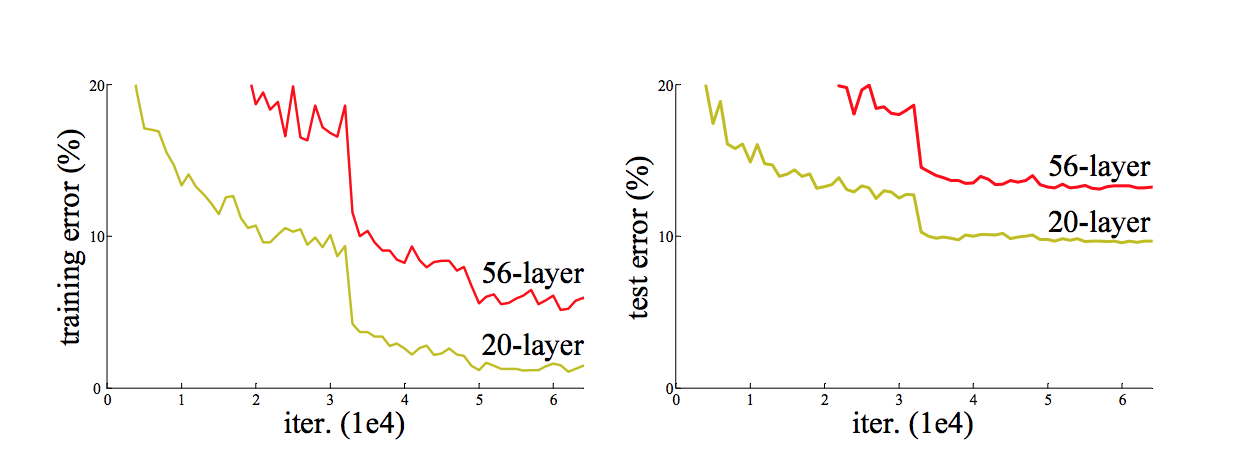
\includegraphics[scale=0.3]{resnet_idea.png}
%\end{center}
%\end{frame}
%
%
%\begin{frame}{Завязочка}
%\begin{wideitemize}
%	\item  VGG из $20$ слоёв и VGG из $56$ слоёв,  большая сетка обучается хуже
%	\item  \alert{Проблема:} слои инициализированы шумом, если какой-то один слой не натренирован, он убивает работу сети, через него не проходит полезный сигнал 
%	\item Чем больше слоёв, тем более ярко выражен этот эффект 
%	\item \alert{Решение:} Будем посылать вход на выход и давать слою возможность немного его подправить (residual слой)
%	\item Идея чем-то похожа на бустинг, сеть сама решает когда заканчивать подправлять выходы (грубо говоря, сама выбирает глубину)
%\end{wideitemize}
%\end{frame}
%
%
%\begin{frame}{ResNet (Microsoft) (2015)}
%\begin{center}
%	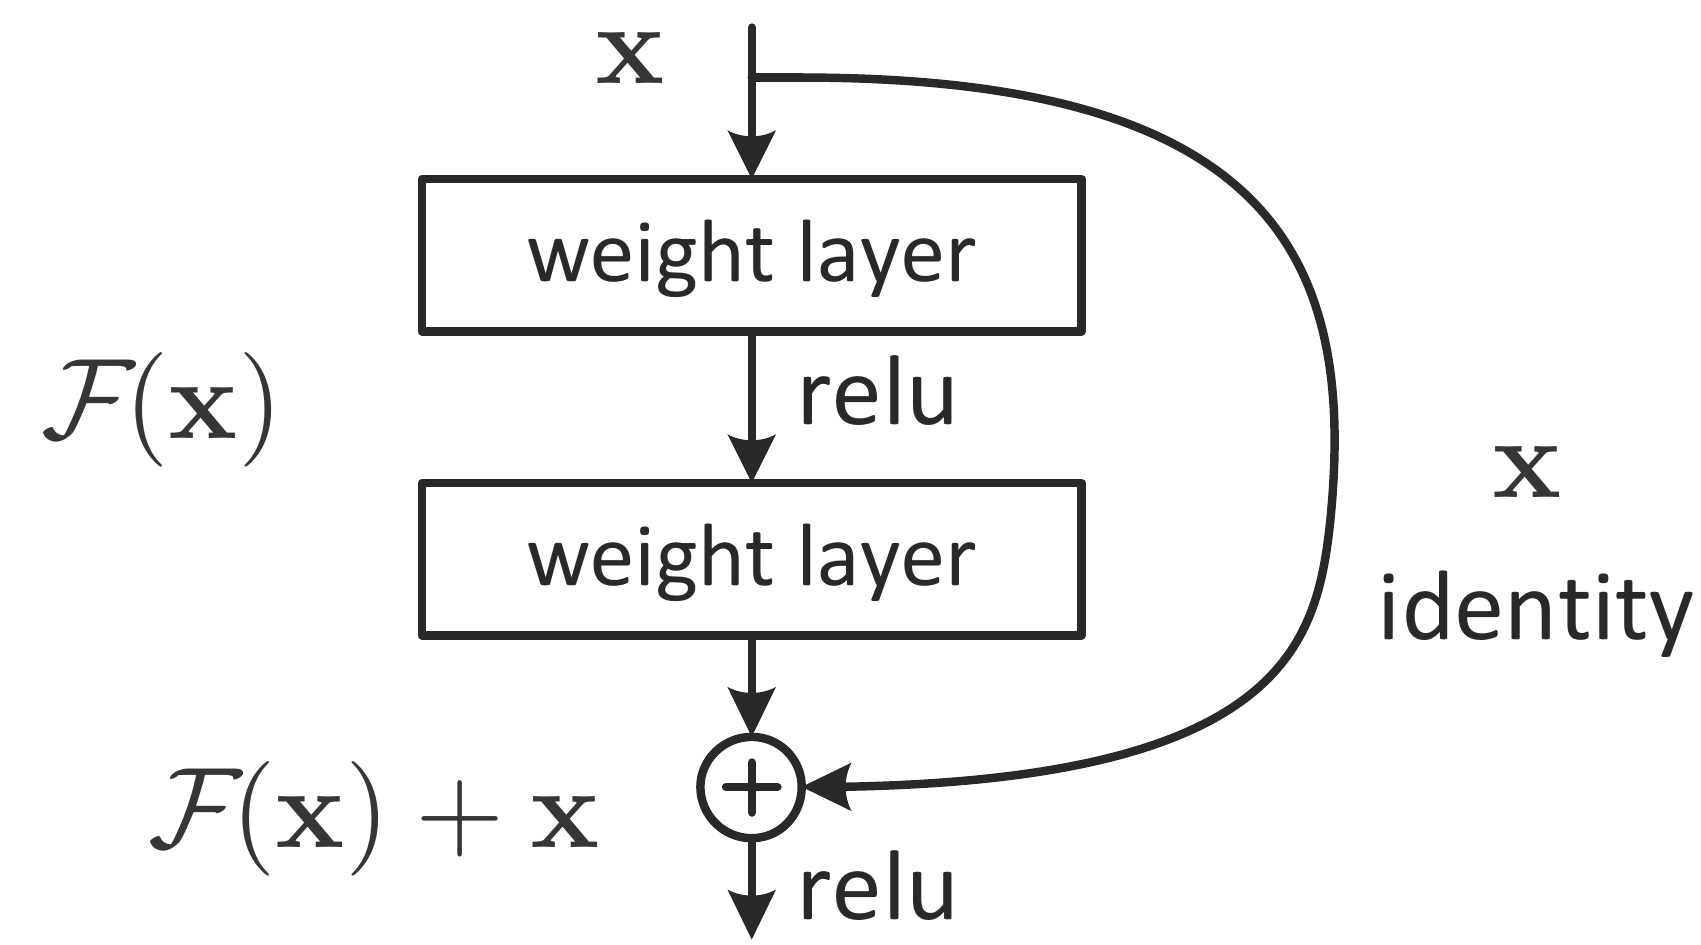
\includegraphics[scale=0.2]{resnet_layer.png}
%\end{center}
%\vfill %
%\footnotesize
%\color{blue} \url{https://arxiv.org/abs/1512.03385}
%\end{frame}
%
%
%
%\begin{frame}{ResNet (Microsoft) (2015)}
%\begin{wideitemize}
%	\item \alert{Идея:} более глубокие уровни должны улавливать разницу между новым и тем, что было раньше 
%	
%	\item Ключевым элементом архитектуры является связь, которая пропускает несколько слоёв, передавая результат предыдущего слоя
%	
%	\item Такое изменение позволило полностью отказаться от таких техник регуляризации, как DropOut
%	
%	\item Градиенты не взрываются, свойства ResNet активно пытаются сейчас изучать
%\end{wideitemize}
%\end{frame}
%
%
%\begin{frame}{Что было дальше?}
%\begin{wideitemize}
%	\item  В  2016 году Google попробовал Inception-Resnet и поставил ансамблем новый рекорд, $3.08\%$ 
%	\vfill
%	{\color{blue} \url{https://arxiv.org/abs/1602.07261}}
%	
%	\vfill
%	\item После Google задумались о переносе своих огромных архитектур в мобильные телефоны и стали работать над их компактностью 
%	\vfill 
%	{\color{blue} \url{https://ai.googleblog.com/2018/04/mobilenetv2-next-generation-of-on.html}}
%	
%	\vfill 
%	\item  В целом область развивается очень динамично и всплывает куча идей, на хабре иногда есть рубрика "Читаем статьи за вас", там можно посмотреть сколько идей возникло только за осень 2017
%	\vfill
%	{\color{blue} \url{https://habr.com/ru/company/ods/blog/343822/}}	
%\end{wideitemize}
%\end{frame}
%
%
%
% \begin{transitionframe}
%	\begin{center}
%		\Huge  Слайд из первой презентации :) 
%	\end{center}
%\end{transitionframe}
%
%\begin{frame}{\# 2. Сложность сетей растёт}
%%\begin{columns}[T] % align columns
%%	\begin{column}{.58\textwidth}
%\begin{center}
%	\includegraphics[width=.67\linewidth]{trend22.png}
%\end{center}
%%	\end{column}%
%%	\hfill%
%%\begin{column}{.38\textwidth}
%%	\begin{wideitemize}
%%		\item размер кружка - число параметров
%%		\item по $y$ точность на imagenet
%%		\item по $x$ число операций
%%	\end{wideitemize}	
%%\end{column}%
%%\end{columns}
%\vfill %
%\footnotesize
%\color{blue} \url{https://towardsdatascience.com/neural-network-architectures-156e5bad51ba}
%\end{frame} 


\end{document}
